\part{12/1}

\section{Stammfunktion bilden, integrieren}
\begin{gather*}
  \int_a^b x^7 \cdot dx = \left[\frac{1}{8}x^8\right]_a^b \\\\
  \int \frac{1}{(x + 4)^3} \cdot dx = -\frac{1}{2} \cdot (x + 4)^{-2} + c \\\\
  \int \frac{5}{(3x - 2)^5} \cdot dx = -\frac{5}{4 \cdot 3} \cdot (3x - 2)^{-4} + c \\\\
  \int \frac{1}{5} \cdot e^{2x} \cdot dx = \frac{1}{5 \cdot 2} \cdot e^{2x} + c
\end{gather*}
\section{bestimmtes Integral, Integralfunktion, unbestimmtes Integral}
\begin{gather*}
  \int_a^b \frac{1}{x} \cdot dx = \left[ln(|x|)\right]_a^b \\\\
  \text{sofern } a, b > 0 \text{ oder } a, b < 0 \text{ kein Problem} \\
  \text{wenn eines größer und eines kleiner $0$ ist, dann muss man genauer untersuchen (Polstelle!)} \\\\
  a = -1 \qquad b = 2 \\
  \int_a^b \frac{1}{2x - 5} \cdot dx = \left[\frac{1}{2} \cdot ln(|2x - 5|)\right]_a^b
\end{gather*}
\begin{exercise}{171/3}
  \item [a]
  \begin{gather*}
    \int_0^2 (2 + x)^3 \cdot dx = \left[\frac{1}{4} \cdot (2 + x)^4\right]_0^2 = \frac{1}{4} \cdot ((2 + 2)^4 - (2 + 0)^4) = 60
  \end{gather*}
  \item [b]
  \begin{gather*}
    \int_2^3 (1 + \frac{1}{x^2}) \cdot dx = \left[x - \frac{1}{x}\right]_2^3 = (3 - \frac{1}{3}) - (2 - \frac{1}{2}) = \frac{7}{6}
  \end{gather*}
  \item [c]
  \begin{gather*}
    \int_0^2 \frac{1}{(x + 1)^2} \cdot dx = \left[-(x + 1)^{-1}\right]_0^2 = -(2 + 1)^{-1} + (0 + 1)^{-1} = \frac{2}{3}
  \end{gather*}
  \item [d]
  \begin{gather*}
    \int_0^9 \frac{2}{5} \cdot \sqrt{x} \cdot dx = [\frac{4}{15} \cdot x^{\frac{3}{2}}]_0^9 = \frac{4}{15} \cdot 9^{\frac{3}{2}} - \frac{4}{15} \cdot 0^{\frac{3}{2}} = 7.2
  \end{gather*}
  \item [e]
  \begin{gather*}
    \int_{-0.5}^0 e^{2x + 1} \cdot dx = \left[\frac{1}{2}e^{2x + 1}\right]_{-0.5}^0 = \frac{1}{2}e^{2 \cdot 0 + 1} - \frac{1}{2}e^{2 \cdot (-0.5) + 1} \approx 0.8591
  \end{gather*}
  \item [f]
  \begin{gather*}
    \int_0^\pi sin(3x - \pi) \cdot dx = \left[-\frac{1}{3} \cdot cos(3x - \pi)\right]_0^\pi = \\ -\frac{1}{3} \cdot cos(3\pi - \pi) + \frac{1}{3} \cdot cos(3 \cdot 0 - \pi) = -\frac{2}{3}
  \end{gather*}
  \item [g]
  \begin{gather*}
    \int_{-1}^1 \frac{1}{5} \cdot e^{\frac{1}{2}x} \cdot dx = \left[\frac{2}{5}e^{\frac{1}{2}x}\right]_{-1}^1 = \frac{2}{5}e^{\frac{1}{2} \cdot 1} - \frac{2}{5}e^{\frac{1}{2} \cdot (-1)} = \frac{2e - 2}{5 \cdot \sqrt{e}} \approx 0.4169
  \end{gather*}
  \item [h]
  \begin{gather*}
    \int_{-\pi}^\pi cos(3x) \cdot dx = \left[-3 \cdot sin(3x)\right]_{-\pi}^\pi = -3 \cdot sin(3\pi) + 3 \cdot sin(3 \cdot (-\pi)) = 0
  \end{gather*}
\end{exercise}
\begin{exercise}{171/4}
  \item [c]
  \begin{gather*}
    \int_3^4 \frac{1}{2(x + 1)} \cdot dx = \left[\frac{ln(x + 1)}{2}\right]_3^4 = \frac{ln(4 + 1)}{2} - \frac{ln(3 + 1)}{2} \approx 0.1116
  \end{gather*}
\end{exercise}
\subsection{Integralfunktion}
\begin{gather*}
  \qquad\qquad \int_a^b f(x) \cdot dx = \left[F(x)\right]_a^b = F(b) - F(a) = J \\
  J_a(x) = \int_a^x f(x) \cdot dx = \left[F(x)\right]_a^x = F(x) - F(a)
\end{gather*}
Integralfunktion zur unteren (linken) Grenze $a$. Sie gibt zu jedem später eingesetzten Wert $x$ ($= b$) den bestimmten Integralwert an.
\begin{gather*}
  \int f(x) \cdot dx = \left[F(x)\right]^x = F(x) + c
\end{gather*}
unbestimmtes Integral
\begin{exercise}{175/2}
  \begin{gather*}
    f(x) = \frac{1}{2}x \qquad J_a(x) = \int_a^x \frac{1}{2}t \cdot dt
  \end{gather*} \\
  \begin{tabular}{l|cccccc}
    $x$ & $-4$ & $-2$ & $0$ & $2$ & $4$ & $6$ \\
    $J_{-4}(x)$ & $0$ & $-3$ & $-4$ & $-3$ & $0$ & $5$
  \end{tabular} \\\\\\
  \begin{tabular}{l|cccccc}
    $x$ & $-4$ & $-2$ & $0$ & $2$ & $4$ & $6$ \\
    $J_0(x)$ & $4$ & $1$ & $0$ & $1$ & $4$ & $9$
  \end{tabular} \\\\\\
  \begin{tabular}{l|cccccc}
    $x$ & $-4$ & $-2$ & $0$ & $2$ & $4$ & $6$ \\
    $J_2(x)$ & $3$ & $0$ & $-1$ & $0$ & $3$ & $8$
  \end{tabular}
\end{exercise}
\section{Rechenregeln für Integrale}
\begin{gather*}
  \int_a^a f(x) \cdot dx = 0 \\
  \int_a^b c \cdot f(x) \cdot dx = c \cdot \int_a^b f(x) \cdot dx \\
  \int_a^b f(x) \cdot dx + \int_b^c f(x) \cdot dx = \int_a^c f(x) \cdot dx \\
  \int_a^b f(x) \cdot dx = -\int_b^a f(x) \cdot dx \\
  \int_a^b f(x) \cdot dx \pm \int_a^b g(x) \cdot dx = \int_a^b (f(x) \pm g(x)) \cdot dx \\
\end{gather*}
\begin{exercise}{172/15}
  \item [a]
    \begin{gather*}
      \int_{-1}^{3.3} 5x^2 \cdot dx - 10 \cdot \int_{-1}^{3.3} \frac{1}{2}x^2 \cdot dx = 0
    \end{gather*}
  \item [b]
    \begin{gather*}
      \int_0^1 (x - 2\sqrt{x^2 + 4}) \cdot dx + 2 \cdot \int_0^1 \sqrt{x^2 + 4} \cdot dx = \int_0^1 x \cdot dx = 0.5
    \end{gather*}
  \item [c]
    \begin{gather*}
      \int_3^{3.7} \frac{1}{x} \cdot dx + \int_{3.7}^{4} \frac{1}{x} \cdot dx = \int_3^4 \frac{1}{x} \cdot dx = ln(4) - ln(3) \approx 0.2877
    \end{gather*}
\end{exercise}
\begin{exercise}{176/10}
  \begin{gather*}
    f(t) = 50t^4 \cdot e^{-t}
  \end{gather*}
  \item [a]
  Die Integralfunktion gibt die Anzahl der Telefonanrufe bis zum Zeitpunkt $x$ an.
  \begin{gather*}
    J_0(x) = \int_0^x f(t) \cdot dt \\
    J_0(4) = \int_0^4 f(t) \approx 445
  \end{gather*}
  \item [b]
  \begin{gather*}
    J_4(8) = J_0(8) - J_0(4) \approx 1080 - 445 = 635
  \end{gather*}
  Die Anzahl der Anrufer in der Warteschleife ist zu dem Zeitpunkt am höchsten, an dem die Anrufer pro Minute wieder unter $200$ sinken (bei $t \approx 5$).
\end{exercise}
\begin{exercise}{176/9}
  \begin{gather*}
    f(t) = cos(\frac{2\pi}{24}(t - 12)) \\
    g(t) = cos(\frac{2\pi}{24}(t - 6))
  \end{gather*}
  \item [a]
  Zunahme ($f(t) > 0$) zwischen $6$ und $18$ Uhr \\
  Abnahme ($f(t) < 0$) zwischen $18$ und $6$ Uhr \\\\
  Zunahme ($g(t) > 0$) zwischen $0$ und $12$ Uhr \\
  Abnahme ($g(t) < 0$) zwischen $12$ und $24$ Uhr
  \item [b]
  Am schnellsten um $12$ Uhr (Hochpunkt) \\
  Am langsamsten um $0$/$24$ Uhr (Tiefpunkt) \\\\
  Am schnellsten um $6$ Uhr (Hochpunkt) \\
  Am langsamsten um $18$ Uhr (Tiefpunkt)
  \item [c]
  Maximal um $18$ Uhr (Rechts-Links-Wendepunkt) \\
  Minimal um $6$ Uhr (Links-Rechts-Wendepunkt) \\\\
  Maximal um $12$ Uhr (Rechts-Links-Wendepunkt) \\
  Minimal um $0/24$ Uhr (Links-Rechts-Wendepunkt)
  \item [d]
  \begin{gather*}
    F(t) = -\frac{12}{\pi} \cdot sin(\frac{\pi}{12}t) + c \\
    c = 20 - F_{c=0}(12) = 20 \\
    F(18) \approx 23.82 \qquad F(6) \approx 16.18 \\\\
    G(t) = -\frac{12}{\pi} \cdot cos(\frac{\pi}{12}t) + c \\
    c = 20 - G_{c=0}(12) \approx 16.1803 \\
    G(12) = 20 \qquad G(0) = G(24) \approx 12.36
  \end{gather*}
\end{exercise}
\section{Ableitung der Umkehrfunktion}
\begin{gather*}
  \begin{tikzpicture}
    \begin{axis}[
      axis lines=middle,
      axis equal,
      xtick=\empty,
      ytick=\empty
      ]
      \addplot[
      domain=0:7,
      samples=20,
      dashed
      ]{x};
      \node[label={180:{$P$}},circle,fill,inner sep=2pt] at (axis cs:4,2) {};
      \node[label={270:{$\overline{P}$}},circle,fill,inner sep=2pt] at (axis cs:2,4) {};
      \draw[color=red] (axis cs:4,2) -- node[right]{$m=2$} (axis cs:4.5,3);
      \draw[color=red] (axis cs:2,4) -- node[above,xshift=16pt]{$m=\frac{1}{2}$} (axis cs:3,4.5);
      \draw[color=blue] (axis cs:4,2) -- node[below]{$m=-\frac{1}{3}$} (axis cs:5,1.67);
      \draw[color=blue] (axis cs:2,4) -- node[above,yshift=10pt]{$m=-3$} (axis cs:1.67,5);
    \end{axis}
  \end{tikzpicture}
\end{gather*}
\begin{gather*}
  f(x) = y = x^2 \Leftrightarrow \overline{f(y)} = x = \sqrt{y} \\
  \overline{f'(y)} = \frac{1}{f'(x)} \\\\
  \textbf{Beispiele} \\\\
  f(x) = y = x^2 \Leftrightarrow \overline{f(y)} = x = y^{\frac{1}{3}} \\
  \overline{f'(y)} = \frac{1}{3x^2} = \frac{1}{3(y^\frac{1}{3})^2} = \frac{1}{3}y^{-\frac{1}{3}} \\
  \text{umbenennen} \\
  \overline{f'(x)} = \frac{1}{3}x^{-\frac{1}{3}} \\\\
  f(x) = y = e^x \Leftrightarrow \overline{f(y)} = x = ln(y) \\
  \overline{f'(y)} = \frac{1}{e^x} = \frac{1}{e^{ln(x)}} = \frac{1}{y} \\
  \text{umbenennen} \\
  \overline{f'(x)} = \frac{1}{x}
\end{gather*}
\begin{gather*}
  f(x) = y = sin(x) \Leftrightarrow \overline{f(y)} = x = asin(y) \\
  \overline{f'(y)} = \frac{1}{cos(x)} = \frac{1}{cos(asin(y))} \\
  \;= \frac{1}{\sqrt{1 - sin^2(x)}} = \frac{1}{\sqrt{1 - sin^2(asin(y))}} = \frac{1}{\sqrt{1 - y^2}} \\
  \text{umbenennen} \\
  \overline{f'(x)} = \frac{1}{\sqrt{1 - x^2}}
\end{gather*}
\begin{gather*}
  f(x) = y = cos(x) \Leftrightarrow f(y) = x = acos(y) \\
  \overline{f'(y)} = \frac{1}{-sin(x)} = \frac{1}{-sin(acos(y))} \\
  \;= -\frac{1}{\sqrt{1 - cos^2(x)}} = -\frac{1}{\sqrt{1 - cos^2(acos(y))}} = -\frac{1}{\sqrt{1 - y^2}} \\
  \text{umbenennen} \\
  \overline{f'(x)} = -\frac{1}{\sqrt{1 - x^2}} \\\\
  f(x) = y = tan(x) \Leftrightarrow f(y) = x = atan(y) \\
  \overline{f'(y)} = cos^2(x) = cos^2(atan(y)) \\
  \;= 1 - sin^2(x) = 1 - sin^2(atan(y)) = 1 - \frac{y^2}{y^2 + 1} = \frac{1}{y^2 + 1} \\
  \text{umbenennen} \\
  \overline{f'(x)} = \frac{1}{x^2 + 1}
\end{gather*}
\section{Integral und Flächeninhalt}
\begin{figure}[H]
  \centering
  \includegraphics[width=0.8\textwidth]{/fakepath/integral_flaecheninhalt_1.png}
\end{figure}
\begin{gather*}
  A = A_1 + A_2 \\
  A \neq \int_a^b f(x) \cdot dx = I \\
  A = |\int_a^c f(x) \cdot dx| + |\int_c^b f(x) \cdot dx|
\end{gather*}
\begin{figure}[H]
  \centering
  \includegraphics[width=0.8\textwidth]{/fakepath/integral_flaecheninhalt_2.png}
\end{figure}
\begin{gather*}
  A = A_1 + A_2 \\
  \text{1. Berechne die Schnittstellen $a$, $b$, $c$} \\
  \text{2. } A = |\int_a^b (g(x) - f(x)) \cdot dx| + |\int_b^c (g(x) - f(x)) \cdot dx|
\end{gather*}
Wie die Flächen zur $x$-Achse liegen ist unwichtig, weil ich gedanklich beide Graphen gemeinsam soweit nach oben schieben kann dass die Flächen komplett oberhalb der $x$-Achse liegen.
\begin{gather*}
  f(x) \quad\longrightarrow\quad f(x) + d \\
  g(x) \quad\longrightarrow\quad g(x) + d
\end{gather*}
Durch Differenzialbildung fallen die gedanklich eingeführten Verschiebungen wieder weg.
\begin{gather*}
  \int_a^b ((f(x) + d) - (g(x) + d)) \cdot dx = \int_a^b (f(x) - g(x)) \cdot dx
\end{gather*}
\begin{exercise}{179/2}
  \item [a]
  \begin{gather*}
    f(x) = -0.5x^2 + 0.5 \qquad g(x) = -1.5 \\
    F(x) = -\frac{1}{6}x^3 + 0.5x \qquad G(x) = -1.5x
  \end{gather*}
  \begin{enumerate}[I]
    \item $A_2 + A_3$
    \begin{gather*}
      A = |\int_{-1}^1 f(x) \cdot dx| \\
      \;= |F(1) - F(-1)| = \frac{2}{3}FE
    \end{gather*}
    \item $A_2 + A_3 + A_4 + A_5$
    \begin{gather*}
      A = |\int_{-2}^2 (f(x) - g(x)) \cdot dx| \\
      \;= |(F(2) - F(-2)) - (G(2) - G(-2))| = 5\frac{1}{3}FE
    \end{gather*}
    \item $A_3$
    \begin{gather*}
      A = |\int_0^1 f(x) \cdot dx| \\
      \;= |F(1) - F(0)| = \frac{1}{3}FE
    \end{gather*}
    \item $A_1$
    \begin{gather*}
      A = |\int_{-2}^{-1} f(x) \cdot dx| \\
      \;= |F(-1) - F(-2)| = \frac{2}{3}FE
    \end{gather*}
  \end{enumerate}
\end{exercise}
\begin{exercise}{180/5}
  \item [a]
  \begin{gather*}
    f(x) = x^2 \qquad g(x) = -x^2 + 4x \\
    f(x) = g(x) \qquad L = \{0; 2\} \\
    f(x) - g(x) = 2x^2 - 4x \\
    A = |\int_0^2 (2x^2 - 4x) \cdot dx| = |[\frac{2}{3}x^3 - 2x^2]_0^2| = 2\frac{2}{3}FE
  \end{gather*}
  \item [b]
  \begin{gather*}
    f(x) = -\frac{1}{x^2} \qquad g(x) = 2.5x - 5.25 \\
    f(x) = g(x) \qquad L = \{2; \sim -0.4; \sim 0.5\} \\
    f(x) - g(x) = -2.5x + 5.25 - \frac{1}{x^2} \\
    A \approx |\int_{0.5}^2 (-2.5x + 5.25 - \frac{1}{x^2}) \cdot dx| \\
    \;= |[-1.25x^2 + 5.25x + \frac{1}{x}]_{0.5}^2| \approx 1.7FE
  \end{gather*}
\end{exercise}
\subsection{Flächeninhalt, uneigentliche Integrale}
\begin{exercise}{180/8}
  \begin{gather*}
    f_t(x) = \frac{t}{x^2} \qquad \left[1; 2\right] \\
    F_t(x) = -\frac{t}{x} \\
    A(t) = \int_1^2 -\frac{t}{x} \cdot dx = \frac{t}{2} \\
    A(16) = 8
  \end{gather*}
\end{exercise}
\begin{exercise}{180/10}
  \begin{gather*}
    f_a(x) = a \cdot sin(x) \qquad g_a(x) = -\frac{1}{a} \cdot sin(x) \qquad x \in \left[0; \pi\right] \\
    f_a(x) - g_a(x) = sin(x) \cdot (a + \frac{1}{a}) \\
    A(a) = \int_0^\pi sin(x) \cdot (a + \frac{1}{a}) \cdot dx = (a + \frac{1}{a}) \cdot \left[-cos(x)\right]_0^\pi = (a + \frac{1}{a}) \cdot 2 \\\\
    A'(a) = -\frac{2}{a^2} + 2 \\
    A''(a) = \frac{4}{a^3} \\
    A'(a) = 0 \qquad L = \{\pm1\} \\
    A''(1) = 4 > 0 \quad\Rightarrow\quad TP \\
    \text{Minimaler Flächeninhalt} \colon A(1) = 4FE
  \end{gather*}
\end{exercise}
\begin{gather*}
  \text{Beispiel } f(x) = \frac{1}{x^2} \qquad \left[3; \infty\right[ \\
  A = \lim\limits_{z \to \infty} \int_3^z \frac{1}{x^2} \cdot dx = \lim\limits_{z \to \infty} \left[-x^{-1}\right]_3^z \\
  \;= \lim\limits_{z \to \infty} (-\frac{1}{z} + \frac{1}{3}) = \frac{1}{3}FE
\end{gather*}
\begin{exercise}{183/1}
  \item [Fig. 1]
  \begin{gather*}
    y = \frac{1}{(x + 1)^2} \qquad \left[1; z\right] \\
    A(z) = \int_1^z \frac{1}{(x + 1)^2} \cdot dx = \left[-\frac{1}{x + 1}\right]_1^z = -\frac{1}{z + 1} + \frac{1}{2} \\
    A = \lim\limits_{z \to \infty} A(z) = \frac{1}{2}
  \end{gather*}
  \item [Fig. 2]
  \begin{gather*}
    y = e^{-\frac{1}{2}x} \qquad \left[2; z\right] \\
    A(z) = \int_2^z e^{-\frac{1}{2}x} \cdot dx = \left[-2 \cdot e^{-\frac{1}{2}x}\right]_2^z = -2 \cdot e^{-\frac{1}{2}z} + \frac{2}{e} \\
    A = \lim\limits_{z \to \infty} A(z) = \frac{2}{e} \approx 0.736
  \end{gather*}
  \item [Fig. 3]
  \begin{gather*}
    y = \frac{2}{x^3} \qquad \left[z; 1\right] \\
    A(z) = \int_z^1 \frac{2}{x^3} \cdot dx = \left[-\frac{1}{x^2}\right] = -1 + \frac{1}{z^2} \\
    A = \lim\limits_{z \to 0} A(z) = \infty
  \end{gather*}
  \item [Fig. 4]
  \begin{gather*}
    y = \frac{4}{\sqrt{x}} \qquad \left[z; 4\right] \\
    A(z) = \int_z^4 \frac{4}{\sqrt{x}} \cdot dx = \left[8 \cdot \sqrt{x}\right] = 16 - 8 \cdot \sqrt{z} \\
    A = \lim\limits_{z \to 0} A(z) = 16
  \end{gather*}
\end{exercise}
\begin{exercise}{183/7}
 \begin{gather*}
   W = \int_{h_1}^{h_2} F(s) \cdot ds \\
   F(s) = \gamma \frac{m \cdot M}{s^2} \\
   c = \gamma \cdot m \cdot M \approx 3.982 \cdot 10^{17} \cdot \frac{m \cdot kg}{s^2} \\
   F(s) = c \cdot s^{-2} \\
   W = \int_{h_1}^{h_2} c \cdot s^{-2} \cdot ds = \left[-c \cdot s^{-1}\right]_{h_1}^{h_2}
 \end{gather*}
 \item [a]
 \begin{gather*}
   h_1 = 6.37 \cdot 10^6m \qquad h_2 = 4.22 \cdot 10^7m \\
   W = \left[-c \cdot s^{-1}\right]_{6.37 \cdot 10^6m}^{4.22 \cdot 10^7m} \approx 1.333 \cdot 10^{-7} \cdot c \approx 5.308 \cdot 10^{10}Nm
 \end{gather*}
 \item [b]
 \begin{gather*}
   h_1 = 6.37 \cdot 10^6m \qquad h_2 \rightarrow \infty \\
   W = \lim\limits_{h_2 \to \infty} \left[-c \cdot s^{-1}\right]_{6.37 \cdot 10^6m}^{h_2} \approx 1.570 \cdot 10^{-7} \cdot c \approx 6.252 \cdot 10^{10}Nm
 \end{gather*}
\end{exercise}
\newpage
\begin{exercise}{183/5}
  \begin{enumerate}[I]
    \item $f(x) = \frac{1}{x^3} \qquad F(x) = -\frac{1}{2 \cdot x^2}$
    \item $f(x) = \frac{1}{x^2} \qquad F(x) = -\frac{1}{x}$
    \item $f(x) = \frac{1}{\sqrt{x}} \qquad F(x) = 2 \cdot \sqrt{x}$
  \end{enumerate}
  \item [a]
  \begin{gather*}
    \lim\limits_{z \to \infty} \int_1^z f(x) \cdot dx = \left[F(x)\right]_1^z
  \end{gather*}
  \begin{enumerate}[I]
    \item $= \frac{1}{2}$
    \item $= 1$
    \item $= \infty$
  \end{enumerate}
  \item [b]
  \begin{gather*}
    \lim\limits_{z \to 1} \int_z^0 f(x) \cdot dx = \left[F(x)\right]_z^1
  \end{gather*}
  \begin{enumerate}[I]
    \item $= \infty$
    \item $= \infty$
    \item $= 2$
  \end{enumerate}
\end{exercise}
\begin{exercise}{180/11}
  \begin{gather*}
    f(x) = x^2 \\
    t(x) = m \cdot x + b \\
    f'(x) = 2x \quad\Rightarrow\quad m = f'(a) = 2a \\
    f(a) = a^2 \quad\Rightarrow\quad b = a^2 - 2a \cdot a = -a^2 \\
    \Rightarrow t(x) = 2a \cdot x - a^2 \\\\
    \int_0^a (f(x) - t(x)) \cdot dx = \int_0^a (x^2 - 2ax + a^2) \cdot dx = \left[\frac{1}{3}x^3 - ax^2 + a^2x\right]_0^a \\
    \;= \frac{1}{3}a^3
  \end{gather*}
\end{exercise}
\section{Integration von Produkten: partielle Integration}
Ableitungs-Produktregel: $(u \cdot v)' = u' \cdot v + u \cdot v'$
\begin{gather*}
  (u \cdot v)' = u' \cdot v + u \cdot v' \equ - u \cdot v' \\
  u' \cdot v = (u \cdot v)' - u \cdot v' \equ \int \\
  \int u' \cdot v = \int (u \cdot v)' - \int u \cdot v' \\
  \int u' \cdot v = u \cdot v - \int u \cdot v' \\\\
  \textbf{Beispiel} \\
  \int sin(x) \cdot x \cdot dx = -cos(x) \cdot x - \int -cos(x) \cdot 1 \cdot dx \\
  \;= -cos(x) \cdot x + sin(x) + c \\
  (-cos(x)) \cdot x + sin(x))' = sin(x) \cdot x
\end{gather*}
\begin{gather*}
  \int e^{2x} \cdot x^2 \cdot dx = \frac{1}{2}e^{2x} \cdot x^2 - \int \frac{1}{2}e^{2x} \cdot 2x \cdot dx \\
  \;= \frac{1}{2}e^{2x} \cdot x^2 - (\frac{1}{2}e^{2x} \cdot x - \int \frac{1}{2}e^{2x} \cdot 1 \cdot dx) \\
  \;= \frac{1}{2}e^{2x} \cdot x^2 - \frac{1}{2}e^{2x} \cdot x + \int \frac{1}{2}e^{2x} \cdot dx \\
  \;= \frac{1}{2}e^{2x} \cdot x^2 - \frac{1}{2}e^{2x} \cdot x + \frac{1}{4}e^{2x} \\
  \;= e^{2x} \cdot (\frac{1}{2}x^2 - \frac{1}{2}x + \frac{1}{4})
\end{gather*}
Spezialfälle
\begin{gather*}
  \int 1 \cdot ln(x) \cdot dx = x \cdot ln(x) - \int x \cdot \frac{1}{x} \cdot dx \\
  \;= x \cdot ln(x) - x \\
  \text{(Stammfunktion von $ln(x)$)}
\end{gather*}
\begin{gather*}
  \int sin(x) \cdot cos(x) \cdot dx = -cos(x) \cdot cos(x) - \int cos(x) \cdot (-sin(x)) \cdot dx \\
  \;= -cos^2(x) - \int sin(x) \cdot cos(x) \cdot dx \equ + \int sin(x) \cdot cos(x) \cdot dx \\
  2 \cdot \int sin(x) \cdot cos(x) \cdot dx = -cos^2(x) \equ \div 2 \\
  \int sin(x) \cdot cos(x) \cdot dx = -\frac{cos^2(x)}{2}
\end{gather*}
\begin{exercise}{188/1}
  \item [a]
  \begin{gather*}
    \int_{-1}^{1} e^x \cdot x \cdot dx = \left[e^x \cdot x\right]_{-1}^{1} - \int e^x \cdot 1 \cdot dx = \left[e^x \cdot x - e^x\right]_{-1}^{1} = \frac{2}{e}
  \end{gather*}
  \item [d]
  \begin{gather*}
    \int_{0}^{0.5} e^{2x + 2} \cdot 4x \cdot dx = \left[\frac{1}{2}e^{2x + 2} \cdot 4x\right]_{0}^{0.5} - \int \frac{1}{2}e^{2x + 2} \cdot 4 \cdot dx \\
    \;= \left[2e^{2x + 2} \cdot x - e^{2x + 2}\right]_{0}^{0.5} = e^2
  \end{gather*}
\end{exercise}
\begin{exercise}{188/2}
  \item [b]
  \begin{gather*}
    \int_0^\pi cos(x) \cdot x \cdot dx = \left[sin(x) \cdot x\right]_0^\pi - \int sin(x) \cdot 1 \cdot dx \\
    \;= \left[sin(x) \cdot x + cos(x)\right]_0^\pi = -2
  \end{gather*}
  \item [d]
  \begin{gather*}
    \int_0^{2\pi} sin(0.5x) \cdot 2x \cdot dx = \left[-2cos(0.5x) \cdot 2x\right]_0^{2\pi} - \int -2cos(0.5x) \cdot 2 \cdot dx \\
    \;= \left[-2cos(0.5x) \cdot 2x + 8sin(0.5x)\right]_0^{2\pi} = 8\pi
  \end{gather*}
\end{exercise}
\newpage
\begin{exercise}{188/8}
  \item [a]
  \begin{gather*}
    \int_0^\pi (sin(x))^2 \cdot dx = \left[-cos(x) \cdot sin(x)\right]_0^\pi - \int -cos(x) \cdot cos(x) \cdot dx \\
    \;= \left[-cos(x) \cdot sin(x)\right]_0^\pi - \int (-sin^2(x) - 1) \cdot dx \\
    \;= \left[-cos(x) \cdot sin(x) + x\right]_0^\pi - \int sin^2(x) \cdot dx \equ + \int_0^\pi sin^2(x) \cdot dx; \quad \div 2 \\
    \;= \left[\frac{-cos(x) \cdot sin(x) + x}{2}\right]_0^\pi = \frac{\pi}{2}
  \end{gather*}
  \item [c]
  \begin{gather*}
    \int_{-2}^2 e^x \cdot cos(x) \cdot dx = \left[sin(x) \cdot e^x\right]_{-2}^2 - \int sin(x) \cdot e^x \cdot dx \\
    \;= \left[sin(x) \cdot e^x\right]_{-2}^2 - (\left[-cos(x) \cdot e^x\right]_{-2}^2 - \int -cos(x) \cdot e^x \cdot dx) \\
    \;= \left[sin(x) \cdot e^x + cos(x) \cdot e^x\right]_{-2}^2 - \int cos(x) \cdot e^x \cdot dx \\
    \;= \left[\frac{(sin(x) + cos(x)) \cdot e^x}{2}\right]_{-2}^2 \approx 1.912
  \end{gather*}
  \item [d]
  \begin{gather*}
    \int_0^2 sin(\pi x) \cdot e^{2x} \cdot dx = \left[\frac{1}{2}e^{2x} \cdot sin(\pi x)\right]_0^2 - \int \frac{1}{2}e^{2x} \cdot \pi \cdot cos(\pi x) \cdot dx \\
    \;= \left[\frac{1}{2}e^{2x} \cdot sin(\pi x)\right]_0^2 - (\left[\frac{1}{4}e^{2x} \cdot \pi \cdot cos(\pi x)\right]_0^2 - \int -\frac{1}{4}e^{2x} \cdot \pi^2 \cdot sin(\pi x) \cdot dx) \\
    \;= \left[\frac{1}{2}e^{2x} \cdot sin(\pi x)\right]_0^2 - (\left[\frac{1}{4}e^{2x} \cdot \pi \cdot cos(\pi x) + \frac{1}{4}\pi^2\right]_0^2 - \int e^{2x} \cdot sin(\pi x) \cdot dx) \\
    \;= \left[\frac{2e^{2x} \cdot sin(\pi x) - \pi \cdot e^{2x} \cdot cos(\pi x)}{\pi^2 + 4}\right]_0^2 = \frac{\pi}{\pi^2 + 4} - \frac{e^4 \cdot \pi}{\pi^2 + 4} \approx -12.140
  \end{gather*}
\end{exercise}
\section{Integration durch Substitution}
Kettenregel: $(f(g(x)))' = f'(g(x)) \cdot g'(x)$ \\
\begin{gather*}
  \int f'(g(x)) \cdot g'(x) \cdot dx = \int (f(g(x)))' \cdot dx \\
  \;= f(g(x)) \qquad \text{Dabei ist $f$ die Stammfunktion von $f'$} \\
  \Rightarrow \text{ Benenne um $f' \rightarrow f \qquad f \rightarrow F$} \\\\
  \int f(g(x)) \cdot g'(x) \cdot dx = F(g(x)) \\\\
  \text{Substitution 1} \\
  \int_a^b f(g(x)) \cdot g'(x) \cdot dx \qquad \text{ersetze $z = g(x) \qquad \frac{dz}{dx} = g'(x) \Rightarrow dz = g'(x) \cdot dx$} \\
  \;= \int_{g(a)}^{g(b)} f(z) \cdot dz = \left[F(z)\right]_{g(a)}^{g(b)} \\
  \text{Resubstitution} \\
  \;= \left[F(g(x))\right]_a^b
\end{gather*}
Beispiel
\begin{gather*}
  \int_1^2 \frac{5x}{\sqrt{1 + 3x^2}} \cdot dx \\\\
  \text{subst. } z = 1 + 3x^2 \qquad \frac{dz}{dx} = (1 + 3x^2)' = 6x \qquad dz = 6x \cdot dx \\
  \;= {\color{red}\frac{5}{6}} \int_1^2 \frac{{\color{red}6}x}{\sqrt{1 + 3x^2}} \cdot dx = \frac{5}{6} \int_4^{13} z^{-\frac{1}{2}} \cdot dz \\
  \;= \frac{5}{6} \left[2z^\frac{1}{2}\right]_4^{13} = \frac{5}{6} \left[2 \cdot (1 + 3x^2)^\frac{1}{2}\right]_1^2 \approx 2.676
\end{gather*}
\newpage
\begin{exercise}{191/1}
  \item [a]
  \begin{gather*}
    \int_0^2 \frac{4x}{\sqrt{1 + 2x^2}} \cdot dx; \qquad g(x) = 1 + 2x^2 \\
    \text{subst. } z = g(x) \qquad dz = g'(x) \cdot dx \\
    \;= \int_{g(0)}^{g(2)} \frac{1}{\sqrt{z}} \cdot dz = \left[2 \cdot \sqrt{z}\right]_1^9 = 4
  \end{gather*}
  \item [b]
  \begin{gather*}
    \int_{-1}^1 \frac{-2x}{(4 - 3x^2)^2} \cdot dx; \qquad g(x) = 4 - 3x^2 \\
    \text{subst. } z = g(x) \qquad dz = g'(x) \cdot dx \\
    \;= \int_{g(-1)}^{g(1)} \frac{1}{3z^2} \cdot dz = \left[-\frac{1}{3z}\right]_1^1 = 0
  \end{gather*}
\end{exercise}
\begin{exercise}{191/3}
  \item [e]
  \begin{gather*}
    \int_0^3 \frac{2x}{1 + x^2} \cdot dx \\
    \text{subst. } z = 1 + x^2 \qquad dz = 2x \cdot dx \\
    \;= \int_1^{10} \frac{1}{z} \cdot dz = \left[ln(z)\right]_1^{10} \\
    \text{resubst.} \\
    \;= \left[ln(1 + x^2)\right]_0^3 = ln(10) \approx 2.3026
  \end{gather*}
  \item [f]
  \begin{gather*}
    \int_{-1}^2 \frac{e^x}{2 + e^x} \cdot dx \\
    \text{subst. } z = 2 + e^x \qquad dz = e^x \cdot dx \\
    \;= \int_{2 + e^{-1}}^{2 + e^2} \frac{1}{z} \cdot dz = \left[ln(z)\right]_{2 + e^{-1}}^{2 + e^2} \\
    \text{resubst.} \\
    \;= \left[ln(2 + e^x)\right]_{-1}^2 \approx 1.3775
  \end{gather*}
  \item [g]
  \begin{gather*}
    \int_e^{e^2} \frac{4}{x \cdot ln(x)} \cdot dx \\
    \text{subst. } z = ln(x) \qquad dz = \frac{1}{x} \cdot dx \\
    \;= \int_1^2 \frac{4}{z} \cdot dz = \left[4 \cdot ln(z)\right]_1^2 \\
    \text{resubst.} \\
    \;= \left[4 \cdot ln(ln(x))\right]_e^{e^2} = 4 \cdot ln(2) \approx 2.7726
  \end{gather*}
  \item [h]
  \begin{gather*}
    \int_\frac{1}{3}^\frac{1}{2} \frac{\pi \cdot cos(\pi x)}{sin(\pi x)} \cdot dx \\
    \text{subst. } z = sin(\pi x) \qquad dz = \pi \cdot cos(\pi x) \cdot dx \\
    \;= \int_{sin(\frac{\pi}{3})}^{sin(\frac{\pi}{2})} \frac{1}{z} \cdot dz = \left[ln(z)\right]_{sin(\frac{\pi}{3})}^{sin(\frac{\pi}{2})} \\
    \text{resubst.} \\
    \;= \left[ln(sin(\pi x))\right]_\frac{1}{3}^\frac{1}{2} \approx 0.1438
  \end{gather*}
\end{exercise}
\begin{exercise}{191/8}
  \item [a]
  \begin{gather*}
    \int_0^{ln(2)} \frac{e^{2x}}{e^{2x} + 3} \cdot dx \qquad\qquad t = e^{2x} + 3 \qquad t' = \frac{dt}{dx} = 2e^{2x} \qquad dx = \frac{1}{2 \cdot e^{2x}} \cdot dt \\
    \;= \int_{t(0)}^{t(ln(2))} \frac{e^{4x}}{t} \cdot \frac{1}{2 \cdot e^{2x}} \cdot dt = \int_{t(0)}^{t(ln(2))} \frac{e^{2x}}{2t} \cdot dt = \int_{t(0)}^{t(ln(2))} \frac{t - 3}{2t} \cdot dt \\
    \;= \left[\frac{t}{2} - \frac{3}{2} \cdot ln(t)\right]_4^7 \approx 0.6606
  \end{gather*}
  \item [b]
  \begin{gather*}
    \int_1^2 \frac{2x + 3}{(x + 2)^2} \cdot dx \qquad\qquad t = x + 2 \qquad t' = \frac{dt}{dx} = 1 \qquad dx = dt \\
    \;= \int_{t(1)}^{t(2)} \frac{2x + 3}{t^2} \cdot dt = \int_{t(1)}^{t(2)} \frac{2t - 1}{t^2} \cdot dt = \int_{t(1)}^{t(2)} (\frac{2}{t} - \frac{1}{t^2}) \cdot dt \\
    \;= \left[2 \cdot ln(t) + \frac{1}{t}\right]_3^4 \approx 0.4920
  \end{gather*}
  \item [c]
  \begin{gather*}
    \int_{0.5}^7 \frac{x}{\sqrt{4x - 1}} \cdot dx \qquad\qquad t = 4x - 1 \qquad t' = \frac{dt}{dx} = 4 \qquad dx = \frac{dt}{4} \\
    \;= \int_{t(0.5)}^{t(7)} \frac{x}{\sqrt{t}} \cdot \frac{1}{4} \cdot dt = \int_{t(0.5)}^{t(7)} \frac{\frac{1}{4}t + \frac{1}{4}}{4 \cdot \sqrt{t}} \cdot dt = \int_{t(0.5)}^{t(7)} \frac{t + 1}{16 \cdot \sqrt{t}} \cdot dt \\
    \;= \left[(\frac{1}{16}t + \frac{1}{16}) \cdot 2 \cdot \sqrt{t}\right]_{t(0.5)}^{t(7)} - \int_{t(0.5)}^{t(7)} \frac{1}{8} \cdot \sqrt{t} \cdot dt \\
    \;= \left[(\frac{1}{8}t + \frac{1}{8}) \cdot \sqrt{t}\right]_{t(0.5)}^{t(7)} - \left[\frac{1}{8} \cdot \frac{2}{3} \cdot \sqrt{t^3}\right]_{t(0.5)}^{t(7)} \\
    \;= \left[\frac{1}{8} \cdot (t \cdot \sqrt{t} + \sqrt{t} - \frac{2}{3} \cdot \sqrt{t^3})\right]_1^{27} \approx 6.3285
  \end{gather*}
  \item [d]
  \begin{gather*}
    \int_0^4 \frac{4}{1 + 2 \cdot \sqrt{x}} \cdot dx \qquad\qquad t = 1 + 2 \cdot \sqrt{x} \qquad t' = \frac{dt}{dx} = \frac{1}{\sqrt{x}} \qquad dx = \sqrt{x} \cdot dt \\
    \;= \int_{t(0)}^{t(4)} \frac{4}{t} \cdot \sqrt{x} \cdot dt = \int_{t(0)}^{t(4)} \frac{4}{t} \cdot \frac{t - 1}{2} \cdot dt = \int_{t(0)}^{t(4)} \frac{4t - 4}{2t} \cdot dt \\
    \;= \left[\frac{1}{2t} \cdot (2t^2 - 4t)\right]_{t(0)}^{t(4)} - \int_{t(0)}^{t(4)} - \frac{1}{2t^2} \cdot (2t^2 - 4t) \cdot dt \\
    \;= \left[t - 2\right]_{t(0)}^{t(4)} - \int_{t(0)}^{t(4)} (\frac{2}{t} - 1) \cdot dt \\
    \;= \left[t - 2 - (2 \cdot ln(t) - t)\right]_{t(0)}^{t(4)} = \left[2 \cdot (t - 1 - ln(t))\right]_1^5 \approx 4.7811
  \end{gather*}
\end{exercise}
\begin{gather*}
  \text{Substitution 2} \\
  \int_a^b f(x) \cdot dx \qquad \text{ersetze } x = g(z) \\
  \;= \int_a^b f(g(z)) \cdot dx = \int_{\overline{g}(a)}^{\overline{g}(b)} f(g(z)) \cdot g'(z) \cdot dz \\\\
  \qquad x = g(z) \qquad z = \overline{g}(x) \\
  \qquad \frac{dx}{dz} = g'(z) \qquad dx = g'(z) \cdot dz \\\\
  \;= \left[F(g(z))\right]_{\overline{g}(a)}^{\overline{g}(b)} = \left[F(x)\right]_a^b
\end{gather*}
Beispiel
\begin{gather*}
  \int_0^\frac{1}{2} \frac{1}{\sqrt{1 - x^2}} \cdot dx \qquad x = sin(z) \qquad dx = cos(z) \cdot dz \\
  \;= \int_0^\frac{\pi}{6} \frac{cos(z)}{\sqrt{1 - sin^2(z)}} \cdot dz = \int_0^\frac{\pi}{6} 1 \cdot dz = \left[z\right]_0^\frac{\pi}{6} = \frac{\pi}{6} \approx 0.524
\end{gather*}
\begin{exercise}{AB/23}
  \item [a]
  \begin{gather*}
    \int_0^1 e^x \cdot \sqrt{e^x + 1} \cdot dx \\
    x(t) = ln(t) \qquad t = e^x \qquad dx = \frac{1}{t} \cdot dt \\
    \;= \int_{e^0}^{e^1} e^{ln(t)} \cdot \sqrt{e^{ln(t)} + 1} \cdot \frac{1}{t} \cdot dz = \int_1^e \sqrt{t + 1} \cdot dz \\
    \;= \left[\frac{2}{3} \cdot \sqrt{(t + 1)^3}\right]_1^e \approx 2.8943
  \end{gather*}
  \item [c]
  \begin{gather*}
    \int_1^3 \frac{1}{x} \cdot ln(x^2) \cdot dx \\
    x(t) = e^t \qquad t = ln(x) \qquad dx = e^t \cdot dt \\
    \;= \int_{ln(1)}^{ln(3)} \frac{1}{e^t} \cdot ln(e^{t^2}) \cdot e^t \cdot dt = \int_0^{ln(3)} ln(e^{2t}) \cdot dt = \int_0^{ln(3)} 2t \cdot dt \\
    \;= \left[t^2\right]_0^{ln(3)} = (ln(3))^2 \approx 1.2069
  \end{gather*}
\end{exercise}
\subsection{Wiederholung}
\begin{enumerate}
  \item Ersetze $g(x)$ durch $z$
  \begin{gather*}
    \int_a^b = f(g(x)) \cdot g'(x) \cdot dx = \int_{g(a)}^{g(b)} f(z) \cdot dz \\
    \;= \left[F(z)\right]_{g(a)}^{g(b)} = \left[F(g(x))\right]_a^b \\
    z = g(x) \\\\
    \frac{dz}{dx} = g'(x) \\
    dz = g'(x) \cdot dx
  \end{gather*}
  \item Ersetze $x$ durch $g(z)$
  \begin{gather*}
    \int_a^b f(x) \cdot dx = \int_{\overline{g}(a)}^{\overline{g}(b)} f(g(z)) \cdot g'(z) \cdot dz \\
    \;= \left[F(g(z))\right]_{\overline{g}(a)}^{\overline{g}(b)} = \left[F(x)\right]_a^b \\\\
    x = g(z) \quad\Leftrightarrow\quad z = \overline{g}(x) \\
    \frac{dx}{dz} = g'(z) \\
    dx = g'(z) \cdot dz
  \end{gather*}
\end{enumerate}
\begin{exercise}{AB/23}
  \item [d]
  \begin{gather*}
    \int_1^2 \frac{1 + ln(x)}{x \cdot (1 - ln(x))} \cdot dx \\
    x(t) = e^t \qquad t = ln(x) \qquad dx = e^t \cdot dt \\\\
    \;= \int_{ln(1)}^{ln(2)} \frac{1 + ln(e^t)}{e^t \cdot (1 - ln(e^t))} \cdot e^t \cdot dt = \int_0^{ln(2)} \frac{1 + t}{1 - t} \cdot dt \\
    z = 1 - t \qquad \frac{dz}{dt} = -1 \qquad dz = -dt \\\\
    \;= -\int_{1 - 0}^{1 - ln(2)} \frac{2 - z}{z} \cdot dz = -\int_{1 - 0}^{1 - ln(2)} (\frac{2}{z} - 1) \cdot dz \\
    \;= -\left[2 \cdot ln(z) - z\right]_1^{1 - ln(2)} \approx 1.6696
  \end{gather*}
  \item [g]
  \begin{gather*}
    \int_0^1 \frac{1}{\sqrt{4 - x^2}} \cdot dx \\
    x(t) = 2 \cdot sin(t) \qquad t = asin(\frac{x}{2}) \qquad dx = 2 \cdot cos(t) \cdot dt \\\\
    \;= \int_{asin(\frac{0}{2})}^{asin(\frac{1}{2})} \frac{2 \cdot cos(t)}{\sqrt{4 - (2 \cdot sin(t))^2}} \cdot dt = \int_0^{asin(\frac{1}{2})} \frac{2 \cdot cos(t)}{2 \cdot \sqrt{1 - (sin(t))^2}} \cdot dt \\
    \;= \int_0^{asin(\frac{1}{2})} \frac{2 \cdot cos(t)}{2 \cdot \sqrt{(cos(t))^2}} \cdot dt = \int_0^{asin(\frac{1}{2})} 1 \cdot dt = \left[t\right]_0^{asin(\frac{1}{2})} = \frac{\pi}{6}
  \end{gather*}
\end{exercise}
\section{Rotationskörper}
Rotationssymetrische Körper, die man sich dadurch entstanden vorstellen kann, dass eine Fläche um eine Achse ($x$-Achse) rotiert.
\subsection{Bestimmung des Volumens von Rotationskörpern}
\begin{gather*}
  f(x) = \frac{1}{2}x^2 + 1
\end{gather*}
\begin{figure}[H]
  \centering
  \includegraphics[width=1.1\textwidth]{/fakepath/rotationskoerper.png}
\end{figure}
\begin{gather*}
  A = \int_a^b f(x) \cdot dx \\
  \;= \int_1^2 (\frac{1}{2}x^2 + 1) \cdot dx = \left[\frac{1}{6}x^3 + x\right]_1^2 = \frac{13}{6} FE \approx 2.17FE \\
  V = \int_a^b \pi \cdot (f(x))^2 \cdot dx \\
  \;= \pi \cdot \int_1^2 (\frac{1}{2}x^2 + 1)^2 \cdot dx = \pi \cdot \left[\frac{1}{20}x^5 + \frac{1}{3}x^3 + x\right]_1^2 = \frac{293\pi}{60}VE \approx 15.34VE
\end{gather*}
\newpage
\begin{exercise}{196/1}
  \item [a]
  \begin{gather*}
    y = \sqrt{x + 1} \\
    V = \pi \cdot \int_{-1}^2 (\sqrt{x + 1})^2 \cdot dx = \pi \cdot \int_{-1}^2 (x + 1) \cdot dx \\
    \;= \pi \cdot \left[\frac{1}{2}x^2 + x\right]_{-1}^2 = \pi \cdot 4.5VE \approx 14.1372VE
  \end{gather*}
  \item [b]
  \begin{gather*}
    y = \frac{1}{x} \\
    V = \pi \cdot \int_1^3 (\frac{1}{x})^2 \cdot dx = \pi \cdot \int_1^3 x^{-2} \cdot dx \\
    \;= \pi \cdot \left[-x^{-1}\right]_1^3 = \pi \cdot \frac{2}{3}VE \approx 2.0944VE
  \end{gather*}
  \item [c]
  \begin{gather*}
    y = x^2 - 6x + 8 \\
    y = 0 \qquad L = \{2; 4\} \\
    V = \pi \cdot \int_2^4 (x^2 - 6x + 8)^2 \cdot dx = \pi \cdot \int_2^4 (x^4 - 12x^3 + 52x^2 - 96x + 64) \cdot dx \\
    \;= \pi \cdot \left[\frac{1}{5}x^5 - 3x^4 + \frac{52}{3}x^3 - 48x^2 + 64x\right]_2^4 = \pi \cdot \frac{16}{15}VE \approx 3.3510VE
  \end{gather*}
\end{exercise}
\begin{exercise}{197/8}
  \begin{gather*}
    f(x) = 0.5x + 1 \qquad g(x) = 1.5 \cdot \sqrt{x - 1} \qquad \left[0; 4\right]
  \end{gather*}
  \item [a]
  \begin{gather*}
    V_W = \pi \cdot \int_1^4 (1.5 \cdot \sqrt{x - 1})^2 \cdot dx = \pi \cdot \int_1^4 (2.25x - 2.25) \cdot dx \\
    \;= \pi \cdot \left[1.125x^2 - 2.25x\right]_1^4 = 10.125\pi \approx 31.8086 \\
    [V_W] = cm^3
  \end{gather*}
  \item [b]
  \begin{gather*}
    V = \pi \cdot \int_0^4 (0.5x + 1)^2 \cdot dx = \pi \cdot \int_0^4 (0.25x^2 + x + 1) \cdot dx \\
    \;= \pi \cdot \left[\frac{1}{12}x^3 + \frac{1}{2}x^2 + x\right]_0^4 = \frac{52\pi}{3} \approx 54.4543 \\
    V_G = V - V_W = 10.125\pi - \frac{52\pi}{3} = 22.6456 \\
    [V] = [V_G] = cm^3
  \end{gather*}
\end{exercise}
\begin{exercise}{197/9}
  \item [b]
  \begin{gather*}
    f(x) = 3x^2 - x^3 \qquad g(x) = x^2 \\
    f(x) = g(x) \qquad L = \{0; 2\} \\\\
    V = \pi \cdot ((3x^2 - x^3)^2 - (x^2)^2) \cdot dx = \pi \cdot (9x^4 - 6x^5 + x^6 - x^4) \cdot dx \\
    \;= \pi \left[\frac{8}{5}x^5 - x^6 + \frac{1}{7}x^7\right]_0^2 = \frac{192\pi}{35} \approx 17.2339
  \end{gather*}
\end{exercise}
\begin{exercise}{188/4}
  \item [b]
  \begin{gather*}
    f(x) = 2x \cdot sin(x) \\
    \int f(x) \cdot dx = -cos(x) \cdot 2x - \int -cos(x) \cdot 2 \cdot dx = -cos(x) \cdot 2x + sin(x) \cdot 2
  \end{gather*}
\end{exercise}
\begin{exercise}{188/9}
  \item [b]
  \begin{gather*}
    \int_1^e x \cdot ln(2x) \cdot dx \\
    \;= \left[\frac{1}{2}x^2 \cdot ln(2x)\right]_1^e - \int_1^e \frac{1}{2}x^2 \cdot \frac{1}{x} \cdot dx = \left[\frac{1}{2}x^2 \cdot ln(2x)\right]_1^e - \int_1^e \frac{1}{2}x \cdot dx \\
    \;= \left[\frac{1}{2}x^2 \cdot ln(2x) - \frac{1}{4}x^2\right]_1^e \approx 4.3115
  \end{gather*}
  \item [c]
  \begin{gather*}
    \int_1^{e^2} x^2 \cdot ln(x) \cdot dx \\
    \;= \left[\frac{1}{3}x^3 \cdot ln(x)\right]_1^{e^2} - \int_1^{e^2} \frac{1}{3}x^3 \cdot \frac{1}{x} \cdot dx \\
    \;= \left[\frac{1}{3}x^3 \cdot ln(x) - \frac{1}{9}x^3\right]_1^{e^2} \approx 224.2382
  \end{gather*}
\end{exercise}

\chapter{Analytische Geometrie}
\section{Punkte und Vektoren}
Jeder Punkt im Raum $\mathbb{R}^3$ ist durch 3 Koordinaten $(x|y|z)$ oder $(x_1|x_2|x_3)$ festgelegt, sofern zuvor der Ursprung $O$ des Koordinatensystems festgelegt wird. \\
Den Vektor, der vom Ursprung $O$ zum Punkt $A(x|y|z)$ führt, nennt man Ortsvektor von $A$ und notiert man \\
$\vv{OA} = \begin{pmatrix} x \\ y \\ z \end{pmatrix}$ \\
Ein Vektor ist eine Stecke (mit Länge) mit Orientierung (Pfeil).
\begin{gather*}
  \begin{tikzpicture}[scale=0.5]
    \draw[|->] (0,0) -- (5,1);
    \node[below left] at (0,0) {$O$};
    \node[above right] at (5,1) {$A$};
    \node at (2.5,1.3) {$\vv{OA}$};
  \end{tikzpicture}
\end{gather*}
\subsection{Darstellung im 3-dimensionalen Koordinatensystem}
$A(2|3|4) \qquad B(-3|1|-2) \qquad C(3|0|2)$ \\
Alle Punkte mit $(-2|1|z)$ liegen auf einer Geraden parallel zur $z$-Achse.
\begin{gather*}
  \begin{tikzpicture}[scale=0.5,tdplot_main_coords]
    \coordinate (O) at (0,0,0);
    \draw[thick,->] (O) -- (5,0,0) node[anchor=north east]{$x$};
    \draw[thick,->] (O) -- (0,5,0) node[anchor=north west]{$y$};
    \draw[thick,->] (O) -- (0,0,5) node[anchor=south]{$z$};
    \foreach \coo in {1,...,4}
    {
      \draw (\coo,0,0.1pt) -- (\coo,0,-0.1pt) node[above=4pt] {\coo};
      \draw (0,\coo,0.1pt) -- (0,\coo,-0.1pt) node[below] {\coo};
      \draw (0.08pt,-0.08pt,\coo) -- (-0.08pt,0.08pt,\coo) node[right=-1pt] {\coo};
    }
    \coordinate[fill,circle,inner sep=1.5pt,label=above right:$A$] (A) at (2,3,4);
    \coordinate[fill,circle,inner sep=1.5pt,label=above right:$B$] (B) at (-3,1,-2);
    \coordinate[fill,circle,inner sep=1.5pt,label=above right:$C$] (C) at (3,0,2);
    \draw[color=red] (-2,1,-3) -- (-2,1,5);
  \end{tikzpicture}
\end{gather*}
\begin{exercise}{275/2}
  \item [a+c]
  \begin{gather*}
    \begin{tikzpicture}[scale=2,tdplot_main_coords]
      \draw[thick,->] (-3,0,0) -- (2,0,0) node[anchor=north east]{$x_1$};
      \draw[thick,->] (0,-2,0) -- (0,1,0) node[anchor=north west]{$x_2$};
      \draw[thick,->] (0,0,-1) -- (0,0,4.5) node[anchor=south]{$x_3$};
      \foreach \coo in {-2,-1,1}
      {
        \draw (\coo,0,0.1pt) -- (\coo,0,-0.1pt);
      }
      \foreach \coo in {-1,0}
      {
        \draw (0,\coo,0.1pt) -- (0,\coo,-0.1pt);
      }
      \foreach \coo in {1,2,3}
      {
        \draw (0.08pt,-0.08pt,\coo) -- (-0.08pt,0.08pt,\coo);
      }
      \coordinate[label=below right:$A$] (A) at (-2,0,0);
      \coordinate[label=below right:$B$] (B) at (1,0,0);
      \coordinate[label=below left:$C$] (C) at (1,-1,0);
      \coordinate[label=above:$G$] (G) at (1,-1,3);
      \coordinate[label=above right:$D$] (D) at (-2,-1,0);
      \coordinate[label=above right:$E$] (E) at (-2,0,3);
      \coordinate[label=above:$F$] (F) at (1,0,3);
      \coordinate[label=above right:$H$] (H) at (-2,-1,3);
      \draw[color=blue] (A) -- (B) -- (F) -- (E) -- (A);
      \draw[color=blue] (B) -- (C) -- (G) -- (F) -- (B);
      \draw[color=blue] (E) -- (F) -- (G) -- (H) -- (E);
      \draw[dashed,color=blue] (C) -- (D) -- (A);
      \draw[dashed,color=blue] (H) -- (D);
      \draw[color=red] (-1,-0.5,0) -- (-1,-0.5,3);
    \end{tikzpicture}
  \end{gather*}
  \item [b]
  \begin{gather*}
    D(-2|-1|0) \qquad E(-2|0|3) \qquad F(1|0|3) \qquad H(-2|-1|3)
  \end{gather*}
\end{exercise}
\begin{exercise}{276/3}
  \begin{gather*}
    P(2|3|0) \qquad Q(4|4|0) \\
    R(0|3|1) \qquad S(0|-2|-1) \\
    T(2|0|2) \qquad U(3|0|-1)
  \end{gather*}
\end{exercise}
\begin{exercise}{276/10}
  \begin{gather*}
    A(2|0|0) \qquad B(-1|2|-1) \qquad C(-2|3|4) \qquad D(3|4|-2)
  \end{gather*}
  \item [a]
  \begin{gather*}
    A'(2|0|0) \qquad B'(-1|2|{\color{red}1}) \qquad C'(-2|3|{\color{red}-4}) \qquad D'(3|4|{\color{red}2})
  \end{gather*}
  \item [b]
  \begin{gather*}
    A'({\color{red}-2}|0|0) \qquad B'({\color{red}1}|2|-1) \qquad C'({\color{red}2}|3|4) \qquad D'({\color{red}-3}|4|-2)
  \end{gather*}
  \item [c]
  \begin{gather*}
    A'(2|0|0) \qquad B'(-1|{\color{red}-2}|-1) \qquad C'(-2|{\color{red}-3}|4) \qquad D'(3|{\color{red}-4}|-2)
  \end{gather*}
\end{exercise}
\section{Ortsvektoren und Verschiebungsvektoren}
$\vv{OA}$ ist der Ortsvektor des Punktes $A$. Der Vektor führt vom Ursprung $O$ zum Punkt $A$. $\vv{BC}$ ist ein Verschiebungsvektor, der Punkt $B$ auf Punkt $C$ verschiet, bzw. $B$ mit $C$ verbindet und auf $C$ zeigt. Mit Hilfe des Vektors $\vv{BC}$ lassen sich auch andere Punkte in gleicher Weise verschieben wie Punkt $B$ auf Punkt $C$.
\begin{gather*}
  \vv{BC} = \begin{pmatrix} 3 \\ 2 \end{pmatrix} \qquad P(0|1) \quad Q(4|3) \quad R(1.5|0.5) \\
  \vv{OP} + \vv{BC} = \vv{OP'} \qquad \begin{pmatrix} 0 \\ 1 \end{pmatrix} + \begin{pmatrix} 3 \\ 2 \end{pmatrix} = \begin{pmatrix} 3 \\ 3 \end{pmatrix}
\end{gather*}
\begin{tikzpicture}
  \coordinate[label=below left:$P$] (P) at (0,1);
  \coordinate[label=below left:$Q$] (Q) at (4,3);
  \coordinate[label=below left:$R$] (R) at (1.5,0.5);
  \draw[->] (P) -- node[anchor=south east]{$\vv{PP'}$} (3,3);
  \draw[->] (Q) -- node[anchor=south east]{$\vv{QQ'}$} (7,5);
  \draw[->] (R) -- node[anchor=south east]{$\vv{RR'}$} (4.5,2.5);
\end{tikzpicture}
\subsection{Addition, Subtraktion und Multiplikation mit einer Zahl}
\begin{gather*}
  \vv{a} = \begin{pmatrix}1 \\ 0 \\ 5\end{pmatrix} \qquad \vv{b} = \begin{pmatrix}2 \\ -3 \\ 1\end{pmatrix} \qquad \vv{c} = \begin{pmatrix}4 \\ 0 \\ -1\end{pmatrix}
\end{gather*}
\begin{itemize}
  \item
  \begin{gather*}
    \vv{d} = \vv{a} + \vv{b} + \vv{c} \\
    \vv{d} = \begin{pmatrix}1 \\ 0 \\ 5\end{pmatrix} + \begin{pmatrix}2 \\ -3 \\ 1\end{pmatrix} + \begin{pmatrix}4 \\ 0 \\ -1\end{pmatrix} = \begin{pmatrix}7 \\ -3 \\ 5\end{pmatrix}
  \end{gather*}
  \begin{gather*}
    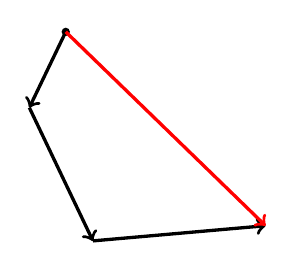
\begin{tikzpicture}[scale=0.5]
      \fill (0,0,0) circle[radius=3pt];
      \draw[->,very thick] (0,0,0) -- (1,0,5);
      \draw[->,very thick] (1,0,5) -- (3,-3,6);
      \draw[->,very thick] (3,-3,6) -- (7,-3,5);
      \draw[->,very thick,color=red] (0,0,0) -- (7,-3,5);
    \end{tikzpicture}
  \end{gather*}
  \item
  \begin{gather*}
    \vv{e} = \vv{a} - \vv{b} = \vv{a} + (-\vv{b}) \text{ (Gegenvektor von $\vv{b}$)} \\
    \vv{e} = \begin{pmatrix}1 \\ 0 \\ 5\end{pmatrix} - \begin{pmatrix}2 \\ -3 \\ 1\end{pmatrix} = \begin{pmatrix}1 \\ 0 \\ 5\end{pmatrix} + \begin{pmatrix}-2 \\ 3 \\ -1\end{pmatrix} = \begin{pmatrix}-1 \\ 3 \\ 4\end{pmatrix}
  \end{gather*}
  \begin{gather*}
    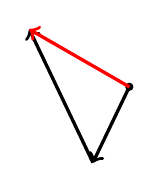
\begin{tikzpicture}[scale=0.5]
      \fill (0,0,0) circle[radius=3pt];
      \draw[->,very thick] (0,0,0) -- (1,0,5);
      \draw[->,very thick] (1,0,5) -- (-1,3,4);
      \draw[->,very thick,color=red] (0,0,0) -- (-1,3,4);
    \end{tikzpicture}
  \end{gather*}
  \item
  \begin{gather*}
    \vv{f} = 3 \cdot \vv{a} \\
    \vv{f} = 3 \cdot \begin{pmatrix}1 \\ 0 \\ 5\end{pmatrix} = \begin{pmatrix}3 \\ 0 \\ 15\end{pmatrix}
  \end{gather*}
\end{itemize}
\subsubsection{Darstellung eines Vektors durch andere Vektoren (Bsp. Verbindungsvektor)}
\begin{gather*}
  \vv{a} = \vv{OA} = \begin{pmatrix}4 \\ 4 \\ 1\end{pmatrix} \qquad \vv{b} = \vv{OB} = \begin{pmatrix}-1 \\ 0 \\ 3\end{pmatrix} \\
  \vv{AB} = -\vv{a} + \vv{b} = -\vv{OA} + \vv{OB} = \vv{OB} - \vv{OA} = \begin{pmatrix}-1 \\ 0 \\ 3\end{pmatrix} - \begin{pmatrix}4 \\ 4 \\ 1\end{pmatrix} = \begin{pmatrix}-5 \\ -4 \\ 2\end{pmatrix}
\end{gather*}
\begin{exercise}{279/6}
  \item [a]
  \begin{gather*}
    A(-2|2|3) \qquad B(5|5|5) \qquad C(9|6|5) \qquad D(2|3|3) \\
    \vv{AB} = \begin{pmatrix}7 \\ 3 \\ 2\end{pmatrix} \qquad \vv{DC} = \begin{pmatrix}7 \\ 3 \\ 2\end{pmatrix} \\
    \vv{AB} = \vv{DC} \quad\Rightarrow\quad \text{Parallelogramm}
  \end{gather*}
  \item [b]
  \begin{gather*}
    A(2|0|3) \qquad B(4|4|4) \qquad C(11|7|9) \qquad D(9|3|8) \\
    \vv{AB} = \begin{pmatrix}2 \\ 4 \\ 1\end{pmatrix} \qquad \vv{DC} = \begin{pmatrix}2 \\ 4 \\ 1\end{pmatrix} \\
    \vv{AB} = \vv{DC} \quad\Rightarrow\quad \text{Parallelogramm}
  \end{gather*}
  \item [c]
  \begin{gather*}
    A(2|-2|7) \qquad B(6|5|1) \qquad C(1|-1|1) \qquad D(8|0|8) \\
    \vv{AB} = \begin{pmatrix}4 \\ 7 \\ -6\end{pmatrix} \qquad \vv{DC} = \begin{pmatrix}-7 \\ -1 \\ -7\end{pmatrix} \\
    \vv{AB} \neq \vv{DC} \quad\Rightarrow\quad \text{kein Parallelogramm}
  \end{gather*}
\end{exercise}
\newpage
\begin{exercise}{279/7}
  \item [a]
  \begin{gather*}
    A(21|-11|43) \qquad B(3|7|-8) \qquad C(0|4|5) \\
  \vv{AB} = \begin{pmatrix}-18 \\ 18 \\ -51\end{pmatrix} \qquad \vv{BC} = \begin{pmatrix}-3 \\ -3 \\ 13\end{pmatrix} \\
  \vv{OD_1} = \vv{OA} + \vv{BC} = \begin{pmatrix}18 \\ -14 \\ 56\end{pmatrix} \\
  \vv{OD_2} = \vv{OC} + \vv{AB} = \begin{pmatrix}-18 \\ 22 \\ -46\end{pmatrix} \\
  \vv{OD_3} = \vv{OA} - \vv{BC} = \begin{pmatrix}24 \\ -8 \\ 30\end{pmatrix}
  \end{gather*}
  \begin{gather*}
    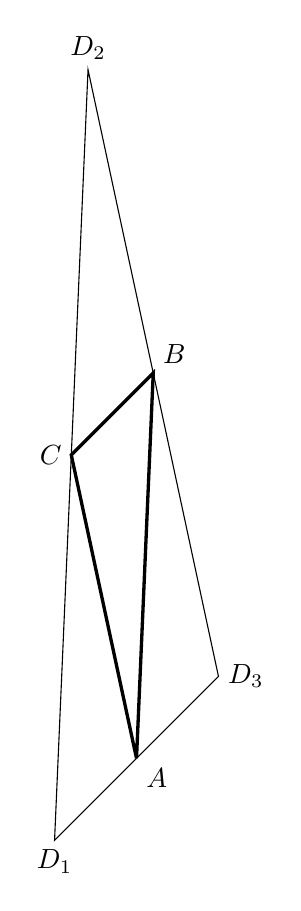
\begin{tikzpicture}[scale=0.13]
      \coordinate (A) at (21,-11,43);
      \coordinate (B) at (3,7,-8);
      \coordinate (C) at (0,4,5);
      \coordinate (D1) at (18,-14,56);
      \coordinate (D2) at (-18,22,-46);
      \coordinate (D3) at (24,-8,30);
      \node[below right] at (A) {$A$};
      \node[above right] at (B) {$B$};
      \node[left] at (C) {$C$};
      \node[below] at (D1) {$D_1$};
      \node[above] at (D2) {$D_2$};
      \node[right] at (D3) {$D_3$};
      \draw[very thick] (A) -- (B) -- (C) -- (A);
      \draw (A) -- (D1) -- (C);
      \draw (B) -- (D2) -- (C);
      \draw (A) -- (D3) -- (B);
    \end{tikzpicture}
  \end{gather*}
  \item [b]
  \begin{gather*}
    A(-75|199|-67) \qquad B(35|0|-81) \qquad C(1|2|3) \\
    \vv{AB} = \begin{pmatrix}110 \\ -199 \\ 14\end{pmatrix} \qquad \vv{BC} = \begin{pmatrix}-34 \\ 2 \\ 84\end{pmatrix} \\
    \vv{OD_1} = \vv{OA} + \vv{BC} = \begin{pmatrix}-109 \\ 201 \\ 17\end{pmatrix} \\
    \vv{OD_2} = \vv{OC} + \vv{AB} = \begin{pmatrix}111 \\ -197 \\ 17\end{pmatrix} \\
    \vv{OD_3} = \vv{OA} - \vv{BC} = \begin{pmatrix}-41 \\ 197 \\ -151\end{pmatrix}
  \end{gather*}
  \begin{gather*}
    \begin{tikzpicture}[scale=0.024]
      \coordinate (A) at (-75,199,-67);
      \coordinate (B) at (35,0,-81);
      \coordinate (C) at (1,2,3);
      \coordinate (D1) at (-109,201,17);
      \coordinate (D2) at (111,-197,17);
      \coordinate (D3) at (-41,197,-151);
      \node[above left] at (A) {$A$};
      \node[right] at (B) {$B$};
      \node[below left] at (C) {$C$};
      \node[left] at (D1) {$D_1$};
      \node[below right] at (D2) {$D_2$};
      \node[above right] at (D3) {$D_3$};
      \draw[very thick] (A) -- (B) -- (C) -- (A);
      \draw (A) -- (D1) -- (C);
      \draw (B) -- (D2) -- (C);
      \draw (A) -- (D3) -- (B);
    \end{tikzpicture}
  \end{gather*}
\end{exercise}
\subsection{Vektorzüge und Linearkombinationen}
(zu 279/6) \\\\
$M_1$ ... Mittelpunkt von $\overline{AB}$ \\
$M_2$ ... Mittelpunkt des Parallelogramms (mit $D_1$)
\begin{gather*}
  \vv{OM_1} = \vv{OA} + \frac{1}{2} \cdot \vv{AB} = \vv{OB} - \frac{1}{2}\vv{AB} \\
  \vv{OM_2} = \vv{OA} + \frac{1}{2} \cdot \vv{AC} = \vv{OC} - \frac{1}{2}\vv{AC}
\end{gather*}
\begin{itemize}
  \item [zu 6a]
  \begin{gather*}
    \vv{OA} = \begin{pmatrix}-2 \\ 2 \\ 3\end{pmatrix} \qquad \vv{OB} = \begin{pmatrix}5 \\ 5 \\ 5\end{pmatrix} \qquad \vv{OC} = \begin{pmatrix}9 \\ 6 \\ 5\end{pmatrix} \\
    \vv{OM_1} = \begin{pmatrix}-2 \\ 2 \\ 3\end{pmatrix} + \frac{1}{2} \cdot \begin{pmatrix}7 \\ 3 \\ 2\end{pmatrix} = \begin{pmatrix}1.5 \\ 3.5 \\ 4\end{pmatrix} \\
    \vv{OM_2} = \begin{pmatrix}-2 \\ 2 \\ 3\end{pmatrix} + \frac{1}{2} \cdot \begin{pmatrix}11 \\ 4 \\ 2\end{pmatrix} = \begin{pmatrix}3.5 \\ 4 \\ 4\end{pmatrix}
  \end{gather*}
  \item [zu 6b]
  \begin{gather*}
    \vv{OA} = \begin{pmatrix}2 \\ 0 \\ 3\end{pmatrix} \qquad \vv{OB} = \begin{pmatrix}4 \\ 4 \\ 4\end{pmatrix} \qquad \vv{OC} = \begin{pmatrix}11 \\ 7 \\ 9\end{pmatrix} \\
    \vv{OM_1} = \begin{pmatrix}2 \\ 0 \\ 3\end{pmatrix} + \frac{1}{2} \cdot \begin{pmatrix}2 \\ 4 \\ 1\end{pmatrix} = \begin{pmatrix}3 \\ 2 \\ 3.5\end{pmatrix} \\
    \vv{OM_2} = \begin{pmatrix}2 \\ 0 \\ 3\end{pmatrix} + \frac{1}{2} \cdot \begin{pmatrix}9 \\ 7 \\ 6\end{pmatrix} = \begin{pmatrix}6.5 \\ 3.5 \\ 6\end{pmatrix}
  \end{gather*}
\end{itemize}
Setze ich mehrere Vektorpfeile, mit Koeffizienten multipliziert, aneinander, so nennt man das einen Vektorzug. Die rechnerische Summe solcher Vektoren heißt Linearkombination.
\newpage
\begin{exercise}{283/5}
  \item [a]
  \begin{gather*}
    2 \cdot \begin{pmatrix}1 \\ 2\end{pmatrix} + 3 \cdot \begin{pmatrix}2 \\ 0\end{pmatrix} = \begin{pmatrix}8 \\ 4\end{pmatrix}
  \end{gather*}
  \begin{gather*}
    \begin{tikzpicture}
      \draw[->] (0,0) -- (1,2);
      \draw[->] (1,2) -- (2,4);
      \draw[->] (2,4) -- (4,4);
      \draw[->] (4,4) -- (6,4);
      \draw[->] (6,4) -- (8,4);
      \draw[->] (0,0) -- (2,0);
      \draw[->] (2,0) -- (4,0);
      \draw[->] (4,0) -- (6,0);
      \draw[->] (6,0) -- (7,2);
      \draw[->] (7,2) -- (8,4);
      \draw[->,color=red] (0,0) -- (8,4);
    \end{tikzpicture}
  \end{gather*}
  \item [b]
  \begin{gather*}
    4 \cdot \begin{pmatrix}1 \\ 1\end{pmatrix} - 2 \cdot \begin{pmatrix}1 \\ 3\end{pmatrix} = \begin{pmatrix}2 \\ -2\end{pmatrix}
  \end{gather*}
  \begin{gather*}
    \begin{tikzpicture}
      \draw[->] (0,0) -- (1,1);
      \draw[->] (1,1) -- (2,2);
      \draw[->] (2,2) -- (3,3);
      \draw[->] (3,3) -- (4,4);
      \draw[->] (4,4) -- (3,1);
      \draw[->] (3,1) -- (2,-2);
      \draw[->] (0,0) -- (-1,-3);
      \draw[->] (-1,-3) -- (-2,-6);
      \draw[->] (-2,-6) -- (-1,-5);
      \draw[->] (-1,-5) -- (0,-4);
      \draw[->] (0,-4) -- (1,-3);
      \draw[->] (1,-3) -- (2,-2);
      \draw[->,color=red] (0,0) -- (2,-2);
    \end{tikzpicture}
  \end{gather*}
  \item [c]
  \begin{gather*}
  3 \cdot \begin{pmatrix}-1 \\ -2\end{pmatrix} + 2 \cdot \begin{pmatrix}1 \\ -3\end{pmatrix} = \begin{pmatrix}-1 \\ -12\end{pmatrix}
  \end{gather*}
  \begin{gather*}
    \begin{tikzpicture}
      \draw[->] (0,0) -- (-1,-2);
      \draw[->] (-1,-2) -- (-2,-4);
      \draw[->] (-2,-4) -- (-3,-6);
      \draw[->] (-3,-6) -- (-2,-9);
      \draw[->] (-2,-9) -- (-1,-12);
      \draw[->] (0,0) -- (1,-3);
      \draw[->] (1,-3) -- (2,-6);
      \draw[->] (2,-6) -- (1,-8);
      \draw[->] (1,-8) -- (0,-10);
      \draw[->] (0,-10) -- (-1,-12);
      \draw[->,color=red] (0,0) -- (-1,-12);
    \end{tikzpicture}
  \end{gather*}
\end{exercise}
\begin{exercise}{283/7}
  \item [d]
  \begin{gather*}
    \begin{pmatrix}5 \\ 6 \\ 7\end{pmatrix} + (-1) \cdot \begin{pmatrix}0 \\ 2 \\ 4\end{pmatrix} = \begin{pmatrix}5 \\ 4 \\ 3\end{pmatrix}
  \end{gather*}
  \item [e]
  \begin{gather*}
    3 \cdot \begin{pmatrix}-1 \\ 4 \\ 2\end{pmatrix} - 2 \cdot \begin{pmatrix}-2 \\ 4 \\ 1\end{pmatrix} + 3 \cdot \begin{pmatrix}-1 \\ 4 \\ 2\end{pmatrix} = \begin{pmatrix}-2 \\ 16 \\ 10\end{pmatrix}
  \end{gather*}
  \item [f]
  \begin{gather*}
    4 \cdot \begin{pmatrix}0.5 \\ 3 \\ 1\end{pmatrix} + 2 \cdot \begin{pmatrix}1 \\ 6 \\ 2\end{pmatrix} + 3 \cdot \begin{pmatrix}0.8 \\ 2 \\ 3\end{pmatrix} = \begin{pmatrix}6.4 \\ 30 \\ 17\end{pmatrix}
  \end{gather*}
\end{exercise}
\begin{exercise}{284/11}
  \item [f] $-(\vv{u} - \vv{v}) = \vv{v} - \vv{u}$
  \item [g] $2(2\vv{a} + 4\vv{b}) = 4\vv{a} + 8\vv{b}$
  \item [h] $-4(\vv{a} - \vv{b}) - \vv{b} + \vv{a} = 3\vv{a} - 3\vv{b}$
  \item [i] $3(\vv{a} + 2(\vv{a} + \vv{b})) = 9\vv{a} + 6\vv{b}$
  \item [j] $6(\vv{a} - \vv{b}) + 4(\vv{a} + \vv{b}) = 10\vv{a} - 2\vv{b}$
  \item [k] $7\vv{u} + 5(\vv{u} - 2(\vv{u} + \vv{v})) = 2\vv{u} - 10\vv{v}$
\end{exercise}
\begin{exercise}{284/12}
  \item [a] $\vv{AG} = \vv{a} + \vv{b} + \vv{c}$
  \item [b] $\vv{BH} = -\vv{a} + \vv{b} + \vv{c}$
  \item [c] $\vv{EC} = \vv{a} + \vv{b} - \vv{c}$
  \item [d] $\vv{ME} = -\frac{1}{2}\vv{a} - \frac{1}{2}\vv{b} + \vv{c}$
\end{exercise}
\section{Geraden in $\mathbb{R}^3$}
\begin{gather*}
  \begin{tikzpicture}
    \coordinate (O) at (0,0,0);
    \coordinate (A) at (-1,0,3);
    \coordinate (B) at (3,0,3);
    \coordinate (S1) at (1,0,3);
    \coordinate (S2) at (0,0,3);
    \coordinate (S3) at (2,0,3);
    \coordinate (S4) at (5,0,3);
    \coordinate (S5) at (-2,0,3);
    \node[above] at (O) {$O$};
    \node[above] at (A) {$A$};
    \node[above] at (B) {$B$};
    \node[above] at (S1) {$S_1$};
    \node[above] at (S2) {$S_2$};
    \node[above] at (S3) {$S_3$};
    \node[above] at (S4) {$S_4$};
    \node[above] at (S5) {$S_5$};
    \fill (O) circle[radius=1pt];
    \fill (A) circle[radius=1pt];
    \fill (B) circle[radius=1pt];
    \fill (S1) circle[radius=1pt];
    \fill (S2) circle[radius=1pt];
    \fill (S3) circle[radius=1pt];
    \fill (S4) circle[radius=1pt];
    \fill (S5) circle[radius=1pt];
    \draw (A) -- (B);
  \end{tikzpicture}
\end{gather*}
\begin{gather*}
  \vv{OS_1} = \vv{OA} + \frac{1}{2}\vv{AB} \\
  \vv{OS_2} = \vv{OA} + \frac{1}{4}\vv{AB} \\
  \vv{OS_3} = \vv{OA} + \frac{3}{4}\vv{AB} \\
  \vv{OS_4} = \vv{OA} + \frac{3}{2}\vv{AB} = \vv{OB} + \frac{1}{2}\vv{AB} \\
  \vv{OS_5} = \vv{OA} - \frac{1}{4}\vv{AB}
\end{gather*}
Gerade durch die Punkte $A$ und $B$:
\begin{gather*}
  g \colon \vv{x} = \vv{OA} + s \cdot \vv{AB} \qquad s \in \mathbb{R}
\end{gather*}
Parametergleichung einer Geraden $g$:
\begin{itemize}
  \item [$g$] Name der Geraden
  \item [$\vv{x}$] Ortsvektor eines unbestimmten Punktes
  \item [$\vv{OA}$] Ortsvektor eines bestimmten Punktes $A$ (heißt auch Stützvektor)
  \item [$s$] Parameter $s \in \mathbb{R}$ \\
  Beim Durchlaufen aller Zahlen von $\mathbb{R}$ werden nacheinander alle Punkte der Geraden $g$ dargestellt
  \item [$\vv{AB}$] Richtungsvektor von $g$ gibt die Richtung von $g$ an
\end{itemize}
\begin{gather*}
  h \colon \vv{x} = \vv{a} + r \cdot \vv{b} \\
  h \colon \vv{x} = \begin{pmatrix}1 \\ 0 \\ 2\end{pmatrix} + r \cdot \begin{pmatrix}-3 \\ 5 \\ 2\end{pmatrix} \\\\
  \text{Beispiele für Punkte auf $h$} \\
  \vv{OP_1} = \begin{pmatrix}1 \\ 0 \\ 2\end{pmatrix} \qquad r = 0 \\
  \vv{OP_2} = \begin{pmatrix}-2 \\ 5 \\ 4\end{pmatrix} \qquad r = 1 \\
  \vv{OP_3} = \begin{pmatrix}-5 \\ 10 \\ 6\end{pmatrix} \qquad r = 2 \\
  \vv{OP_4} = \begin{pmatrix}4 \\ -5 \\ 0\end{pmatrix} \qquad r = -1
\end{gather*}
\begin{gather*}
  \vv{OQ} = \begin{pmatrix}3 \\ 7 \\ -1\end{pmatrix} \in h \\
  \begin{pmatrix}3 \\ 7 \\ -1\end{pmatrix} = \begin{pmatrix}1 \\ 0 \\ 2\end{pmatrix} + r \cdot \begin{pmatrix}-3 \\ 5 \\ 2\end{pmatrix} \\
  \text{gibt es ein $r$, das alle 3 Gleichungen löst?} \\
  3 = 1 - 3r \quad\Rightarrow\quad r = -\frac{2}{3} \\
  7 = 5r \quad\Rightarrow\quad r = \frac{7}{5} \\
  -1 = 2 + 2r \quad\Rightarrow\quad r = -\frac{3}{2} \\
  \Rightarrow\quad Q \notin h
\end{gather*}
\begin{exercise}{287/2}
  \item [a]
  \begin{gather*}
    A(1|2|2) \qquad B(5|-4|7) \\
    g \colon \vv{x} = \vv{OA} + s \cdot \vv{AB} = \begin{pmatrix}1 \\ 2 \\ 2\end{pmatrix} + s \cdot \begin{pmatrix}4 \\ -6 \\ 5\end{pmatrix} \\
    g \colon \vv{x} = \vv{OB} + s \cdot \vv{AB} = \begin{pmatrix}5 \\ -4 \\ 7\end{pmatrix} + s \cdot \begin{pmatrix}4 \\ -6 \\ 5\end{pmatrix}
  \end{gather*}
  \item [b]
  \begin{gather*}
    A(-3|-2|9) \qquad B(0|0|3) \\
    g \colon \vv{x} = \vv{OA} + s \cdot \vv{AB} = \begin{pmatrix}-3 \\ -2 \\ 9\end{pmatrix} + s \cdot \begin{pmatrix}3 \\ 2 \\ -6\end{pmatrix} \\
    g \colon \vv{x} = \vv{OB} + s \cdot \vv{AB} = \begin{pmatrix}0 \\ 0 \\ 3\end{pmatrix} + s \cdot \begin{pmatrix}3 \\ 2 \\ -6\end{pmatrix}
  \end{gather*}
  \item [c]
  \begin{gather*}
    A(7|-2|7) \qquad B(1|1|1) \\
    g \colon \vv{x} = \vv{OA} + s \cdot \vv{AB} = \begin{pmatrix}7 \\ -2 \\ 7\end{pmatrix} + s \cdot \begin{pmatrix}-6 \\ 3 \\ -6\end{pmatrix} \\
    g \colon \vv{x} = \vv{OB} + s \cdot \vv{AB} = \begin{pmatrix}1 \\ 1 \\ 1\end{pmatrix} + s \cdot \begin{pmatrix}-6 \\ 3 \\ -6\end{pmatrix}
  \end{gather*}
\end{exercise}
\begin{exercise}{287/3}
  \item [c]
  \begin{gather*}
    X(2|3|-1) \qquad g \colon \vv{x} = \begin{pmatrix}7 \\ 0 \\ 4\end{pmatrix} + t \cdot \begin{pmatrix}5 \\ -3 \\ 5\end{pmatrix} \\
    2 = 7 + t \cdot 5 \quad\Rightarrow\quad t = -1 \\
    3 = t \cdot -3 \quad\Rightarrow\quad t = -1 \\
    -1 = 4 + t \cdot 5 \quad\Rightarrow\quad t = -1 \\
    \Rightarrow\quad X \in g
  \end{gather*}
  \item [d]
  \begin{gather*}
    X(2|-1|-1) \qquad g \colon \vv{x} = \begin{pmatrix}1 \\ 0 \\ 1\end{pmatrix} + t \cdot \begin{pmatrix}1 \\ 3 \\ 3\end{pmatrix} \\
    2 = 1 + t \quad\Rightarrow\quad t = 1 \\
    -1 = t \cdot 3 \quad\Rightarrow\quad t = -\frac{1}{3} \\
    \Rightarrow\quad X \notin g
  \end{gather*}
\end{exercise}
\begin{exercise}{288/12}
  \item [a]
  \begin{itemize}
    \item [$g$]
    \begin{gather*}
      P_1(2|9|0) \qquad P_2(-4|1|0) \qquad g \colon \vv{x} = \begin{pmatrix}2 \\ 9 \\ 0\end{pmatrix} + t \cdot \begin{pmatrix}3 \\ 4 \\ 0\end{pmatrix}
    \end{gather*}
    \item [$h$]
    \begin{gather*}
      H(-4|1|3) \qquad P(2|5|-3) \qquad h \colon \vv{x} = \begin{pmatrix}-4 \\ 1 \\ 3\end{pmatrix} + t \cdot \begin{pmatrix}3 \\ 2 \\ -3\end{pmatrix}
    \end{gather*}
    \item [$i$]
    \begin{gather*}
      P_1(-4|5|3) \qquad P_2(-4|9|0) \qquad i \colon \vv{x} = \begin{pmatrix}-4 \\ 5 \\ 3\end{pmatrix} + t \cdot \begin{pmatrix}0 \\ 4 \\ -3\end{pmatrix}
    \end{gather*}
    \item [$j$]
    \begin{gather*}
      P_1(-1|1|0) \qquad P_2(-1|5|3) \qquad j \colon \vv{x} = \begin{pmatrix}-1 \\ 1 \\ 0\end{pmatrix} + t \cdot \begin{pmatrix}0 \\ 4 \\ 3\end{pmatrix}
    \end{gather*}
  \end{itemize}
  \item [b]
  \begin{itemize}
    \item [$g$]
    \begin{gather*}
      C(-8|11|0) \qquad P(-2|5|3) \qquad g \colon \vv{x} = \begin{pmatrix}-8 \\ 11 \\ 0\end{pmatrix} + t \cdot \begin{pmatrix}2 \\ -2 \\ 1\end{pmatrix}
    \end{gather*}
    \item [$h$]
    \begin{gather*}
      P_1(-2|5|3) \qquad P_2(-6|9|3) \qquad h \colon \vv{x} = \begin{pmatrix}-2 \\ 5 \\ 3\end{pmatrix} + t \cdot \begin{pmatrix}-2 \\ 2 \\ 0\end{pmatrix}
    \end{gather*}
    \item [$i$]
    \begin{gather*}
      B(0|11|0) \qquad P(-6|5|3) \qquad i \colon \vv{x} = \begin{pmatrix}0 \\ 11 \\ 0\end{pmatrix} + t \cdot \begin{pmatrix}-2 \\ -2 \\ 1\end{pmatrix}
    \end{gather*}
    \item [$j$]
    \begin{gather*}
      M(-4|7|0) \qquad P(-6|5|3) \qquad j \colon \vv{x} = \begin{pmatrix}-4 \\ 7 \\ 0\end{pmatrix} + t \cdot \begin{pmatrix}-2 \\ -2 \\ 3\end{pmatrix}
    \end{gather*}
  \end{itemize}
\end{exercise}
\subsection{Kollinearität}
\begin{gather*}
  g \colon \vv{x} = \vv{a} + t \cdot \vv{b} \qquad t \in \mathbb{R} \\
  \text{für $\vv{b}$ gilt: $\vv{b}$ kann durch $\vv{b}' = s \cdot \vv{b}$ ersetzt werden} \qquad s \in \mathbb{R} \quad s \neq 0 \\
  \vv{b}' \parallel \vv{b} \qquad \text{$\vv{b}'$ und $\vv{b}$ sind kollinear}
\end{gather*}
Sonderfall: Gerade durch $O$
\begin{gather*}
  \text{z. B. } g \colon \vv{x} = t \cdot \begin{pmatrix}1 \\ 3 \\ 5\end{pmatrix} = \begin{pmatrix}-2 \\ -6 \\ -10\end{pmatrix} + s \cdot \begin{pmatrix}1 \\ 3 \\ 5\end{pmatrix} \\
  \text{hier ist $\vv{a} \parallel \vv{b}$, d. h. $\vv{a}$ und $\vv{b}$ sind kollinear ($\vv{a} = -2 \cdot \vv{b}$)}
\end{gather*}
\subsection{Lage zweier Geraden}
4 Möglichkeiten unterschiedlicher Lage:
\begin{itemize}
  \item Schnitt (Schnittpunkt)
  \item parallel
  \item identisch
  \item windschief
\end{itemize}
\subsubsection{Verfahren um festzustellen, welche Lage zwei Geraden $g$ und $h$ haben}
\begin{gather*}
  g \colon \vv{x} = \vv{a} + s \cdot \vv{b} \\
  h \colon \vv{x} = \vv{c} + t \cdot \vv{d}
\end{gather*}
\begin{gather*}
  \vv{b} \stackrel{?}{=} r \cdot \vv{d}
\end{gather*}
\begin{itemize}
  \item wahr:
  \begin{gather*}
    \vv{a} \stackrel{?}{=} \vv{c} + t \cdot \vv{d} \text{ oder } \vv{c} \stackrel{?}{=} \vv{a} + s \cdot \vv{b}
  \end{gather*}
  \begin{itemize}
    \item wenn wahr, dann sind $g$ und $h$ identisch
    \item wenn nicht wahr, dann sind $g$ und $h$ parallel
  \end{itemize}
  \newpage
  \item nicht wahr:
  \begin{gather*}
    \vv{a} + s \cdot \vv{b} = \vv{c} + t \cdot \vv{d}
  \end{gather*}
  \begin{itemize}
    \item finde ich ein $s$ und ein $t$, sodass das LGS gelöst wird, so schneiden sich $g$ und $h$ in einem Punkt $S$
    \item ansonsten sind $g$ und $h$ windschief
  \end{itemize}
\end{itemize}
\begin{exercise}{292/1}
  \item [a]
  \begin{gather*}
    g \colon \vv{x} = \begin{pmatrix}1 \\ 2 \\ 3\end{pmatrix} + r \cdot \begin{pmatrix}2 \\ 4 \\ 1\end{pmatrix} \\
    h \colon \vv{x} = \begin{pmatrix}3 \\ 6 \\ 4\end{pmatrix} + t \cdot \begin{pmatrix}4 \\ 8 \\ 2\end{pmatrix} \\\\
    \begin{pmatrix}2 \\ 4 \\ 1\end{pmatrix} = r \cdot \begin{pmatrix}4 \\ 8 \\ 2\end{pmatrix} \\
    r = 2 \\
    \Rightarrow \text{identisch oder parallel} \\\\
    \begin{pmatrix}1 \\ 2 \\ 3\end{pmatrix} = \begin{pmatrix}3 \\ 6 \\ 4\end{pmatrix} + t \cdot \begin{pmatrix}4 \\ 8 \\ 2\end{pmatrix} \\
    t = -\frac{1}{2} \\
    \Rightarrow \text{identisch}
  \end{gather*}
\end{exercise}
\newpage
\begin{exercise}{292/2}
  \item [a]
  \begin{gather*}
    g \colon \vv{x} = \begin{pmatrix}9 \\ 0 \\ 6\end{pmatrix} + r \cdot \begin{pmatrix}3 \\ 2 \\ 1\end{pmatrix} \\
    h \colon \vv{x} = \begin{pmatrix}7 \\ -2 \\ 2\end{pmatrix} + s \cdot \begin{pmatrix}1 \\ 1 \\ 2\end{pmatrix} \\\\
    \begin{pmatrix}9 \\ 0 \\ 6\end{pmatrix} + r \cdot \begin{pmatrix}3 \\ 2 \\ 1\end{pmatrix} = \begin{pmatrix}7 \\ -2 \\ 2\end{pmatrix} + s \cdot \begin{pmatrix}1 \\ 1 \\ 2\end{pmatrix} \\\\
    9 + 3r = 7 + s \\
    2r = -2 + s \\
    6 + r = 2 + 2s \\
    \Rightarrow \qquad r = 0 \qquad s = 2 \\\\
    \vv{OS} = \begin{pmatrix}9 \\ 0 \\ 6\end{pmatrix} + 0 \cdot \begin{pmatrix}3 \\ 2 \\ 1\end{pmatrix} = \begin{pmatrix}7 \\ -2 \\ 2\end{pmatrix} + 2 \cdot \begin{pmatrix}1 \\ 1 \\ 2\end{pmatrix} = \begin{pmatrix}9 \\ 0 \\ 6\end{pmatrix} \\\\
    S(9|0|6)
  \end{gather*}
\end{exercise}
\newpage
\begin{exercise}{292/4}
  \item [a]
  \begin{gather*}
    g \colon \vv{x} = \begin{pmatrix}5 \\ 0 \\ 1\end{pmatrix} + t \cdot \begin{pmatrix}2 \\ 1 \\ -1\end{pmatrix} \\
    h \colon \vv{x} = \begin{pmatrix}7 \\ 1 \\ 2\end{pmatrix} + t \cdot \begin{pmatrix}-6 \\ -3 \\ 3\end{pmatrix} \\\\
    \begin{pmatrix}2 \\ 1 \\ -1\end{pmatrix} = r \cdot \begin{pmatrix}-6 \\ -3 \\ 3\end{pmatrix} \\
    r = -3 \\
    \Rightarrow \text{identisch oder parallel} \\\\
    \begin{pmatrix}5 \\ 0 \\ 1\end{pmatrix} = \begin{pmatrix}7 \\ 1 \\ 2\end{pmatrix} + t \cdot \begin{pmatrix}-6 \\ -3 \\ 3\end{pmatrix} \\
    5 = 7 + t \cdot (-6) \quad\Rightarrow\quad t = \frac{1}{3} \\
    0 = 1 + t \cdot (-3) \quad\Rightarrow\quad t = \frac{1}{3} \\
    1 = 2 + t \cdot 3 \quad\Rightarrow\quad t = -\frac{1}{3} \\
    \Rightarrow \text{parallel}
  \end{gather*}
  \item [b]
  \begin{gather*}
    g \colon \vv{x} = t \cdot \begin{pmatrix}2 \\ 0 \\ 1\end{pmatrix} \\
    h \colon \vv{x} = \begin{pmatrix}2 \\ 3 \\ 4\end{pmatrix} + t \cdot \begin{pmatrix}0 \\ 1 \\ -1\end{pmatrix} \\\\
    \begin{pmatrix}2 \\ 0 \\ 1\end{pmatrix} \neq r \cdot \begin{pmatrix}0 \\ 1 \\ -1\end{pmatrix} \\
    \Rightarrow \text{nicht parallel} \\\\
    t_g \cdot \begin{pmatrix}2 \\ 0 \\ 1\end{pmatrix} = \begin{pmatrix}2 \\ 3 \\ 4\end{pmatrix} + t_h \cdot \begin{pmatrix}0 \\ 1 \\ -1\end{pmatrix} \\
    t_g \cdot 2 = 2 + t_h \cdot 0 \quad\Rightarrow\quad t_g = 1 \\
    t_g \cdot 0 = 3 + t_h \cdot 1 \quad\Rightarrow\quad t_h = -1 \\
    t_g \cdot 1 \neq 4 + t_h \cdot (-1) \\
    \Rightarrow \text{windschief}
  \end{gather*}
\end{exercise}
\begin{exercise}{293/8}
  \item [b]
  \begin{gather*}
    g \colon \vv{x} = \begin{pmatrix}2 \\ 2 \\ 1\end{pmatrix} + t \cdot \begin{pmatrix}1 \\ 2 \\ 0\end{pmatrix} \\
    h \colon \vv{x} = \begin{pmatrix}2 \\ 2 \\ 1\end{pmatrix} + t \cdot \begin{pmatrix}1 \\ 2 \\ 3\end{pmatrix} \\
    i \colon \vv{x} = t \cdot \begin{pmatrix}1 \\ 2 \\ 0\end{pmatrix} \\
    j \colon \vv{x} = t \cdot \begin{pmatrix}1 \\ 2 \\ 3\end{pmatrix}
  \end{gather*}
\end{exercise}
\subsection{Parameterpunkte und -geraden}
\begin{gather*}
  \vv{OA_b} = \begin{pmatrix}1 \\ 5 \\ b\end{pmatrix} = \begin{pmatrix}1 + b \cdot 0 \\ 5 + b \cdot 0 \\ 0 + b \cdot 1\end{pmatrix} = \begin{pmatrix}1 \\ 5 \\ 0\end{pmatrix} + b \cdot \begin{pmatrix}0 \\ 0 \\ 1\end{pmatrix} \\
  \vv{OC_d} = \begin{pmatrix}2d \\ 1 - 5d \\ 7\end{pmatrix} = \begin{pmatrix}0 + d \cdot 2 \\ 1 + d \cdot (-5) \\ 7 + d \cdot 0\end{pmatrix} = \begin{pmatrix}0 \\ 1 \\ 7\end{pmatrix} + d \cdot \begin{pmatrix}2 \\ -5 \\ 0\end{pmatrix}
\end{gather*}
\begin{gather*}
  g_a \colon \vv{x} = \begin{pmatrix}2 \\ a \\ 5\end{pmatrix} + r \begin{pmatrix}1 \\ 2 \\ 0\end{pmatrix} = \begin{pmatrix}2 \\ 0 \\ 5\end{pmatrix} + a \cdot \begin{pmatrix}0 \\ 1 \\ 0\end{pmatrix} + r \cdot \begin{pmatrix}1 \\ 2 \\ 0\end{pmatrix}
\end{gather*}
\begin{exercise}{293/10}
  \item [a]
  \begin{gather*}
    g_a \colon \vv{x} = \begin{pmatrix}3 \\ a \\ 3\end{pmatrix} + r \cdot \begin{pmatrix}-1 \\ 5 \\ 7\end{pmatrix} \qquad h_a \colon \vv{x} = \begin{pmatrix}1 \\ 0 \\ a\end{pmatrix} + s \cdot \begin{pmatrix}2 \\ -22 \\ -29\end{pmatrix} \\\\
    \begin{pmatrix}-1 \\ 5 \\ 7\end{pmatrix} \neq t \cdot \begin{pmatrix}2 \\ -22 \\ -29\end{pmatrix} \\
    \Rightarrow \text{nicht parallel} \\\\
    \begin{pmatrix}3 \\ a \\ 3\end{pmatrix} + r \cdot \begin{pmatrix}-1 \\ 5 \\ 7\end{pmatrix} = \begin{pmatrix}1 \\ 0 \\ a\end{pmatrix} + s \cdot \begin{pmatrix}2 \\ -22 \\ -29\end{pmatrix} \\
    3 - r = 1 + 2s \\
    a + 5r = -22s \\
    3 + 7r = a - 29s \\
    a = 2 \qquad r = 4 \qquad s = -1 \\\\
    \vv{OS} = \begin{pmatrix}3 \\ 2 \\ 3\end{pmatrix} + 4 \cdot \begin{pmatrix}-1 \\ 5 \\ 7\end{pmatrix} = \begin{pmatrix}-1 \\ 22 \\ 31\end{pmatrix}
  \end{gather*}
  \item [b]
  \begin{gather*}
    g_a \colon \vv{x} = \begin{pmatrix}3 \\ 2 \\ a\end{pmatrix} + r \cdot \begin{pmatrix}10 \\ 7 \\ 0\end{pmatrix} \qquad h_a \colon \vv{x} = \begin{pmatrix}a \\ -1 \\ 3\end{pmatrix} + s \cdot \begin{pmatrix}6 \\ 2 \\ -1\end{pmatrix} \\\\
    \begin{pmatrix}10 \\ 7 \\ 0\end{pmatrix} \neq t \cdot \begin{pmatrix}6 \\ 2 \\ -1\end{pmatrix} \\
    \Rightarrow \text{nicht parallel} \\\\
    \begin{pmatrix}3 \\ 2 \\ a\end{pmatrix} + r \cdot \begin{pmatrix}10 \\ 7 \\ 0\end{pmatrix} = \begin{pmatrix}a \\ -1 \\ 3\end{pmatrix} + s \cdot \begin{pmatrix}6 \\ 2 \\ -1\end{pmatrix} \\
    3 + 10r = a + 6s \\
    2 + 7r = -1 + 2s \\
    a = 3 - s \\
    a = 5 \qquad r = -1 \qquad s = -2 \\\\
    \vv{OS} = \begin{pmatrix}3 \\ 2 \\ 5\end{pmatrix} - \begin{pmatrix}10 \\ 7 \\ 0\end{pmatrix} = \begin{pmatrix}-7 \\ -5 \\ 5\end{pmatrix}
  \end{gather*}
\end{exercise}
\begin{exercise}{293/16}
  \begin{gather*}
    G = 10cm^2 \qquad h = 15cm \\
    V_Z = G \cdot h = 150cm^3 \\
    V_K = \frac{1}{3} \cdot G \cdot h = 50cm^3 \\
    V_Z - V_K = 100cm^3 = 0.1L
  \end{gather*}
\end{exercise}
\section{Abstand zweier Punkte, Vektorlänge, Streckenlänge}
\begin{gather*}
  \text{Bsp. } g \colon \vv{x} = \begin{pmatrix}1 \\ 2 \\ 3\end{pmatrix} + r \cdot \begin{pmatrix}2 \\ -1 \\ 0\end{pmatrix} \qquad r \in \mathbb{R} \colon \left[2;5\right]
\end{gather*}
\begin{gather*}
  \begin{tikzpicture}[scale=0.5]
    \coordinate (O) at (0,0,0);
    \coordinate (A) at (1,2,3);
    \coordinate (C) at (5,0,3);
    \coordinate (D) at (11,-3,3);
    \node[below] at (O) {$O$};
    \node[above right] at (A) {$A$};
    \node[above right] at (C) {$C$};
    \node[above right] at (D) {$D$};
    \fill (O) circle[radius=2pt];
    \fill (A) circle[radius=2pt];
    \draw[->] (O) -- (A);
    \draw (-3,4,3) -- (15,-5,3);
    \draw[red,very thick] (C) -- (D);
  \end{tikzpicture}
\end{gather*}
\begin{gather*}
  \vv{OC} = \begin{pmatrix}5 \\ 0 \\ 3\end{pmatrix} \qquad \vv{OD} = \begin{pmatrix}11 \\ -3 \\ 3\end{pmatrix} \\
  |\overline{CD}| = |\vv{CD}| = \text{Abstand } C \leftrightarrow D \\
  \vv{CD} = \begin{pmatrix}6 \\ -3 \\ 0\end{pmatrix}
\end{gather*}
\begin{gather*}
  \textbf{Seitenlängen des Segels (Bsp. S. 294)} \\
  \text{unten} \colon 4m \\
  \text{links} \colon \sqrt{(5m)^2 + (3m)^2} \quad\text{(Satz des Pythagoras)} \\
  \text{rechts} \colon \sqrt{(\sqrt{34}m)^2 + (4m)^2} = \sqrt{(5m)^2 + (3m)^2 + (4m)^2}
\end{gather*}
\begin{gather*}
  |\vv{CD}| = \sqrt{6^2 + (-3)^2 + 0^2} = \sqrt{45} \approx 6.71LE
\end{gather*}
Die Länge eines Vektors $\begin{pmatrix}a \\ b \\ c\end{pmatrix}$ ist $\left|\begin{pmatrix}a \\ b \\ c\end{pmatrix}\right| = \sqrt{a^2 + b^2 + c^2}$
\begin{exercise}{297/2}
  \item [a]
  \begin{gather*}
    A(0|0|0) \qquad B(2|3|-1) \\
    \vv{AB} = \begin{pmatrix}2 \\ 3 \\ -1\end{pmatrix} \\
    |\vv{AB}| = \sqrt{2^2 + 3^2 + (-1)^2} = \sqrt{14} \approx 3.74LE
  \end{gather*}
  \item [b]
  \begin{gather*}
    A(2|2|-2) \qquad B(0|-1|5) \\
    \vv{AB} = \begin{pmatrix}-2 \\ -3 \\ 7\end{pmatrix} \\
    |\vv{AB}| = \sqrt{(-2)^2 + (-3)^2 + 7^2} = \sqrt{62} \approx 7.87LE
  \end{gather*}
  \item [c]
  \begin{gather*}
    A(1|5|6) \qquad B(1|6|7) \\
    \vv{AB} = \begin{pmatrix}0 \\ 1 \\ 1\end{pmatrix} \\
    |\vv{AB}| = \sqrt{0^2 + 1^2 + 1^2} = \sqrt{2} \approx 1.41LE
  \end{gather*}
\end{exercise}
\subsection{Einheitsvektor}
Ein Einheitsvektor hat die Länge $1LE$ \\
Einheitsvektor zu z. B. $\vv{a} = \begin{pmatrix}2 \\ 5 \\ 1\end{pmatrix} \qquad |\vv{a}| = \sqrt{30}$
\begin{gather*}
  \vv{a_0} = \frac{1}{\sqrt{30}} \cdot \begin{pmatrix}2 \\ 5 \\ 1\end{pmatrix}
\end{gather*}
\begin{exercise}{297/8}
  \item [a]
  \begin{gather*}
    A(1|-2|2) \qquad B(3|2|1) \qquad C(3|0|3) \\
    \vv{AB} = \begin{pmatrix}2 \\ 4 \\ -1\end{pmatrix} \qquad |\vv{AB}| = \sqrt{2^2 + 4^2 + (-1)^2} = \sqrt{21} \\
    \vv{AC} = \begin{pmatrix}2 \\ 2 \\ 1\end{pmatrix} \qquad |\vv{AC}| = \sqrt{2^2 + 2^2 + 1^2} = \sqrt{9} \\
    \vv{BC} = \begin{pmatrix}0 \\ -2 \\ 2\end{pmatrix} \qquad |\vv{BC}| = \sqrt{0^2 + (-2)^2 + 2^2} = \sqrt{8} \\
    |\vv{AB}| \neq |\vv{AC}| \neq |\vv{BC}| \quad\Rightarrow\text{nicht gleichschenklig}
  \end{gather*}
  \item [b]
  \begin{gather*}
    A(7|0|-1) \qquad B(5|-3|-1) \qquad C(4|0|1) \\
    \vv{AB} = \begin{pmatrix}-2 \\ -3 \\ 0\end{pmatrix} \qquad |\vv{AB}| = \sqrt{(-2)^2 + (-3)^2 + 0^2} = \sqrt{13} \\
    \vv{AC} = \begin{pmatrix}-3 \\ 0 \\ 2\end{pmatrix} \qquad |\vv{AC}| = \sqrt{(-3)^2 + 0^2 + 2^2} = \sqrt{13} \\
    \vv{BC} = \begin{pmatrix}-1 \\ 3 \\ 2\end{pmatrix} \qquad |\vv{BC}| = \sqrt{(-1)^2 + 3^2 + 2^2} = \sqrt{14} \\
    |\vv{AB}| = |\vv{AC}| \quad\Rightarrow\text{gleichschenklig}
  \end{gather*}
\end{exercise}
\begin{exercise}{297/9}
  \item [a]
  \begin{gather*}
    A(4|2|-1) \qquad B(10|-8|9) \qquad C(4|0|1) \\
    \vv{OM_a} = \vv{OB} + \frac{1}{2} \cdot \vv{BC} = \begin{pmatrix}10 \\ -8 \\ 9\end{pmatrix} + \frac{1}{2} \cdot \begin{pmatrix}-6 \\ 8 \\ -8\end{pmatrix} = \begin{pmatrix}7 \\ -4 \\ 5\end{pmatrix} \\
    \vv{OM_b} = \vv{OC} + \frac{1}{2} \cdot \vv{CA} = \begin{pmatrix}4 \\ 0 \\ 1\end{pmatrix} + \frac{1}{2} \cdot \begin{pmatrix}0 \\ 2 \\ -2\end{pmatrix} = \begin{pmatrix}4 \\ 1 \\ 0\end{pmatrix} \\
    \vv{OM_c} = \vv{OA} + \frac{1}{2} \cdot \vv{AB} = \begin{pmatrix}4 \\ 2 \\ -1\end{pmatrix} + \frac{1}{2} \cdot \begin{pmatrix}6 \\ -10 \\ 10\end{pmatrix} = \begin{pmatrix}7 \\ -3 \\ 4\end{pmatrix} \\
    |\vv{AM_a}| = \left|\begin{pmatrix}3 \\ -6 \\ 6\end{pmatrix}\right| = \sqrt{3^2 + (-6)^2 + 6^2} = \sqrt{81} = 9 \\
    |\vv{BM_b}| = \left|\begin{pmatrix}-6 \\ 9 \\ -9\end{pmatrix}\right| = \sqrt{(-6)^2 + 9^2 + (-9)^2} = \sqrt{198} \approx 14.07 \\
    |\vv{CM_c}| = \left|\begin{pmatrix}3 \\ -3 \\ 3\end{pmatrix}\right| = \sqrt{3^2 + (-3)^2 + 3^2} = \sqrt{27} \approx 5.20
  \end{gather*}
  \item [b]
  \begin{gather*}
    A(1|2|-1) \qquad B(-1|10|15) \qquad C(9|6|-5) \\
    \vv{OM_a} = \vv{OB} + \frac{1}{2} \cdot \vv{BC} = \begin{pmatrix}-1 \\ 10 \\ 15\end{pmatrix} + \frac{1}{2} \cdot \begin{pmatrix}10 \\ -4 \\ -20\end{pmatrix} = \begin{pmatrix}4 \\ 8 \\ 5\end{pmatrix} \\
    \vv{OM_b} = \vv{OC} + \frac{1}{2} \cdot \vv{CA} = \begin{pmatrix}9 \\ 6 \\ -5\end{pmatrix} + \frac{1}{2} \cdot \begin{pmatrix}-8 \\ -4 \\ 4\end{pmatrix} = \begin{pmatrix}5 \\ 4 \\ -3\end{pmatrix} \\
    \vv{OM_c} = \vv{OA} + \frac{1}{2} \cdot \vv{AB} = \begin{pmatrix}1 \\ 2 \\ -1\end{pmatrix} + \frac{1}{2} \cdot \begin{pmatrix}-2 \\ 8 \\ 16\end{pmatrix} = \begin{pmatrix}0 \\ 6 \\ 7\end{pmatrix} \\
    |\vv{AM_a}| = \left|\begin{pmatrix}3 \\ 6 \\ 6\end{pmatrix}\right| = \sqrt{3^2 + 6^2 + 6^2} = \sqrt{81} = 9 \\
    |\vv{BM_b}| = \left|\begin{pmatrix}6 \\ -6 \\ -18\end{pmatrix}\right| = \sqrt{6^2 + (-6)^2 + (-18)^2} = \sqrt{396} \approx 19.90 \\
    |\vv{CM_c}| = \left|\begin{pmatrix}-9 \\ 0 \\ 12\end{pmatrix}\right| = \sqrt{(-9)^2 + 0^2 + 12^2} = \sqrt{225} = 15
  \end{gather*}
  \item [c]
  \begin{gather*}
    \text{zu a} \\
    |\vv{AS}| = \frac{2}{3} \cdot |\vv{AM_a}| = 6 \\
    |\vv{BS}| = \frac{2}{3} \cdot |\vv{BM_b}| \approx 9.38 \\
    |\vv{CS}| = \frac{2}{3} \cdot |\vv{CM_c}| \approx 3.46 \\\\
    \text{zu b} \\
    |\vv{AS}| = \frac{2}{3} \cdot |\vv{AM_a}| = 6 \\
    |\vv{BS}| = \frac{2}{3} \cdot |\vv{BM_b}| \approx 13.27 \\
    |\vv{CS}| = \frac{2}{3} \cdot |\vv{CM_c}| = 10
  \end{gather*}
\end{exercise}
\section{Produkte zweier Vektoren}
\subsection{Skalarprodukt}
Beispiel aus der Physik:
\begin{figure}[H]
  \centering
  \includegraphics[width=0.55\textwidth]{/fakepath/skalarprodukt_arbeit.png}
\end{figure}
\begin{gather*}
  W = \vv{F} \cdot \vv{s} \\
  cos(\alpha) = \frac{|\vv{F_s}|}{|\vv{F}|} \quad\Rightarrow\quad |\vv{F_s}| = |\vv{F}| \cdot cos(\alpha) \qquad \text{$\vv{F_s}$ ... $\vv{F}$ in Richtung $\vv{s}$} \\
  W = \vv{F} \cdot \vv{s} = |\vv{F}| \cdot cos(\alpha) \cdot |\vv{s}| \\\\
  \vv{a} \cdot \vv{b} = |\vv{a}| \cdot |\vv{b}| \cdot cos(\alpha) = a_1 \cdot b_1 + a_2 \cdot b_2 + a_3 \cdot b_3 \\
\end{gather*}
Beispiel:
\begin{gather*}
  \vv{a} = \begin{pmatrix}1 \\ 2 \\ 3\end{pmatrix} \qquad \vv{b} = \begin{pmatrix}-2 \\ 0 \\ 3\end{pmatrix} \\
  \vv{a} \cdot \vv{b} = 1 \cdot (-2) + 2 \cdot 0 + 3 \cdot 3 = 7 \\\\
  \text{Winkel zwischen $\vv{a}$ und $\vv{b}$:} \\
  7 = \left|\begin{pmatrix}1 \\ 2 \\ 3\end{pmatrix}\right| \cdot \left|\begin{pmatrix}-2 \\ 0 \\ 3\end{pmatrix}\right| \cdot cos(\alpha) = \sqrt{14} \cdot \sqrt{13} \cdot cos(\alpha) \\
  \alpha = acos(\frac{7}{\sqrt{14} \cdot \sqrt{13}}) \approx 1.025 \approx 58.73^\circ
\end{gather*}
Spezialfall:
\begin{gather*}
  \alpha = 90^\circ \\
  \Rightarrow cos(\alpha) = 0 \\
  \Rightarrow \vv{a} \cdot \vv{b} = 0 \\
  \vv{a} \perp \vv{b} \\\\
  \text{z. B. } \vv{a} = \begin{pmatrix}1 \\ -1 \\ 0\end{pmatrix} \qquad \vv{b} = \begin{pmatrix}3 \\ 3 \\ 5\end{pmatrix} \\
  \vv{a} \cdot \vv{b} = 1 \cdot 3 + (-1) \cdot 3 + 0 \cdot 5 = 0 \\
  \Rightarrow \vv{a} \perp \vv{b}
\end{gather*}
\begin{exercise}{321/1}
  \item [a]
  \begin{gather*}
    g \colon \vv{x} = \begin{pmatrix}2 \\ -2 \\ 0\end{pmatrix} + s \cdot \begin{pmatrix}-5 \\ 1 \\ 0\end{pmatrix} \qquad h \colon \vv{x} = \begin{pmatrix}5 \\ -1 \\ 0\end{pmatrix} + s \cdot \begin{pmatrix}-2 \\ 2 \\ 0\end{pmatrix} \\
    \begin{pmatrix}-5 \\ 1 \\ 0\end{pmatrix} \cdot \begin{pmatrix}-2 \\ 2 \\ 0\end{pmatrix} = 12 \\
    \Rightarrow g \notperp h
  \end{gather*}
  \item [b]
  \begin{gather*}
    g \colon \vv{x} = \begin{pmatrix}8 \\ 6 \\ -9\end{pmatrix} + s \cdot \begin{pmatrix}2 \\ -9 \\ -4\end{pmatrix} \qquad h \colon \vv{x} = \begin{pmatrix}0 \\ 0 \\ 7\end{pmatrix} + s \cdot \begin{pmatrix}5 \\ 2 \\ -2\end{pmatrix} \\
    \begin{pmatrix}2 \\ -9 \\ -4\end{pmatrix} \cdot \begin{pmatrix}5 \\ 2 \\ -2\end{pmatrix} = 0 \\
    \Rightarrow g \perp h
  \end{gather*}
\end{exercise}
\newpage
\begin{exercise}{zu 297/8}
  \item [a]
  \begin{gather*}
    \vv{AB} \cdot \vv{AC} = \begin{pmatrix}2 \\ 4 \\ -1\end{pmatrix} \cdot \begin{pmatrix}2 \\ 2 \\ 1\end{pmatrix} = 11 \qquad |\vv{AB}| \cdot |\vv{AC}| = \sqrt{21} \cdot \sqrt{9} \\
    \alpha = acos(\frac{11}{3\sqrt{21}}) \approx 0.64 \approx 36.86^\circ \\
    \vv{BA} \cdot \vv{BC} = \begin{pmatrix}-2 \\ -4 \\ 1\end{pmatrix} \cdot \begin{pmatrix}0 \\ -2 \\ 2\end{pmatrix} = 10 \qquad |\vv{BA}| \cdot |\vv{BC}| = \sqrt{21} \cdot \sqrt{8} \\
    \beta = acos(\frac{10}{\sqrt{21} \cdot \sqrt{8}}) \approx 0.69 \approx 39.51^\circ \\
    \vv{CA} \cdot \vv{CB} = \begin{pmatrix}-2 \\ -2 \\ -1\end{pmatrix} \cdot \begin{pmatrix}0 \\ 2 \\ -2\end{pmatrix} = -2 \qquad |\vv{CA}| \cdot |\vv{CB}| = \sqrt{9} \cdot \sqrt{8} \\
    \gamma = acos(\frac{-2}{3\sqrt{8}}) \approx 1.81 \approx 103.63^\circ
  \end{gather*}
  \item [b]
  \begin{gather*}
    \vv{AB} \cdot \vv{AC} = \begin{pmatrix}-2 \\ -3 \\ 0\end{pmatrix} \cdot \begin{pmatrix}-3 \\ 0 \\ 2\end{pmatrix} = 6 \qquad |\vv{AB}| \cdot |\vv{AC}| = \sqrt{13} \cdot \sqrt{13} \\
    \alpha = acos(\frac{6}{13}) \approx 1.09 \approx 62.51^\circ \\
    \vv{BA} \cdot \vv{BC} = \vv{CA} \cdot \vv{CB} = \begin{pmatrix}2 \\ 3 \\ 0\end{pmatrix} \cdot \begin{pmatrix}-1 \\ 3 \\ 2\end{pmatrix} = 7 \\
    |\vv{BA}| \cdot |\vv{BC}| = |\vv{CA}| \cdot |\vv{CB}| = \sqrt{13} \cdot \sqrt{14} \\
    \beta = \gamma = acos(\frac{7}{\sqrt{13} \cdot \sqrt{14}}) \approx 1.03 \approx 58.74^\circ
  \end{gather*}
\end{exercise}
\newpage
\begin{exercise}{zu 297/9}
  \item [a]
  \begin{gather*}
    \vv{AB} \cdot \vv{AC} = \begin{pmatrix}6 \\ -10 \\ 10\end{pmatrix} \cdot \begin{pmatrix}0 \\ -2 \\ 2\end{pmatrix} = 40 \qquad |\vv{AB}| \cdot |\vv{AC}| = \sqrt{236} \cdot \sqrt{8} \\
    \alpha = acos(\frac{40}{\sqrt{236} \cdot \sqrt{8}}) \approx 0.40 \approx 22.99^\circ \\
    \vv{BA} \cdot \vv{BC} = \begin{pmatrix}-6 \\ 10 \\ -10\end{pmatrix} \cdot \begin{pmatrix}-6 \\ 8 \\ -8\end{pmatrix} = 196 \qquad |\vv{BA}| \cdot |\vv{BC}| = \sqrt{236} \cdot \sqrt{164} \\
    \beta = acos(\frac{196}{\sqrt{236} \cdot \sqrt{164}}) \approx 0.09 \approx 4.95^\circ \\
    \vv{CA} \cdot \vv{CB} = \begin{pmatrix}0 \\ 2 \\ -2\end{pmatrix} \cdot \begin{pmatrix}6 \\ -8 \\ 8\end{pmatrix} = -32 \qquad |\vv{CA}| \cdot |\vv{CB}| = \sqrt{8} \cdot \sqrt{164} \\
    \gamma = acos(\frac{-32}{\sqrt{8} \cdot \sqrt{164}}) \approx 2.65 \approx 152.06^\circ
  \end{gather*}
  \item [b]
  \begin{gather*}
    \vv{AB} \cdot \vv{AC} = \begin{pmatrix}-2 \\ 8 \\ 16\end{pmatrix} \cdot \begin{pmatrix}8 \\ 4 \\ -4\end{pmatrix} = -48 \qquad |\vv{AB}| \cdot |\vv{AC}| = \sqrt{324} \cdot \sqrt{96} \\
    \alpha = acos(\frac{-48}{\sqrt{324} \cdot \sqrt{96}}) \approx 1.85 \approx 105.79^\circ \\
    \vv{BA} \cdot \vv{BC} = \begin{pmatrix}2 \\ -8 \\ -16\end{pmatrix} \cdot \begin{pmatrix}10 \\ -4 \\ -20\end{pmatrix} = 372 \qquad |\vv{BA}| \cdot |\vv{BC}| = \sqrt{324} \cdot \sqrt{516} \\
    \beta = acos(\frac{372}{\sqrt{324} \cdot \sqrt{516}}) \approx 0.43 \approx 24.52^\circ \\
    \vv{CA} \cdot \vv{CB} = \begin{pmatrix}-8 \\ -4 \\ 4\end{pmatrix} \cdot \begin{pmatrix}-10 \\ 4 \\ 20\end{pmatrix} = 144 \qquad |\vv{CA}| \cdot |\vv{CB}| = \sqrt{96} \cdot \sqrt{516} \\
    \gamma = acos(\frac{144}{\sqrt{96} \cdot \sqrt{516}}) \approx 0.87 \approx 49.68^\circ
  \end{gather*}
\end{exercise}
\newpage
\begin{exercise}{321/2}
  \item [a]
  \begin{gather*}
    \vv{a} = \begin{pmatrix}2 \\ 3 \\ 0\end{pmatrix} \qquad \vv{b} = \begin{pmatrix}b_1 \\ -4 \\ 3\end{pmatrix} \\
    \vv{a} \cdot \vv{b} = 0 \\
    2b_1 - 12 + 0 = 0 \quad\Rightarrow\quad b_1 = 6
  \end{gather*}
  \item [b]
  \begin{gather*}
    \vv{a} = \begin{pmatrix}1 \\ a_2 \\ 3\end{pmatrix} \qquad \vv{b} = \begin{pmatrix}2 \\ -1 \\ 1\end{pmatrix} \\
    \vv{a} \cdot \vv{b} = 0 \\
    2 - a_2 + 3 = 0 \quad\Rightarrow\quad a_2 = 5
  \end{gather*}
  \item [c]
  \begin{gather*}
    \vv{a} = \begin{pmatrix}-1 \\ 4 \\ 2\end{pmatrix} \qquad \vv{b} = \begin{pmatrix}3 \\ 0 \\ b_3\end{pmatrix} \\
    \vv{a} \cdot \vv{b} = 0 \\
    -3 + 0 + 2b_3 = 0 \quad\Rightarrow\quad b_3 = 1.5
  \end{gather*}
\end{exercise}
\begin{exercise}{321/3}
  \item [a]
  \begin{gather*}
    g \colon \vv{x} = \begin{pmatrix}3 \\ 3 \\ 1\end{pmatrix} + s \cdot \begin{pmatrix}7 \\ 17 \\ 2\end{pmatrix} \\
    \begin{pmatrix}7 \\ 17 \\ 2\end{pmatrix} \cdot \vv{a} = 0 \\
    7a_1 + 17a_2 + 2a_3 = 0 \\
    \text{z. B. } \vv{a} = \begin{pmatrix}2 \\ 0 \\ -7\end{pmatrix} \\
    h \colon \vv{x} = \begin{pmatrix}3 \\ 3 \\ 1\end{pmatrix} + s \cdot \begin{pmatrix}2 \\ 0 \\ -7\end{pmatrix}
  \end{gather*}
\end{exercise}
\begin{exercise}{322/8}
  \item [a]
  \begin{gather*}
    \vv{a} = \begin{pmatrix}1 \\ 2 \\ 3\end{pmatrix} \qquad \vv{b} = \begin{pmatrix}2 \\ 0 \\ 3\end{pmatrix} \qquad \vv{c} = \begin{pmatrix}c_1 \\ c_2 \\ c_3\end{pmatrix} \\
    \text{\Rmnum{1}} \quad \vv{a} \cdot \vv{c} = 1c_1 + 2c_2 + 3c_3 = 0 \\
    \text{\Rmnum{2}} \quad \vv{b} \cdot \vv{c} = 2c_1 + 0c_2 + 3c_3 = 0 \quad\Rightarrow\quad c_1 = -\frac{3}{2}c_3 \\
    \text{wähle willkürlich } c_3 = 2 \Rightarrow c_1 = -3 \\
    \text{setze $c_1$ und $c_3$ in \Rmnum{1} ein} \\
    -3 + 2c_2 + 6 = 0 \quad\Rightarrow\quad c_2 = -\frac{3}{2} \\\\
    \vv{c} = r \cdot \begin{pmatrix}-3 \\ -\frac{3}{2} \\ 2\end{pmatrix} \qquad r \in \mathbb{R} \setminus \{0\}
  \end{gather*}
  \item [b]
  \begin{gather*}
    \vv{a} = \begin{pmatrix}2 \\ 3 \\ -1\end{pmatrix} \qquad \vv{b} = \begin{pmatrix}5 \\ -1 \\ -2\end{pmatrix} \qquad \vv{c} = \begin{pmatrix}c_1 \\ c_2 \\ c_3\end{pmatrix} \\
    \text{\Rmnum{1}} \quad \vv{a} \cdot \vv{c} = 2c_1 + 3c_2 - c_3 = 0 \\
    \text{\Rmnum{2}} \quad \vv{b} \cdot \vv{c} = 5c_1 - c_2 - 2c_3 = 0 \\
    \text{\Rmnum{1}} = \frac{1}{2} \cdot \text{\Rmnum{2}} \quad\Rightarrow\quad c_1 = 7c_2 \\
    \text{wähle willkürlich } c_2 = 1 \Rightarrow c_1 = 7 \\
    \text{setze $c_1$ und $c_2$ in \Rmnum{1} ein} \\
    14 + 3 - c_3 = 0 \quad\Rightarrow\quad c_3 = 17 \\\\
    \vv{c} = r \cdot \begin{pmatrix}7 \\ 1 \\ 17\end{pmatrix} \qquad r \in \mathbb{R} \setminus \{0\}
  \end{gather*}
  \item [c]
  \begin{gather*}
    \vv{a} = \begin{pmatrix}1 \\ 2 \\ 5\end{pmatrix} \qquad \vv{b} = \begin{pmatrix}4 \\ -1 \\ 5\end{pmatrix} \qquad \vv{c} = \begin{pmatrix}c_1 \\ c_2 \\ c_3\end{pmatrix} \\
    \text{\Rmnum{1}} \quad \vv{a} \cdot \vv{c} = c_1 + 2c_2 + 5c_3 = 0 \\
    \text{\Rmnum{2}} \quad \vv{b} \cdot \vv{c} = 4c_1 - c_2 + 5c_3 = 0 \\
    \text{\Rmnum{1}} = \text{\Rmnum{2}} \quad\Rightarrow\quad c_1 = c_2 \\
    \text{wähle willkürlich } c_1 = 5 \Rightarrow c_2 = 5 \\
    \text{setze $c_1$ und $c_2$ in \Rmnum{1} ein} \\
    5 + 10 + 5c_3 = 0 \quad\Rightarrow\quad c_3 = -3 \\\\
  \vv{c} = r \cdot \begin{pmatrix}5 \\ 5 \\ -3\end{pmatrix} \qquad r \in \mathbb{R} \setminus \{0\}
  \end{gather*}
\end{exercise}
\begin{exercise}{322/9}
  \item [a]
  \begin{gather*}
    \vv{a} = \begin{pmatrix}1 \\ 0 \\ 2\end{pmatrix} \qquad \vv{b} = \begin{pmatrix}3 \\ b_2 \\ b_3\end{pmatrix} \qquad \vv{c} = \begin{pmatrix}c_1 \\ 1 \\ 4\end{pmatrix} \\
    \vv{a} \cdot \vv{c} = c_1 + 0 + 8 = 0 \quad\Rightarrow\quad c_1 = -8 \\
    \vv{a} \cdot \vv{b} = 3 + 0 + 2b_3 = 0 \quad\Rightarrow\quad b_3 = -1.5 \\
    \vv{b} \cdot \vv{c} = -24 + b_2 - 6 = 0 \quad\Rightarrow\quad b_2 = 30 \\
    \vv{a} = \begin{pmatrix}1 \\ 0 \\ 2\end{pmatrix} \qquad \vv{b} = \begin{pmatrix}3 \\ 30 \\ -1.5\end{pmatrix} \qquad \vv{c} = \begin{pmatrix}-8 \\ 1 \\ 4\end{pmatrix}
  \end{gather*}
  \item [b]
  \begin{gather*}
    \vv{a} = \begin{pmatrix}1 \\ 1 \\ 1\end{pmatrix} \qquad \vv{b} = \begin{pmatrix}b_1 \\ b_2 \\ 1\end{pmatrix} \qquad \vv{c} = \begin{pmatrix}c_1 \\ 2 \\ -5\end{pmatrix} \\
    \vv{a} \cdot \vv{c} = c_1 + 2 - 5 = 0 \quad\Rightarrow\quad c_1 = 3 \\
    \text{\Rmnum{1}} \quad \vv{a} \cdot \vv{b} = b_1 + b_2 + 1 = 0 \\
    \text{\Rmnum{2}} \quad \vv{b} \cdot \vv{c} = 3b_1 + 2b_2 - 5 = 0 \\
    \Rightarrow\quad b_1 = 7 \qquad b_2 = -8 \qquad \text{(Einsetzungsverfahren)} \\
    \vv{a} = \begin{pmatrix}1 \\ 1 \\ 1\end{pmatrix} \qquad \vv{b} = \begin{pmatrix}7 \\ -8 \\ 1\end{pmatrix} \qquad \vv{c} = \begin{pmatrix}3 \\ 2 \\ -5\end{pmatrix}
  \end{gather*}
\end{exercise}
\begin{exercise}{366/7}
  \item [a]
  \begin{gather*}
    A(2|-2|-2) \qquad B(-2|5.5|-2) \qquad C(-6|2|4) \qquad D(1|-2|1)
  \end{gather*}
  \begin{gather*}
    \begin{tikzpicture}[scale=0.7]
      \coordinate (O) at (0,0,0);
      \coordinate (A) at (2,-2,-2);
      \coordinate (B) at (-2,5.5,-2);
      \coordinate (C) at (-6,2,4);
      \coordinate (D) at (1,-2,1);
      \node[below] at (O) {$O$};
      \node[right] at (A) {$A$};
      \node[above] at (B) {$B$};
      \node[left] at (C) {$C$};
      \node[below] at (D) {$D$};
      \fill (O) circle[radius=2pt];
      \fill (A) circle[radius=2pt];
      \fill (B) circle[radius=2pt];
      \fill (C) circle[radius=2pt];
      \fill (D) circle[radius=2pt];
      \draw (A) -- (B) -- (C) -- (D) -- (A);
    \end{tikzpicture}
  \end{gather*}
  \begin{gather*}
    \vv{AB} = \begin{pmatrix}-4 \\ 7.5 \\ 0\end{pmatrix} \qquad \vv{BC} = \begin{pmatrix}-4 \\ -3.5 \\ 6\end{pmatrix} \qquad \vv{CD} = \begin{pmatrix}7 \\ -4 \\ -3\end{pmatrix} \qquad \vv{DA} = \begin{pmatrix}1 \\ 0 \\ -3\end{pmatrix} \\
  \end{gather*}
  \begin{gather*}
    \alpha = acos(\frac{\vv{AB} \cdot \vv{AD}}{|\vv{AB}| \cdot |\vv{AD}|}) = acos(\frac{4}{\sqrt{72.25} \cdot \sqrt{10}}) \approx 1.42 \approx 81.44^\circ \\
    \beta = acos(\frac{\vv{BC} \cdot \vv{BA}}{|\vv{BC}| \cdot |\vv{BA}|}) = acos(\frac{10.25}{\sqrt{64.25} \cdot \sqrt{72.25}}) \approx 1.42 \approx 81.35^\circ \\
    \gamma = acos(\frac{\vv{CD} \cdot \vv{CB}}{|\vv{CD}| \cdot |\vv{CB}|}) = acos(\frac{32}{\sqrt{74} \cdot \sqrt{64.25}}) \approx 1.09 \approx 62.35^\circ \\
    \delta = acos(\frac{\vv{DA} \cdot \vv{DC}}{|\vv{DA}| \cdot |\vv{DC}|}) = acos(\frac{-16}{\sqrt{10} \cdot \sqrt{74}}) \approx 2.20 \approx 126.03^\circ
  \end{gather*}
  \item [b]
  \begin{gather*}
    \alpha + \beta + \gamma + \delta \approx 351^\circ
  \end{gather*}
  Die Summe der Innenwinkel ist nicht $360^\circ$, da das Viereck nicht auf einer Ebene liegt.
\end{exercise}
\begin{exercise}{366/3}
  \item [a]
  \begin{gather*}
    \vv{a} = \begin{pmatrix}3 \\ 2 \\ a\end{pmatrix} \qquad \vv{b} = \begin{pmatrix}1 \\ -2 \\ 2\end{pmatrix} \qquad \alpha = 90^\circ \\
    \alpha = 90^\circ \quad\Rightarrow\quad \vv{a} \cdot \vv{b} = 0 = 2a - 1 \quad\Rightarrow\quad a = \frac{1}{2}
  \end{gather*}
  \item [b]
  \begin{gather*}
    \vv{a} = \begin{pmatrix}0 \\ 1 \\ 0\end{pmatrix} \qquad \vv{b} = \begin{pmatrix}\sqrt{3} \\ b \\ 0\end{pmatrix} \qquad \alpha = 30^\circ \\
    \vv{a} \cdot \vv{b} = b \qquad |\vv{a}| \cdot |\vv{b}| = \sqrt{3 + b^2} \\
    \alpha = 30^\circ = acos(\frac{\sqrt{3}}{2}) \quad\Rightarrow\quad \frac{b}{\sqrt{3 + b^2}} = \frac{\sqrt{3}}{2} \quad\Rightarrow\quad b = 3
  \end{gather*}
  \item [c]
  \begin{gather*}
    \vv{a} = \begin{pmatrix}0 \\ 0.5 \\ 0.5\end{pmatrix} \qquad \vv{b} = \begin{pmatrix}1 \\ 0 \\ c\end{pmatrix} \qquad \alpha = 60^\circ \\
    \vv{a} \cdot \vv{b} = \frac{c}{2} \qquad |\vv{a}| \cdot |\vv{b}| = \sqrt{0.5} \cdot \sqrt{1 + c^2} \\
    \alpha = 30^\circ = acos(\frac{1}{2}) \quad\Rightarrow\quad \frac{c}{2 \cdot \sqrt{0.5} \cdot \sqrt{1 + c^2}} = \frac{1}{2} \quad\Rightarrow\quad c = 1
  \end{gather*}
\end{exercise}
\begin{exercise}{366/4}
  \begin{gather*}
    \vv{a} = \begin{pmatrix}2 \\ 3\end{pmatrix} \qquad \vv{b} = \begin{pmatrix}-1 \\ 5\end{pmatrix} \\
    \vv{a} \cdot \vv{b} = 13 \qquad |\vv{a}| \cdot |\vv{b}| = \sqrt{13} \cdot \sqrt{26} \\
    \alpha_{a,b} = \alpha_{-a,-b} = acos(\frac{13}{\sqrt{13} \cdot \sqrt{26}}) = 45^\circ \\
    \alpha_{-a,b} = \alpha_{a,-b} = 180^\circ - 45^\circ = 135^\circ
  \end{gather*}
\end{exercise}
\section{Vektorräume}
Beispiel
\begin{gather*}
  \text{Vektorraum } V_1 = \left\{\begin{pmatrix}a \\ 0 \\ 0\end{pmatrix} \Bigm| a \in \mathbb{R}\right\} \subset \mathbb{R}^3 \\\\
  \text{Prüfe}\quad \vv{a} + \vv{b} \in V_1 \colon \quad \begin{pmatrix}a_1 \\ 0 \\ 0\end{pmatrix} + \begin{pmatrix}a_2 \\ 0 \\ 0\end{pmatrix} = \begin{pmatrix}a_1 + a_2 \\ 0 \\ 0\end{pmatrix} \\
  \text{Nullvektor}\quad \begin{pmatrix}a \\ 0 \\ 0\end{pmatrix} + \begin{pmatrix}0 \\ 0 \\ 0\end{pmatrix} = \begin{pmatrix}a \\ 0 \\ 0\end{pmatrix} \\
  \text{Gegenvektor}\quad \begin{pmatrix}a \\ 0 \\ 0\end{pmatrix} + \begin{pmatrix}-a \\ 0 \\ 0\end{pmatrix} = \begin{pmatrix}0 \\ 0 \\ 0\end{pmatrix} \\
  \text{Kommutativgesetz}\quad \begin{pmatrix}a \\ 0 \\ 0\end{pmatrix} + \begin{pmatrix}b \\ 0 \\ 0\end{pmatrix} = \begin{pmatrix}b \\ 0 \\ 0\end{pmatrix} + \begin{pmatrix}a \\ 0 \\ 0\end{pmatrix} \\
  \text{Assoziativgesetz}\quad \left(\begin{pmatrix}a \\ 0 \\ 0\end{pmatrix} + \begin{pmatrix}b \\ 0 \\ 0\end{pmatrix}\right) + \begin{pmatrix}c \\ 0 \\ 0\end{pmatrix} = \begin{pmatrix}a \\ 0 \\ 0\end{pmatrix} + \left(\begin{pmatrix}b \\ 0 \\ 0\end{pmatrix} + \begin{pmatrix}c \\ 0 \\ 0\end{pmatrix}\right)
\end{gather*}
\begin{gather*}
  V_2 = \left\{\begin{pmatrix}a^2 \\ a \\ 0\end{pmatrix} \Bigm| a \in \mathbb{R} \right\} \subset \mathbb{R}^3 \\\\
  \text{Abgeschlossenheit} \colon \\
  \begin{pmatrix}a^2 \\ a \\ 0\end{pmatrix} + \begin{pmatrix}b^2 \\ b \\ 0\end{pmatrix} = \begin{pmatrix}c^2 \\ c \\ 0\end{pmatrix} \qquad \begin{pmatrix}a^2 \\ a \\ 0\end{pmatrix} + \begin{pmatrix}b^2 \\ b \\ 0\end{pmatrix} = \begin{pmatrix}a^2 + b^2 \\ a + b \\ 0\end{pmatrix} \not\in V_2 \\
  \text{z. B.}\quad a = 3, b = 5 \qquad \begin{pmatrix}9 \\ 3 \\ 0\end{pmatrix} + \begin{pmatrix}25 \\ 5 \\ 0\end{pmatrix} = \begin{pmatrix}34 \\ 8 \\ 0\end{pmatrix} \not\in V_2 \\\\
  \left[\begin{pmatrix}(a + b)^2 \\ a + b \\ c\end{pmatrix}\right] \in V_2 \\\\
  \Rightarrow \text{$V_2$ ist kein Vektorraum, da er nicht abgeschlossen ist}
\end{gather*}
\begin{exercise}{300/1}
  \item [b]
  \begin{gather*}
    V = \left\{\begin{pmatrix}a \\ 2a \\ 3a\end{pmatrix} \Bigm| a \in \mathbb{R}\right\} \\
    \begin{pmatrix}a \\ 2a \\ 3a\end{pmatrix} + \begin{pmatrix}b \\ 2b \\ 3b\end{pmatrix} = \begin{pmatrix}a + b \\ 2(a + b) \\ 3(a + b)\end{pmatrix} \in V \qquad k \cdot \begin{pmatrix}a \\ 2a \\ 3a\end{pmatrix} = \begin{pmatrix}ak \\ 2ak \\ 3ak\end{pmatrix} \in V \\
    \Rightarrow \text{$V$ ist ein Vektorraum}
  \end{gather*}
  \item [c]
  \begin{gather*}
    V = \left\{\begin{pmatrix}a \\ a^2 \\ a^3\end{pmatrix} \Bigm| a \in \mathbb{R}\right\} \\
    \begin{pmatrix}a \\ a^2 \\ a^3\end{pmatrix} + \begin{pmatrix}b \\ b^2 \\ b^3\end{pmatrix} = \begin{pmatrix}a + b \\ a^2 + b^2 \\ a^3 + b^3 \end{pmatrix} \not\in V \\
    \Rightarrow \text{$V$ ist kein Vektorraum}
  \end{gather*}
\end{exercise}
\subsection{Basis}
Die Basis eines Vektorraums ist ein Satz von Vektoren mit den Eigenschaften:
\begin{itemize}
  \item Jeder Vektor muss als Linearkombination der Vektoren der Basis darstellbar sein
  \item Die Anzahl der Basisvektoren muss minimal sein
\end{itemize}
Beispiel
\begin{gather*}
  V = \mathbb{R}^3 \qquad Basis_1 = \left\{\begin{pmatrix}1 \\ 0 \\ 0\end{pmatrix}; \begin{pmatrix}0 \\ 1 \\ 0\end{pmatrix}; \begin{pmatrix}0 \\ 0 \\ 1\end{pmatrix}\right\} \\\\
  \text{z. B. } \begin{pmatrix}2 \\ -3 \\ 4\end{pmatrix} = 2 \cdot \begin{pmatrix}1 \\ 0 \\ 0\end{pmatrix} + (-3) \cdot \begin{pmatrix}0 \\ 1 \\ 0\end{pmatrix} + 4 \cdot \begin{pmatrix}0 \\ 0 \\ 1\end{pmatrix} \\\\
  Basis_2 = \left\{\begin{pmatrix}1 \\ 0 \\ 0\end{pmatrix}; \begin{pmatrix}0 \\ 1 \\ 1\end{pmatrix}; \begin{pmatrix}0 \\ -1 \\ 1\end{pmatrix}\right\} \\\\
  M = \left\{\begin{pmatrix}1 \\ 0 \\ 0\end{pmatrix}; \begin{pmatrix}0 \\ 1 \\ 0\end{pmatrix}; \begin{pmatrix}1 \\ 1 \\ 0\end{pmatrix}\right\} \qquad \text{$M$ ist keine Basis}
\end{gather*}
Die Mindestzahl von Vektoren der Basis heißt Dimension des Vektorraums. $\mathbb{R}^3$ ist ein 3-dimensionaler Vektorraum.
\begin{gather*}
  V_1 = \left\{\begin{pmatrix}1a \\ 2a \\ 3a\end{pmatrix} \Bigm| a \in \mathbb{R}\right\} \qquad Basis = \left\{\begin{pmatrix}1 \\ 2 \\ 3\end{pmatrix}\right\} \quad\text{(1-dim.)} \\
  V_2s = \left\{\begin{pmatrix}a \\ 0 \\ 0\end{pmatrix} \Bigm| a \in \mathbb{R}\right\} \qquad Basis = \left\{\begin{pmatrix}1 \\ 0 \\ 0\end{pmatrix}\right\} \quad\text{(1-dim.)}
\end{gather*}
\newpage
\begin{exercise}{301/3}
  \item [a]
  \begin{gather*}
    N = \left\{\begin{pmatrix}a & b \\ -b & a\end{pmatrix} \Bigm| a, b \in \mathbb{R}\right\} \\\\
    \begin{pmatrix}a_1 & b_1 \\ -b_1 & a_1\end{pmatrix} + \begin{pmatrix}a_2 & b_2 \\ -b_2 & a_2\end{pmatrix} = \begin{pmatrix}a_1 + a_2 & b_1 + b_2 \\ -(b_1 + b_2) & a_1 + a_2\end{pmatrix} \\
    r \cdot \begin{pmatrix}a & b \\ -b & a\end{pmatrix} = \begin{pmatrix}ar & br \\ -br & ar\end{pmatrix} \\
    \Rightarrow \text{$N$ ist ein Vektorraum} \\\\
    Basis = \left\{\begin{pmatrix}1 & 0 \\ 0 & 1\end{pmatrix}; \begin{pmatrix}0 & 1 \\ -1 & 0\end{pmatrix}\right\}
  \end{gather*}
  \item [b]
  \begin{gather*}
    N = \left\{\begin{pmatrix}a & b \\ 0 & c\end{pmatrix} \Bigm| a + b + c = 0\right\} \\\\
    \begin{pmatrix}a_1 & b_1 \\ 0 & c_1\end{pmatrix} + \begin{pmatrix}a_2 & b_2 \\ 0 & c_2\end{pmatrix} = \begin{pmatrix}a_1 + a_2 & b_1 + b_2 \\ 0 & c1 + c_2\end{pmatrix} \\
    (a_1 + a_2) + (b_1 + b_2) + (c_1 + c_2) = (a_1 + b_1 + c_1) + (a_2 + b_2 + c_2) = 0 \\
    r \cdot \begin{pmatrix}a & b \\ 0 & c\end{pmatrix} = \begin{pmatrix}ar & br \\ 0 & cr\end{pmatrix} \\
    ar + br + cr = r(a + b + c) = 0 \\
    \Rightarrow \text{$N$ ist ein Vektorraum} \\\\
    Basis = \left\{\begin{pmatrix}1 & 0 \\ 0 & 0\end{pmatrix}; \begin{pmatrix}0 & 1 \\ 0 & 0\end{pmatrix}; \begin{pmatrix}0 & 0 \\ 0 & 1\end{pmatrix}\right\}
  \end{gather*}
  \item [c]
  \begin{gather*}
    N = \left\{\begin{pmatrix}1 & a \\ a & 1\end{pmatrix} \Bigm| a \in \mathbb{R}\right\} \\\\
    \begin{pmatrix}1 & a_1 \\ a_1 & 1\end{pmatrix} + \begin{pmatrix}1 & a_2 \\ a_2 & 1\end{pmatrix} = \begin{pmatrix}2 & a_1 + a_2 \\ a_1 + a_2 & 2\end{pmatrix} \\
    \Rightarrow \text{$N$ ist kein Vektorraum}
  \end{gather*}
\end{exercise}
\section{Lineare Abhängigkeit, Unabhängigkeit}
Beispiele
\begin{gather*}
  \vv{a} = \begin{pmatrix}1 \\ -3 \\ 2\end{pmatrix} \qquad \vv{b} = \begin{pmatrix}-4 \\ 12 \\ -8\end{pmatrix} \\
  -4\vv{a} = \vv{b} \quad\text{oder}\quad 4\vv{a} + \vv{b} = 0 \\
  \text{$\vv{a}$, $\vv{b}$ sind linear abhängig; geometrisch formuliert: $\vv{a}$, $\vv{b}$ sind kollinear} \\\\
  \vv{a} = \begin{pmatrix}2 \\ 1 \\ 3\end{pmatrix} \qquad \vv{b} = \begin{pmatrix}-1 \\ 0 \\ 1\end{pmatrix} \qquad \vv{c} = \begin{pmatrix}1 \\ 2 \\ 9\end{pmatrix} \\
  \text{$(\vv{a}, \vv{b})$, $(\vv{a}, \vv{c})$, $(\vv{b}, \vv{c})$ sind jeweils linear unabhängig} \\
  \text{$(\vv{a}, \vv{b}, \vv{c})$ sind linear abhängig, denn $2\vv{a} + 3\vv{b} = \vv{c}$ oder $2\vv{a} + 3\vv{b} - \vv{c} = \vv{0}$}
\end{gather*}
Allgemein gilt für 3 Vektoren $\vv{a}$, $\vv{b}$, $\vv{c}$
\begin{gather*}
  \text{gilt mindestens eine der Gleichungen} \\
  r \cdot \vv{a} + s \cdot \vv{b} = \vv{c} \text{ oder} \\
  r \cdot \vv{a} + s \cdot \vv{c} = \vv{b} \text{ oder} \\
  r \cdot \vv{b} + s \cdot \vv{c} = \vv{a} \\
  \text{dann heißt die Vektormenge $\left\{\vv{a}; \vv{b}; \vv{c}\right\}$ linear abhängig}
\end{gather*}
einfachere Prüfung:
\begin{gather*}
  \text{gilt} \\
  r \cdot \vv{a} + s \cdot \vv{b} + t \cdot \vv{c} = \vv{0} \qquad r \neq 0 \lor s \neq 0 \lor t \neq 0 \\
  \text{dann sind $\vv{a}, \vv{b}, \vv{c}$ linear abhängig, andernfalls linear unabhängig}
\end{gather*}
Prüfe auf lineare Abhängigkeit
\begin{gather*}
  \vv{a} = \begin{pmatrix}1 \\ 2 \\ 3\end{pmatrix} \qquad \vv{b} = \begin{pmatrix}-2 \\ 2 \\ 1\end{pmatrix} \qquad \vv{c} = \begin{pmatrix}3 \\ -1 \\ 1\end{pmatrix} \\
  r \cdot \vv{a} + s \cdot \vv{b} + t \cdot \vv{c} = \vv{0} \\\\
  \text{\Rmnum{1}} \quad r - 2s + 3t = 0 \\
  \text{\Rmnum{2}} \quad 2r + 2s - t = 0 \\
  \text{\Rmnum{3}} \quad 3r + s + t = 0 \\\\
  L = \{(0, 0, 0)\} \quad\Rightarrow\quad \text{$\left\{\vv{a}; \vv{b}; \vv{c}\right\}$ ist linear unabhängig}
\end{gather*} \\
Ist $\left\{\vv{a}; \vv{b}; \vv{c}\right\}$ eine Basis des $\mathbb{R}^3$? \\\\
Das meint: \\
Lässt sich jeder Vektor des $\mathbb{R}^3$ durch eine Linearkombination von $\vv{a}$, $\vv{b}$, $\vv{c}$ darstellen? \\\\
Löse dazu:
\begin{gather*}
  r \cdot \vv{a} + s \cdot \vv{b} + t \cdot \vv{c} = \begin{pmatrix}x \\ y \\ z\end{pmatrix}
\end{gather*}
\begin{exercise}{304/2}
  \item [b]
  \begin{gather*}
    \begin{pmatrix}7 \\ -1 \\ 3\end{pmatrix}; \begin{pmatrix}1 \\ -2 \\ 1\end{pmatrix}; \begin{pmatrix}3 \\ -6 \\ 3\end{pmatrix} \\
    7r + s + 3t = 0 \\
    -r - 2s -6t = 0 \\
    3r + s + 3t = 0 \\
    L = \{(0, 0, 0); (0, k, -\frac{k}{3})\} \quad\Rightarrow\quad \text{linear abhängig}
  \end{gather*}
  Die letzten beiden Vektoren sind kollinear. Der erste Vektor, der nicht kollinear zu den anderen beiden ist, lässt sich daher nicht durch eine Linearkombination der anderen beiden darstellen.
\end{exercise}
Prüfe auf lineare Abhängigkeit
\begin{gather*}
  r \cdot \vv{a} + s \cdot \vv{b} + t \cdot \vv{c} = \vv{0} \\
  r = s = t = 0 \text{ ist immer eine Lösung (triviale Lösung)}
\end{gather*}
Findet man weitere Lösungen, so sind $\{\vv{a}; \vv{b}; \vv{c}\}$ linear abhängig und komplanar. Andernfalls (nur triviale Lösung) sind sie linear unabhängig und bilden eine Basis des $\mathbb{R}^3$. \\\\
Da $\Bigl|\left\{\vv{a}; \vv{b}; \vv{c}\right\}\Bigr| = 3$ ist der $\mathbb{R}^3$ dreidimensional.
\begin{exercise}{304/4}
  \item [c]
  \begin{gather*}
    \begin{pmatrix}1 \\ 1 \\ 1\end{pmatrix}; \begin{pmatrix}-4 \\ -2 \\ 2\end{pmatrix}; \begin{pmatrix}-7 \\ -2 \\ 8\end{pmatrix} \\\\
    r - 4s - 7t = 0 \\
    r - 2s - 2t = 0 \\
    r + 2s + 8t = 0 \\\\
    L = \{(0, 0, 0); (-6k, -5k, 2k)\} \quad\Rightarrow\quad \text{linear abhängig}
  \end{gather*}
  \item [d]
  \begin{gather*}
    \begin{pmatrix}4 \\ -1 \\ 2\end{pmatrix}; \begin{pmatrix}1 \\ 4 \\ 1\end{pmatrix}; \begin{pmatrix}-2 \\ 3 \\ -1\end{pmatrix} \\\\
    4r + s - 2t = 0 \\
    -r + 4s + 3t = 0 \\
    2r + s - t = 0 \\\\
    L = \{(0, 0, 0)\} \quad\Rightarrow\quad \text{linear unabhängig}
  \end{gather*}
\end{exercise}
\begin{exercise}{304/6}
  \begin{gather*}
    r \cdot \begin{pmatrix}2 \\ 3 \\ -2\end{pmatrix} + s \cdot \begin{pmatrix}-1 \\ 1 \\ 2\end{pmatrix} = \begin{pmatrix}a \\ 2 \\ -8\end{pmatrix} \\\\
    2r - s = a \\
    3r + s = 2 \\
    -2r + 2s = -8 \\\\
    a = 5.5 \\
    r = 1.5 \qquad s = -2.5
  \end{gather*}
\end{exercise}
\section{Wiederholung: Geometrie, Geraden}
\begin{exercise}{307/10}
  \begin{itemize}
    \item [1]
    \begin{gather*}
      r = 1.5cm \\
      A_{Kreis} = \pi \cdot r^2 = 7.069cm^2 \\
      A_{Dreieck} = \frac{1}{2} \cdot r^2 = 1.125cm^2 \\
      A = A_{Kreis} - A_{Dreieck} = 5.944cm^2
    \end{gather*}
    \item [2]
    \begin{gather*}
      A_{Parall.} = 4cm \cdot 2cm = 8cm^2 \\
      A_{Trapez} = \frac{1}{2} \cdot (1cm + 2.5cm) \cdot 2cm = 3.5cm^2 \\
      A = A_{Parall.} - A_{Trapez} = 4.5cm^2
    \end{gather*}
  \end{itemize}
\end{exercise}
\begin{exercise}{307/11}
  \item [a] Parallelogramme
  \item [b] Dreiecke
\end{exercise}
\newpage
\begin{exercise}{309/13}
  \item [a]
  \begin{gather*}
    x_3 = 0
  \end{gather*}
  \item [b]
  \begin{gather*}
    \vv{x} = \begin{pmatrix}2 \\ 3 \\ 7\end{pmatrix} + r \cdot \begin{pmatrix}-2 \\ 5 \\ -1\end{pmatrix} \\\\
    \text{$x_1$-$x_2$-Ebene} \\
    x_3 = 0 \quad\Rightarrow\quad r = 7 \\
    R(-12|38|0) \\\\
    \text{$x_2$-$x_3$-Ebene} \\
    x_1 = 0 \quad\Rightarrow\quad r = 1 \\
    S(0|8|6) \\\\
    \text{$x_1$-$x_3$-Ebene} \\
    x_2 = 0 \quad\Rightarrow\quad r = -\frac{3}{5} \\
    T(3.2|0|7.6)
  \end{gather*}
  \item [c]
  \begin{gather*}
    i \colon \vv{x} = \begin{pmatrix}1 \\ 1 \\ 1\end{pmatrix} + r \cdot \begin{pmatrix}1 \\ 1 \\ 0\end{pmatrix}
  \end{gather*}
  \item [d]
  \begin{gather*}
    j \colon \vv{x} = \begin{pmatrix}1 \\ 1 \\ 1\end{pmatrix} + r \cdot \begin{pmatrix}0 \\ 1 \\ 0\end{pmatrix}
  \end{gather*}
\end{exercise}
\newpage
\section{Parametergleichung einer Ebene}
\begin{gather*}
  E \colon \vv{x} = \vv{a} + r \cdot \vv{b} + s \cdot \vv{c}
\end{gather*}
$E$ ... Name der Ebene \\
$\vv{a}$ ... Stützvektor, Ortsvektor eines bestimmtes Punktes $A$ \\
$\vv{b}, \vv{c}$ ... Spannvektoren \\
$r, s$ ... Parameter, die durchlaufen gedanklich alle Werte von $\mathbb{R}$ \\
$\vv{x}$ ... allgemeiner, unbestimmter Ortsvektor aller Punkte $X$ der Ebene $E$ \\\\
Ich erhalte eine Ebenengleichung, wenn
\begin{itemize}
  \item Stütz- und 2 Spannvektoren
  \item 3 Punkte (nicht auf einer Geraden)
  \item 1 Gerade und 1 Punkt
  \item 2 sich schneidende Geraden
  \item 2 echt parallele Geraden
\end{itemize}
Punktprobe:
\begin{gather*}
  P \in E \; ? \\
  \text{$\vv{p}$ ist Orstvektor von $P$} \\
  \vv{p} = \vv{a} + r \cdot \vv{b} + s \cdot \vv{c} \quad\Rightarrow\quad \text{$3x2$ LGS} \\
  \text{wenn eindeutig lösbar, dann $P \in E$}
\end{gather*}
\begin{exercise}{318/5}
  \item [a]
  \begin{gather*}
    A(0|1|-1) \qquad B(2|3|5) \qquad C(-1|3|-1) \qquad D(2|2|2) \\
    E: \vv{x} = \vv{OA} + r \cdot \vv{AB} + s \cdot \vv{AC} = \begin{pmatrix}0 \\ 1 \\ -1\end{pmatrix} + r \cdot \begin{pmatrix}2 \\ 2 \\ 6\end{pmatrix} + s \cdot \begin{pmatrix}-1 \\ 2 \\ 0\end{pmatrix} \\
    D \in E \; ? \\
    \text{\Rmnum{1}} \quad 2 = 2r - s \\
    \text{\Rmnum{2}} \quad 2 = 1 + 2r + 2s \\
    \text{\Rmnum{3}} \quad 2 = -1 + 6r \\\\
    L = \{\} \quad\Rightarrow\quad \text{keine Ebene}
  \end{gather*}
  \item [b]
  \begin{gather*}
    A(3|0|2) \qquad B(5|1|9) \qquad C(6|2|7) \qquad D(8|3|14) \\
    E: \vv{x} = \vv{OA} + r \cdot \vv{AB} + s \cdot \vv{AC} = \begin{pmatrix}3 \\ 0 \\ 2\end{pmatrix} + r \cdot \begin{pmatrix}2 \\ 1 \\ 7\end{pmatrix} + s \cdot \begin{pmatrix}3 \\ 2 \\ 5\end{pmatrix} \\
    D \in E \; ? \\
    \text{\Rmnum{1}} \quad 8 = 3 + 2r + 3s \\
    \text{\Rmnum{2}} \quad 3 = r + 2s \\
    \text{\Rmnum{3}} \quad 14 = 2 + 7r + 5s \\
    L = \{(1, 1)\} \quad\Rightarrow\quad \text{Ebene}
  \end{gather*}
\end{exercise}
\begin{exercise}{319/10}
  \item [a]
  \begin{gather*}
    E \colon \vv{x} = \begin{pmatrix}1 \\ 0 \\ 1\end{pmatrix} + s \cdot \begin{pmatrix}2 \\ 1 \\ 3\end{pmatrix} + t \cdot \begin{pmatrix}4 \\ -5 \\ 2\end{pmatrix}
  \end{gather*}
  \item [b]
  \begin{gather*}
    E \colon \vv{x} = \begin{pmatrix}2 \\ 0 \\ 1\end{pmatrix} + s \cdot \begin{pmatrix}3 \\ 1 \\ 5\end{pmatrix} + t \cdot \begin{pmatrix}0 \\ 7 \\ 10\end{pmatrix}
  \end{gather*}
\end{exercise}
\begin{exercise}{319/12}
  \item [a]
  \begin{gather*}
    \begin{pmatrix}1 \\ 1 \\ 2\end{pmatrix} + t \cdot \begin{pmatrix}2 \\ 3 \\ 1\end{pmatrix} = \begin{pmatrix}3 \\ 4 \\ 3\end{pmatrix} + s \cdot \begin{pmatrix}1 \\ 0 \\ 1\end{pmatrix} \\\\
    1 + 2t = 3 + s \\
    1 + 3t = 4 \\
    2 + t = 3 + s \\
    L = \{(0; 1)\} \\\\
    E \colon \vv{x} = \begin{pmatrix}1 \\ 1 \\ 2\end{pmatrix} + s \cdot \begin{pmatrix}2 \\ 3 \\ 1\end{pmatrix} + t \cdot \begin{pmatrix}1 \\ 0 \\ 1\end{pmatrix}
  \end{gather*}
\end{exercise}
\section{Sonderfälle}
\begin{gather*}
  E \colon \vv{x} = \vv{a} + r \cdot \vv{b} + s \cdot \vv{c} \qquad r, s \in \mathbb{R}
\end{gather*}
$\{\vv{a}; \vv{b}; \vv{c}\}$ sind in der Regel linear unabhängig, d. h. nicht komplanar. Im Sonderfall sind $\{\vv{a}; \vv{b}; \vv{c}\}$ komplanar. Das bedeutet, dass E durch den Ursprung $O$ verläuft. Im Sonderfall darf ich $E$ so schreiben:
\begin{gather*}
  E: \vv{x} = r \cdot \vv{b} + s \cdot \vv{c}
\end{gather*}
\begin{gather*}
  g \colon \vv{x} = \vv{d} + r \cdot \vv{e} \qquad r \in \mathbb{R}
\end{gather*}
$\{\vv{d}; \vv{e}\}$ sind normalerweise nicht kollinear. Im Sonderfall, $g$ verläuft durch $O$, sind sie kollinear:
\begin{gather*}
  g \colon \vv{x} = r \cdot \vv{e}
\end{gather*}
\begin{exercise}{322/14}
  \item [a]
  \begin{gather*}
    E \colon \vv{x} = \begin{pmatrix}1 \\ 1 \\ 1\end{pmatrix} + r \cdot \begin{pmatrix}2 \\ 3 \\ 4\end{pmatrix} + s \cdot \begin{pmatrix}4 \\ 3 \\ 2\end{pmatrix} \qquad g \colon \vv{x} = \begin{pmatrix}3 \\ 3 \\ 4\end{pmatrix} + t \cdot \begin{pmatrix}1 \\ -2 \\ 1\end{pmatrix} \\
    \begin{pmatrix}2 \\ 3 \\ 4\end{pmatrix} \cdot \begin{pmatrix}1 \\ -2 \\ 1\end{pmatrix} = 0 \qquad \begin{pmatrix}4 \\ 3 \\ 2\end{pmatrix} \cdot \begin{pmatrix}1 \\ -2 \\ 1\end{pmatrix} = 0 \\
    \Rightarrow\quad \text{orthogonal}
  \end{gather*}
  \item [b]
  \begin{gather*}
    E \colon \vv{x} = r \cdot \begin{pmatrix}-2 \\ 3 \\ 4\end{pmatrix} + s \cdot \begin{pmatrix}4 \\ 3 \\ 3\end{pmatrix} \qquad g \colon \vv{x} = t \cdot \begin{pmatrix}1 \\ -2 \\ 2\end{pmatrix} \\
    \begin{pmatrix}-2 \\ 3 \\ 4\end{pmatrix} \cdot \begin{pmatrix}1 \\ -2 \\ 2\end{pmatrix} = 0 \qquad \begin{pmatrix}4 \\ 3 \\ 3\end{pmatrix} \cdot \begin{pmatrix}1 \\ -2 \\ 2\end{pmatrix} = 4 \\
    \Rightarrow\quad \text{nicht orthogonal}
  \end{gather*}
\end{exercise}
\begin{exercise}{322/15}
  \begin{gather*}
    E \colon \vv{x} = \begin{pmatrix}3 \\ 1 \\ 4\end{pmatrix} + r \cdot \begin{pmatrix}2 \\ -1 \\ 5\end{pmatrix} + s \cdot \begin{pmatrix}1 \\ 0 \\ 1\end{pmatrix} \\\\
    \begin{pmatrix}2 \\ -1 \\ 5\end{pmatrix} \cdot \begin{pmatrix}x \\ y \\ z\end{pmatrix} = \begin{pmatrix}1 \\ 0 \\ 1\end{pmatrix} \cdot \begin{pmatrix}x \\ y \\ z\end{pmatrix} = 0 \\
    2x - y + 5z = x + z = 0 \qquad L = \{(k;-3k;-k)\} \\\\
    g \colon \vv{x} = \begin{pmatrix}3 \\ 1 \\ 4\end{pmatrix} + t \cdot \begin{pmatrix}k \\ -3k \\ -k\end{pmatrix} \\
    g \colon \vv{x} = \begin{pmatrix}3 \\ 1 \\ 4\end{pmatrix} + t \cdot \begin{pmatrix}1 \\ -3 \\ -1\end{pmatrix} \qquad \text{für $k = 1$}
  \end{gather*}
\end{exercise}
\section{Kreuzprodukt}
\begin{gather*}
  \vv{a} \times \vv{b} = \begin{pmatrix}a_1 \\ a_2 \\ a_3\end{pmatrix} \times \begin{pmatrix}b_1 \\ b_2 \\ b_3\end{pmatrix} = \begin{pmatrix}a_2b_3 - a_3b_2 \\ a_3b_1 - a_1b_3 \\ a_1b_2 - a_2b_1\end{pmatrix} \\\\
  \vv{a} \cdot \vv{x} = 0 \qquad \text{\Rmnum{1}} \quad a_1x_1 + a_2x_2 + a_3x_3 = 0 \\
  \vv{b} \cdot \vv{x} = 0 \qquad \text{\Rmnum{2}} \quad b_1x_1 + b_2x_2 + b_3x_3 = 0 \\\\
  b_1 \cdot \text{\Rmnum{1}} - a_1 \cdot \text{\Rmnum{2}} \\
  \text{\Rmnum{1}} a_1x_1 + a_2x_2 + a_3x_3 = 0 \\
  \text{\Rmnum{2}} 0 + (b_1a_2 - a_1b_2)x_2 + (b_1a_3-a_1b_3)x_3 = 0 \\\\
  \text{willkürlich } x_2 = a_3b_1 - a_1b_3 \\
  \Rightarrow x_3 = -(a_2b_1 - a_1b_2) = a_1b_2 - a_2b_1 \\
  \Rightarrow x_1 = a_2b_3 - a_3b_2
\end{gather*}
\newpage
\begin{gather*}
  |\vv{a} \times \vv{b}| = |\vv{a}| \cdot |\vv{b}| \cdot sin(\alpha)
\end{gather*}
\begin{gather*}
  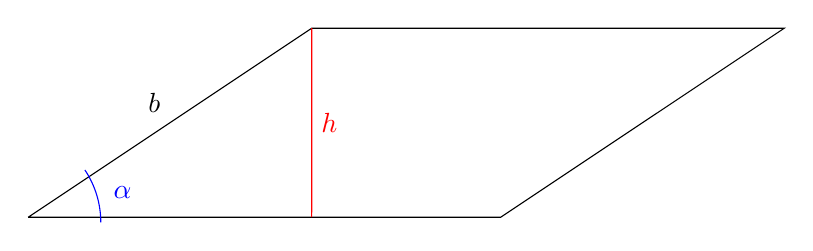
\begin{tikzpicture}[scale=1.2]
    \coordinate (A) at (0,0);
    \coordinate (B) at (5,0);
    \coordinate (C) at (8,2);
    \coordinate (D) at (3,2);
    \draw (A) -- (B) -- (C) -- (D) -- (A);
    \node[red,right] at (3,1) {$h$};
    \draw[red] (3,0) -- (D);
    \node[above left] at (1.5,1) {$\vv{b}$};
    \draw[blue] (0.6,0.5) arc (33.69:0:1);
    \node[blue,above right] at (0.8,0.1) {$\alpha$};
  \end{tikzpicture}
\end{gather*}
\begin{gather*}
  sin(\alpha) = \frac{h}{\vv{b}} \\
  h = |\vv{b}| \cdot sin(\alpha) \\
  A_P = |\vv{a}| \cdot h = |\vv{a}| \cdot |\vv{b}| \cdot sin(\alpha) = |\vv{a} \times \vv{b}|
\end{gather*}
Das Kreuzprodukt $\vv{a} \times \vv{b}$ ergibt einen Vektor als Ergebnis. Die Länge des Vektors $\vv{c}$ ist $|\vv{c}|$ und entspricht dem Flächeninhalt $A_P$ des von den Vektoren $\vv{a}$ und $\vv{b}$ aufgespannten Parallelogramms.
\begin{exercise}{373/1}
  \item [a]
  \begin{gather*}
    \vv{a} = \begin{pmatrix}2 \\ 1 \\ 5\end{pmatrix} \qquad \vv{b} = \begin{pmatrix}3 \\ 2 \\ 1\end{pmatrix} \qquad \vv{c} = \begin{pmatrix}-1 \\ 5 \\ 0\end{pmatrix} \\\\
    \vv{a} \times \vv{b} = \begin{pmatrix}1 \cdot 1 - 5 \cdot 2 \\ 5 \cdot 3 - 2 \cdot 1 \\ 2 \cdot 2 - 1 \cdot 3\end{pmatrix} = \begin{pmatrix}-9 \\ 13 \\ 1\end{pmatrix} \\
    \vv{b} \times \vv{c} = \begin{pmatrix}2 \cdot 0 - 1 \cdot 5 \\ 1 \cdot (-1) - 3 \cdot 0 \\ 3 \cdot 5 - 2 \cdot (-1)\end{pmatrix} = \begin{pmatrix}-5 \\ -1 \\ 17\end{pmatrix} \\
    \vv{c} \times \vv{a} = \begin{pmatrix}5 \cdot 5 - 0 \cdot 1 \\ 0 \cdot 2 - (-1) \cdot 5 \\ -1 \cdot 1 - 5 \cdot 2\end{pmatrix} = \begin{pmatrix}25 \\ 5 \\ -11\end{pmatrix}
  \end{gather*}
\end{exercise}
\newpage
\begin{gather*}
  \vv{a} \times \vv{b} = \vv{c} \qquad \vv{b} \times \vv{a} = -\vv{c}
\end{gather*}
$\vv{a}$, $\vv{b}$, $\vv{c}$ bilden ein Rechtssystem (rechte Hand)
\begin{figure}[H]
  \centering
  \includegraphics[width=0.3\textwidth]{/fakepath/kreuzprodukt.png}
\end{figure}
\begin{exercise}{373/3}
  \item [a]
  \begin{gather*}
    \vv{a} = \begin{pmatrix}3 \\ 2 \\ -1\end{pmatrix} \qquad \vv{b} = \begin{pmatrix}1 \\ 1 \\ 0\end{pmatrix} \\
    \vv{a} \times \vv{b} = \begin{pmatrix}2 \cdot 0 - (-1) \cdot 1 \\ -1 \cdot 1 - 3 \cdot 0 \\ 3 \cdot 1 - 2 \cdot 1\end{pmatrix} = \begin{pmatrix}1 \\ -1 \\ 1\end{pmatrix} \\
    \left|\begin{pmatrix}1 \\ -1 \\ 1\end{pmatrix}\right| = \sqrt{1^2 + (-1)^2 + 1^2} = \sqrt{3} \\
    A_P = \sqrt{3}FE \approx 1.732FE
  \end{gather*}
  \item [b]
  \begin{gather*}
    \vv{a} = \begin{pmatrix}5 \\ -2 \\ 2\end{pmatrix} \qquad \vv{b} = \begin{pmatrix}8 \\ 9 \\ -2\end{pmatrix} \\
    \vv{a} \times \vv{b} = \begin{pmatrix}-2 \cdot (-2) - 2 \cdot 9 \\ 2 \cdot 8 - 5 \cdot (-2) \\ 5 \cdot 9 - (-2) \cdot 8\end{pmatrix} = \begin{pmatrix}-14 \\ 26 \\ 61\end{pmatrix} \\
    \left|\begin{pmatrix}-14 \\ 26 \\ 61\end{pmatrix}\right| = \sqrt{(-14)^2 + 26^2 + 61^2} = \sqrt{4593} \\
    A_P = \sqrt{4593}FE \approx 67.772FE
  \end{gather*}
\end{exercise}
Wenn $\vv{a} \parallel \vv{b}$, also kollinear, dann gilt $\vv{a} \times \vv{b} = \vv{0}$ \\
$|\vv{a} \times \vv{b}| = |\vv{a}| \cdot |\vv{b}| \cdot sin(\alpha)$
\section{Spatprodukt}
\begin{gather*}
  V_{Spat} = G \cdot h = |\vv{a} \times \vv{b}| \cdot h \\
  \;= |\vv{a} \times \vv{b}| \cdot |\vv{c}| \cdot cos(\alpha) \\
  \;= |(\vv{a} \times \vv{b}) \cdot \vv{c}| \qquad \text{(Spatprodukt)}
\end{gather*}
Anwendung: Berechne das Volumen von Spat und Pyramiden
\begin{gather*}
  V_{Spat} = |(\vv{a} \times \vv{b}) \cdot \vv{c}| \\
  V_{Pyramide} = \frac{1}{3} \cdot |(\vv{a} \times \vv{b}) \cdot \vv{c}| \qquad \text{(Grundseite: Parallelogramm des Spats)} \\
  V_{Pyramide,dreiseitig} = \frac{1}{6} \cdot |(\vv{a} \times \vv{b}) \cdot \vv{c}|
\end{gather*}
\begin{exercise}{374/6}
  \item [a]
  \begin{gather*}
    \vv{a} = \begin{pmatrix}-1 \\ 5 \\ 6\end{pmatrix} \qquad \vv{b} = \begin{pmatrix}8 \\ 2 \\ 1\end{pmatrix} \qquad \vv{c} = \begin{pmatrix}-2 \\ 0 \\ 5\end{pmatrix} \\
    V_S = \left|\begin{pmatrix}-1 \\ 5 \\ 6\end{pmatrix} \times \begin{pmatrix}8 \\ 2 \\ 1\end{pmatrix} \cdot \begin{pmatrix}-2 \\ 0 \\ 5\end{pmatrix}\right| = \left|\begin{pmatrix}-7 \\ 49 \\ -42\end{pmatrix} \cdot \begin{pmatrix}-2 \\ 0 \\ 5\end{pmatrix}\right| = 196 \\
    V_P = \frac{1}{6} \cdot 196 = 32.\overline{6}
  \end{gather*}
  \item [b]
  \begin{gather*}
    \vv{a} = \begin{pmatrix}1 \\ 7 \\ 1\end{pmatrix} \qquad \vv{b} = \begin{pmatrix}-8 \\ 8 \\ 18\end{pmatrix} \qquad \vv{c} = \begin{pmatrix}7 \\ 2 \\ 2\end{pmatrix} \\
    V_S = \left|\begin{pmatrix}1 \\ 7 \\ 1\end{pmatrix} \times \begin{pmatrix}-8 \\ 8 \\ 18\end{pmatrix} \cdot \begin{pmatrix}7 \\ 2 \\ 2\end{pmatrix}\right| = \left|\begin{pmatrix}118 \\ -26 \\ 64\end{pmatrix} \cdot \begin{pmatrix}7 \\ 2 \\ 2\end{pmatrix}\right| = 902 \\
    V_P = \frac{1}{6} \cdot 902 = 150.\overline{3}
  \end{gather*}
\end{exercise}
\section{Abstand eines Punktes von einer Geraden}
gegeben:
\begin{gather*}
  g \colon \vv{x} = \vv{a} + r \cdot \vv{b} \\
  P: \vv{p}
\end{gather*}
\begin{gather*}
  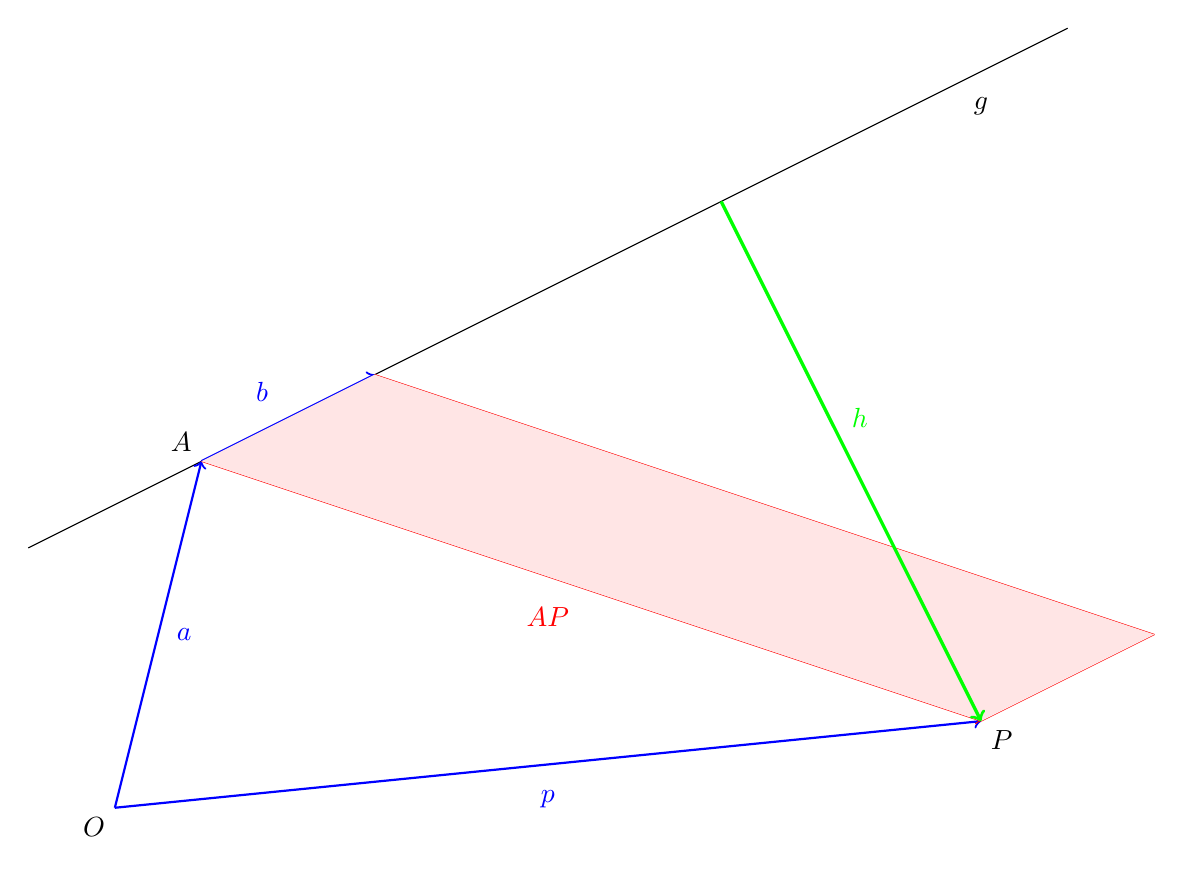
\begin{tikzpicture}[scale=1.1]
    \coordinate (O) at (0,0);
    \coordinate (A) at (1,4);
    \coordinate (B) at (3,5);
    \coordinate (P) at (10,1);
    \coordinate (Q) at (12,2);
    \draw (-1,3) -- (11,9);
    \draw[->,blue,thick] (O) -- (A);
    \draw[->,blue,thick] (O) -- (P);
    \draw[->,blue,thick] (A) -- (B);
    \draw[->,red] (A) -- (P);
    \draw[red] (B) -- (Q);
    \draw[red] (P) -- (Q);
    \fill[red!10] (A) -- (B) -- (Q) -- (P) -- cycle;
    \draw[->,green,very thick] (7,7) -- (P);
    \node[below left] at (O) {$O$};
    \node[above left] at (A) {$A$};
    \node[below right] at (P) {$P$};
    \node at (10,8.1) {$g$};
    \node[blue] at (0.8,2) {$\vv{a}$};
    \node[blue] at (1.7,4.8) {$\vv{b}$};
    \node[blue] at (5,0.1) {$\vv{p}$};
    \node[green] at (8.6,4.5) {$\vv{h}$};
    \node[red] at (5,2.2) {$\vv{AP}$};
  \end{tikzpicture}
\end{gather*}
\begin{gather*}
  \text{Bilde } |\vv{b} \times \vv{AP}| = A_{Parallelogramm} \\
  |\vv{b}| \cdot |\vv{h}| = A_{Parallelogramm} \\\\
  |\vv{b} \times \vv{AP}| = |\vv{b}| \cdot |\vv{h}| \\
  \;\Rightarrow\quad \frac{|\vv{b} \times \vv{AP}|}{|\vv{b}|} = |\vv{h}|
\end{gather*}
$|\vv{h}|$ ist der gesuchte Abstand von Punkt $P$ zur Geraden $g$.
\begin{exercise}{373/5}
  \item [c]
  \begin{gather*}
    g \colon \vv{x} = \begin{pmatrix}1 \\ 1 \\ 0\end{pmatrix} + t \cdot \begin{pmatrix}2 \\ 1 \\ -1\end{pmatrix} \qquad R(-2|-1|1) \\
    \vv{PR} = \begin{pmatrix}-3 \\ -2 \\ 1\end{pmatrix} \qquad \vv{u} = \begin{pmatrix}2 \\ 1 \\ -1\end{pmatrix} \\
    |\vv{h}| = \frac{|\vv{u} \times \vv{PR}|}{|\vv{u}|} = \frac{\left|\begin{pmatrix}-1 \\ 1 \\ -1\end{pmatrix}\right|}{\left|\begin{pmatrix}2 \\ 1 \\ -1\end{pmatrix}\right|} = \frac{\sqrt{3}}{\sqrt{6}} = \sqrt{\frac{1}{2}} \approx 0.7071
  \end{gather*}
  \begin{gather*}
    g \colon \vv{x} = \begin{pmatrix}2 \\ 3 \\ 2\end{pmatrix} + t \cdot \begin{pmatrix}2 \\ -3 \\ -6\end{pmatrix} \qquad R(1|2|-3) \\
    \vv{PR} = \begin{pmatrix}-1 \\ -1 \\ -5\end{pmatrix} \qquad \vv{u} = \begin{pmatrix}2 \\ -3 \\ -6\end{pmatrix} \\
    |\vv{h}| = \frac{|\vv{u} \times \vv{PR}|}{|\vv{u}|} = \frac{\left|\begin{pmatrix}-9 \\ -16 \\ -5\end{pmatrix}\right|}{\left|\begin{pmatrix}2 \\ -3 \\ -6\end{pmatrix}\right|} = \frac{\sqrt{362}}{\sqrt{49}} \approx 2.7180
  \end{gather*}
\end{exercise}
\section{Ebenendarstellung}
\subsection{Normalenform}
\begin{gather*}
  E \colon \vv{x} = \vv{a} + r \cdot \vv{b} + s \cdot \vv{c} \\\\
  E \colon (\vv{x} - \vv{a}) \cdot \vv{n} = 0 \\
  \; \vv{AX} \cdot \vv{n} = 0
\end{gather*}
$\vv{n}$ ... Normalenvektor der Ebene \\
$\vv{a}$ ... Stützvektor, Ortsvektor eines bestimmten Punktes \\
$\vv{x}$ ... allgemeiner Ortsvektor aller Punkte der Ebene \\
$\vv{AX}$ ... Verbindungsvektor, der in der Ebene liegt \\\\
Punkte $X$ der Ebene sind diejenigen, deren Verbindungsvektoren $\vv{AX}$ orthogonal zu $\vv{h}$ stehen. \\\\
z. B.
\begin{gather*}
  \left(\vv{x} - \begin{pmatrix}1 \\ 2 \\ 3\end{pmatrix}\right) \cdot \begin{pmatrix}-1 \\ 0 \\ 4\end{pmatrix} = 0 \\\\
  \text{Beispiellösung } x_1 = \begin{pmatrix}5 \\ 0 \\ 4\end{pmatrix} \\\\
  \text{Punktprobe } P(2|1|1) \quad P \in E ? \\
  \begin{pmatrix}2 - 1 \\ 1 - 2 \\ 1 - 3\end{pmatrix} \cdot \begin{pmatrix}-1 \\ 0 \\ 4\end{pmatrix} = 0 \qquad -1 + 0 - 8 = -9 \neq 0 \quad\Rightarrow\quad P \not\in E
\end{gather*}
Normalengleichung aus $A(1|0|5)$, $B(0|2|1)$, $C(4|5|6)$
\begin{gather*}
  E \colon \vv{x} = \begin{pmatrix}1 \\ 0 \\ 5\end{pmatrix} + r \cdot \begin{pmatrix}-1 \\ 2 \\ -4\end{pmatrix} + s \cdot \begin{pmatrix}3 \\ 5 \\ 1\end{pmatrix} \\
  \vv{n} = \vv{AB} \times \vv{AC} = \begin{pmatrix}-1 \\ 2 \\ -4\end{pmatrix} \times \begin{pmatrix}3 \\ 5 \\ 1\end{pmatrix} = \begin{pmatrix}22 \\ -11 \\ -11\end{pmatrix} \\
  E \colon \left(\vv{x} - \begin{pmatrix}1 \\ 0 \\ 5\end{pmatrix}  \right) \cdot \begin{pmatrix}22 \\ -11 \\ -11\end{pmatrix} = 0
\end{gather*}
\subsection{Koordinatenform}
Berechne das Skalarprodukt in der Normalengleichung mit $\vv{x} = \begin{pmatrix}x_1 \\ x_2 \\ x_3\end{pmatrix}$
\begin{gather*}
  E \colon \left(\begin{pmatrix}x_1 \\ x_2 \\ x_3\end{pmatrix} - \begin{pmatrix}a_1 \\ a_2 \\ a_3\end{pmatrix}\right) \cdot \begin{pmatrix}n_1 \\ n_2 \\ n_3\end{pmatrix} = 0 \\
  \begin{pmatrix}x_1 \\ x_2 \\ x_3\end{pmatrix} \cdot \begin{pmatrix}n_1 \\ n_2 \\ n_3\end{pmatrix} - \begin{pmatrix}a_1 \\ a_2 \\ a_3\end{pmatrix} \cdot \begin{pmatrix}n_1 \\ n_2 \\ n_3\end{pmatrix} = 0 \\
  (n_1 \cdot x_1 + n_2 \cdot x_2 + n_3 \cdot x_3) - (a_1 \cdot n_1 + a_2 \cdot n_2 + a_3 \cdot n_3) = 0 \\\\
  \text{z. B. } 22x_1 - 11x_2 - 11x_3 = -33 \\
  \text{Beispiellösungen } \vv{x} = \begin{pmatrix}-1 \\ 1 \\ 0\end{pmatrix}, \begin{pmatrix}1 \\ 2 \\ 3\end{pmatrix}, \begin{pmatrix}2 \\ 1 \\ 6\end{pmatrix}, ...
\end{gather*}
\begin{gather*}
  E \colon ax_1 + bx_2 + cx_3 = d
\end{gather*}
Betrache die Koordinatenform als eine Gleichung für drei Variablen $x_1$, $x_2$, $x_3$. Die Lösungen der Gleichung sind Dreiertupel $L = \{(...,\;...,\;...),\;...\}$. Notiere ich die Dreiertupel als Spaltenvektoren, so stellen sie die Ortsvektoren der Punkte der Ebene $E$ dar. Die Koeffizienten $a$, $b$, $c$ der Koordinatenform sind die Koordinaten von $\vv{n}$, des Normalenvektors.
\subsubsection{Koordinatenform $\rightarrow$ Normalenform}
\begin{gather*}
  \text{z. B. } 5x_1 - x_2 + 3x_3 = 9
\end{gather*}
\begin{enumerate}
  \item Lies ab $\vv{n} = \begin{pmatrix}5 \\ -1 \\ 3\end{pmatrix}$
  \item Finde eine Lösung $\begin{pmatrix}x_1 \\ x_2 \\ x_3\end{pmatrix}$, z. B. $\begin{pmatrix}0 \\ 0 \\ 3\end{pmatrix}$
\end{enumerate}
\begin{gather*}
  E \colon \left(\vv{x} - \begin{pmatrix}0 \\ 0 \\ 3\end{pmatrix}\right) \cdot \begin{pmatrix}5 \\ -1 \\ 3\end{pmatrix} = 0
\end{gather*}
\subsubsection{Sonderfälle}
\begin{itemize}
  \item
  \begin{gather*}
    E \colon x_3 = 5 \quad\rightarrow\quad \vv{n} = \begin{pmatrix}0 \\ 0 \\ 1\end{pmatrix}
  \end{gather*}
  Punkte der Ebene haben $x_3 = 5$; $x_1$, $x_2$ sind beliebige Koordinaten.
  \begin{gather*}
    \text{z. B. } \begin{pmatrix}1 \\ 1 \\ 5\end{pmatrix}, \begin{pmatrix}-2 \\ 3 \\ 5\end{pmatrix}, \begin{pmatrix}0 \\ 7 \\ 5\end{pmatrix}, ...
  \end{gather*}
  $x_1$ und $x_2$ sind nicht erwähnt, also frei wählbar.
  \item
  \begin{gather*}
    E \colon 2x_1 - 4x_2 = 0
  \end{gather*}
  Der Ursprung $O$ ist Teil der Ebene $E$. Der Verbindungsvektor $\vv{O} - \vv{a}$, also der Ortsvektor $\vv{a}$ liegt in der Ebene $E$ und steht orthogonal zu $\vv{n}$. Daher sind $\vv{a} \cdot \vv{n} = 0$ und damit $d = 0$.
\end{itemize}
\begin{exercise}{325/3}
  \begin{gather*}
    D(-7|1|3)
  \end{gather*}
  \item [a]
  \begin{gather*}
    A(1|1|1) \qquad B(1|0|1) \qquad C(0|1|1) \\
    \vv{AB} = \begin{pmatrix}0 \\ -1 \\ 0\end{pmatrix} \qquad \vv{AC} = \begin{pmatrix}-1 \\ 0 \\ 0\end{pmatrix} \\
    \vv{n} = \vv{AB} \times \vv{AC} = \begin{pmatrix}0 \\ 0 \\ -1\end{pmatrix} \\\\
    E \colon \left(\vv{x} - \begin{pmatrix}1 \\ 1 \\ 1\end{pmatrix}\right) \cdot \begin{pmatrix}0 \\ 0 \\ -1\end{pmatrix} = 0 \\
    E \colon -x_3 = 0 + 0 - 1 = -1 \\\\
    D \in E ? \qquad -x_3 = -3 \neq -1 \qquad \Rightarrow\quad D \not\in E
  \end{gather*}
  \item [b]
  \begin{gather*}
    A(-1|2|0) \qquad B(-3|1|1) \qquad C(1|-1|-1) \\
    \vv{AB} = \begin{pmatrix}-2 \\ -1 \\ 1\end{pmatrix} \qquad \vv{AC} = \begin{pmatrix}2 \\ -3 \\ -1\end{pmatrix} \\
    \vv{n} = \vv{AB} \times \vv{AC} = \begin{pmatrix}4 \\ 0 \\ 8\end{pmatrix} \\\\
    E \colon \left(\vv{x} - \begin{pmatrix}-1 \\ 2 \\ 0\end{pmatrix}\right) \cdot \begin{pmatrix}4 \\ 0 \\ 8\end{pmatrix} = 0 \\
    E \colon 4x_1 + 8x_3 = -4 + 0 + 0 = -4 \\\\
    D \in E? \qquad 4x_1 + 8x_3 = -28 + 24 = -4 \qquad \Rightarrow\quad D \in E
  \end{gather*}
\end{exercise}
\subsection{Ebenen zeichnen}
Zeichne Ebene $E \colon 2x_1 - 3x_2 + 5x_3 = 12$ \\\\
Schnitt mit der ...
\begin{itemize}
  \item [] $x_1$-Achse:
  \begin{gather*}
    x_2 = x_3 = 0 \quad\Rightarrow\quad 2x_1 = 12 \quad x_1 = 6 \quad P(6|0|0)
  \end{gather*}
  \item [] $x_2$-Achse:
  \begin{gather*}
    x_1 = x_3 = 0 \quad\Rightarrow\quad -3x_2 = 12 \quad x_2 = -4 \quad Q(0|-4|0)
  \end{gather*}
  \item [] $x_3$-Achse:
  \begin{gather*}
    x_1 = x_2 = 0 \quad\Rightarrow\quad 5x_3 = 12 \quad x_3 = 2.4 \quad R(0|0|2.4)
  \end{gather*}
\end{itemize}
$P$, $Q$, $R$ heißen Spurpunkte. \\
Gerade durch $P$ und $Q$ (bzw. $Q$ und $R$, $P$ und $R$) heißt Spurgerade.
\begin{gather*}
  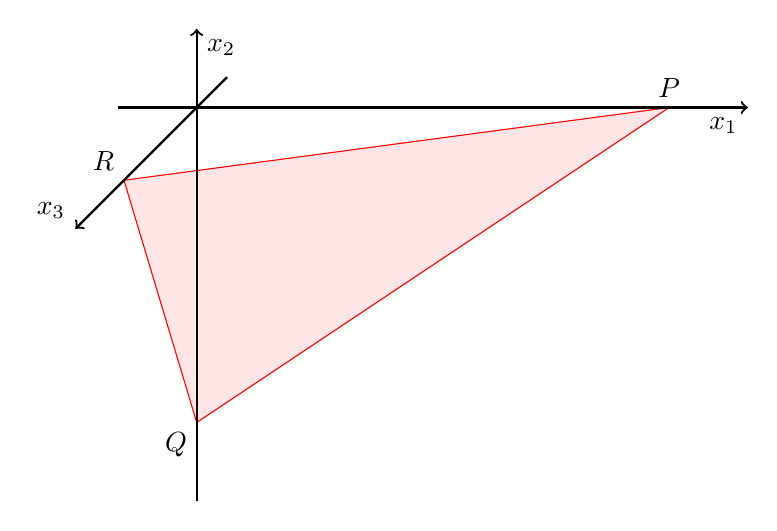
\begin{tikzpicture}
    \coordinate (P) at (6,0,0);
    \coordinate (Q) at (0,-4,0);
    \coordinate (R) at (0,0,2.4);
    \node[above] at (P) {$P$};
    \node[below left] at (Q) {$Q$};
    \node[above left] at (R) {$R$};
    \draw[red,fill=red!10] (P) -- (Q) -- (R) -- (P);
    \draw[thick,->] (-1,0,0) -- (7,0,0) node[anchor=north east]{$x_1$};
    \draw[thick,->] (0,-5,0) -- (0,1,0) node[anchor=north west]{$x_2$};
    \draw[thick,->] (0,0,-1) -- (0,0,4) node[anchor=south east]{$x_3$};
  \end{tikzpicture}
\end{gather*}
Spurgerade (PQ):
\begin{gather*}
  g \colon \vv{x} = \begin{pmatrix}0 \\ -4 \\ 0\end{pmatrix} + r \cdot \begin{pmatrix}6 \\ 4 \\ 0\end{pmatrix}
\end{gather*}
Spezialfälle
\begin{itemize}
  \item
  \begin{gather*}
    3x_1 + 6x_3 = 18 \qquad P(6|0|0) \quad R(0|0|3) \quad Q(0|\infty|0)
  \end{gather*}
  Kein Schnitt mit der $x_2$-Achse, verläuft parallel zur $x_2$-Achse.
  \item
  \begin{gather*}
    2x_1 = 5 \qquad P(2.5|0|0)
  \end{gather*}
  Kein Schnitt mit der $x_2$- und $x_3$-Achse, verläuft parallel zur $x_2x_3$-Ebene.
\end{itemize}
\begin{exercise}{328/3}
  Fig. 1
  \begin{gather*}
    P(2|0|0) \qquad Q(0|5|0) \qquad R(0|0|3) \\
    15x_1 = 30 \qquad 6x_2 = 30 \qquad 10x_3 = 30 \\
    E \colon 15x_1 + 6x_2 + 10x_3 = 30
  \end{gather*}
  Fig. 2
  \begin{gather*}
    P(1|0|0) \qquad Q(0|4|0) \qquad R(0|0|-1.5) \\
    12x_1 = 12 \qquad 3x_2 = 12 \qquad -8x_3 = 12 \\
    E \colon 12x_1 + 3x_2 - 8x_3 = 12
  \end{gather*}
\end{exercise}
\begin{exercise}{328/5}
  \item [a]
  \begin{gather*}
    E \colon \vv{x} = \begin{pmatrix}1 \\ 2 \\ 3\end{pmatrix} + r \cdot \begin{pmatrix}-1 \\ 2 \\ 0\end{pmatrix} + s \cdot \begin{pmatrix}1 \\ 0 \\ 3\end{pmatrix} \\
    \vv{n} = \begin{pmatrix}-1 \\ 2 \\ 0\end{pmatrix} \times \begin{pmatrix}1 \\ 0 \\ 3\end{pmatrix} = \begin{pmatrix}6 \\ 3 \\ -2\end{pmatrix} \qquad \begin{pmatrix}1 \\ 2 \\ 3\end{pmatrix} \cdot \vv{n} = 6 \\
    E \colon 6x_1 + 3x_2 - 2x_3 = 6 \\
    P(1|0|0) \qquad Q(0|2|0) \qquad R(0|0|-3)
  \end{gather*}
  \begin{gather*}
    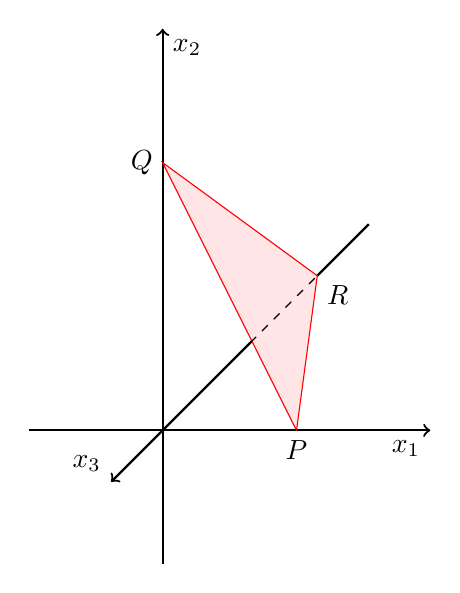
\begin{tikzpicture}[scale=1.7]
      \coordinate (P) at (1,0,0);
      \coordinate (Q) at (0,2,0);
      \coordinate (R) at (0,0,-3);
      \node[below] at (P) {$P$};
      \node[left] at (Q) {$Q$};
      \node[below right] at (R) {$R$};
      \draw[thick,->] (-1,0,0) -- (2,0,0) node[anchor=north east]{$x_1$};
      \draw[thick,->] (0,-1,0) -- (0,3,0) node[anchor=north west]{$x_2$};
      \draw[thick,->] (0,0,-4) -- (0,0,1) node[anchor=south east]{$x_3$};
      \draw[red,fill=red!10] (P) -- (Q) -- (R) -- (P);
      \draw[dashed] (0,0,-1.7) -- (R);
    \end{tikzpicture}
  \end{gather*}
  \item [b]
  \begin{gather*}
    E \colon \vv{x} = \begin{pmatrix}1 \\ 1 \\ 1\end{pmatrix} + r \cdot \begin{pmatrix}5 \\ 0 \\ 5\end{pmatrix} + s \cdot \begin{pmatrix}0 \\ 1 \\ 4\end{pmatrix} \\
    \vv{n} = \begin{pmatrix}5 \\ 0 \\ 5\end{pmatrix} \times \begin{pmatrix}0 \\ 1 \\ 4\end{pmatrix} = \begin{pmatrix}-5 \\ -20 \\ 5\end{pmatrix} \qquad \begin{pmatrix}1 \\ 1 \\ 1\end{pmatrix} \cdot \vv{n} = -20 \\
    E \colon -5x_1 - 20x_2 + 5x_3 = -20 \\
    P(4|0|0) \qquad Q(0|1|0) \qquad R(0|0|-4)
  \end{gather*}
  \begin{gather*}
    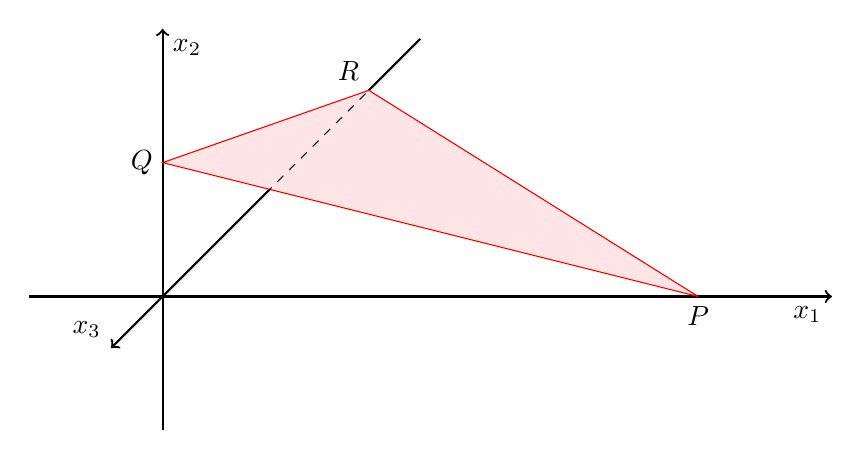
\begin{tikzpicture}[scale=1.7]
      \coordinate (P) at (4,0,0);
      \coordinate (Q) at (0,1,0);
      \coordinate (R) at (0,0,-4);
      \node[below] at (P) {$P$};
      \node[left] at (Q) {$Q$};
      \node[above left] at (R) {$R$};
      \draw[thick,->] (-1,0,0) -- (5,0,0) node[anchor=north east]{$x_1$};
      \draw[thick,->] (0,-1,0) -- (0,2,0) node[anchor=north west]{$x_2$};
      \draw[thick,->] (0,0,-5) -- (0,0,1) node[anchor=south east]{$x_3$};
      \draw[red,fill=red!10] (P) -- (Q) -- (R) -- (P);
      \draw[dashed] (0,0,-2) -- (R);
    \end{tikzpicture}
  \end{gather*}
\end{exercise}
\begin{exercise}{328/6}
  Fig. 3
  \begin{gather*}
    P(0|3|0) \\
    E \colon x_2 = 3 \\
    \text{parallel zur $x_1x_3$-Ebene}
  \end{gather*}
  Fig. 4
  \begin{gather*}
    P(1|0|0) \qquad Q(0|5|0) \\
    5x_1 = 5 \qquad x_2 = 5 \\
    E \colon 5x_1 + x_2 = 5 \\
    \text{parallel zur $x_3$-Ebene}
  \end{gather*}
\end{exercise}
\section{Lage Ebene $\leftrightarrow$ Gerade}
\begin{itemize}
  \item schneiden sich
  \item verlaufen parallel
  \item Gerade ist Teil der Ebene
\end{itemize}
Beispiel:
\begin{gather*}
  E \colon 2x_1 - x_2 + 3x_3 = 16 \\
  g \colon \vv{x} = \begin{pmatrix}1 \\ 2 \\ 3\end{pmatrix} + r \cdot \begin{pmatrix}2 \\ -1 \\ 0\end{pmatrix} = \begin{pmatrix}1 + 2r \\ 2 - r \\ 3\end{pmatrix} = \begin{pmatrix}x_1 \\ x_2 \\ x_3\end{pmatrix} \\\\
  \text{$g$ in $E$ eingesetzt} \\
  2 \cdot (1 + 2r) - (2 - r) + 3 \cdot 3 = 16 \\
  \Rightarrow\quad r = \frac{7}{5} \\
  \text{Schnittpunkt } \vv{OS} = \begin{pmatrix}1 \\ 2 \\ 3\end{pmatrix} + \frac{7}{5} \cdot \begin{pmatrix}2 \\ -1 \\ 0\end{pmatrix} = \begin{pmatrix}3.8 \\ 0.6 \\ 3\end{pmatrix}
\end{gather*}
\begin{itemize}
  \item eindeutige Lösung für $r$ $\Rightarrow$ schneiden sich
  \item kein $r$ erfüllt die Gleichung $\Rightarrow$ kein Schnittpunkt, parallele Lage
  \item für jedes $r$ ein möglicher gemeinsamer Punkt $\Rightarrow$ Gerade liegt in der Ebene
\end{itemize}
\begin{exercise}{330/1}
  \begin{gather*}
    g \colon \vv{x} = \begin{pmatrix}4 \\ 6 \\ 2\end{pmatrix} + t \cdot \begin{pmatrix}1 \\ 2 \\ 3\end{pmatrix}
  \end{gather*}
  \item [a]
  \begin{gather*}
    E \colon 2x_1 + 4x_2 + 6x_3 = 16 \\\\
    2 \cdot (4 + t) + 4 \cdot (6 + 2t) + 6 \cdot (2 + 3t) = 16 \\
    \Rightarrow\quad t = -1 \\\\
    \begin{pmatrix}4 \\ 6 \\ 2\end{pmatrix} - 1 \cdot \begin{pmatrix}1 \\ 2 \\ 3\end{pmatrix} = \begin{pmatrix}3 \\ 4 \\ -1\end{pmatrix} \\\\
    S(3|4|-1)
  \end{gather*}
  \item [b]
  \begin{gather*}
    E \colon 5x_2 - 7x_3 = 13 \\\\
    5 \cdot (6 + 2t) - 7 \cdot (2 + 3t) = 13 \\
    t = \frac{3}{11} \\\\
    \begin{pmatrix}4 \\ 6 \\ 2\end{pmatrix} + \frac{3}{11} \cdot \begin{pmatrix}1 \\ 2 \\ 3\end{pmatrix} = \begin{pmatrix}4.\overline{27} \\ 6.\overline{54} \\ 2.\overline{81}\end{pmatrix} \\\\
    S(4.\overline{27}|6.\overline{54}|2.\overline{81})
  \end{gather*}
\end{exercise}
\begin{exercise}{330/2}
  \item [a]
  \begin{gather*}
    g \colon \vv{x} = \begin{pmatrix}-2 \\ 1 \\ 4\end{pmatrix} + t \cdot \begin{pmatrix}7 \\ 8 \\ 6\end{pmatrix} \qquad E \colon \vv{x} = \begin{pmatrix}1 \\ 4 \\ 3\end{pmatrix} + r \cdot \begin{pmatrix}0 \\ -1 \\ 1\end{pmatrix} + s \cdot \begin{pmatrix}1 \\ 0 \\ 3\end{pmatrix} \\\\
    -2 + 7t = 1 + s \\
    1 + 8t = 4 - r \\
    4 + 6t = 3 + r + 3s \\
    t = 1 \qquad r = -5 \qquad s = 4 \\\\
    \begin{pmatrix}-2 \\ 1 \\ 4\end{pmatrix} + 1 \cdot \begin{pmatrix}7 \\ 8 \\ 6\end{pmatrix} = \begin{pmatrix}5 \\ 9 \\ 10\end{pmatrix} \\\\
    S(5|9|10)
  \end{gather*}
  \item [b]
  \begin{gather*}
    g \colon \vv{x} = \begin{pmatrix}22 \\ -18 \\ -7\end{pmatrix} + t \cdot \begin{pmatrix}4 \\ 1 \\ -5\end{pmatrix} \qquad E \colon \vv{x} = \begin{pmatrix}2 \\ 1 \\ 0\end{pmatrix} + r \cdot \begin{pmatrix}4 \\ -7 \\ 1\end{pmatrix} + s \cdot \begin{pmatrix}0 \\ 4 \\ -3\end{pmatrix} \\\\
    22 + 4t = 2 + 4r \\
    -18 + t = 1 - 7r + 4s \\
    -7 - 5t = r - 3s \\\\
    t = r - 5 \qquad s = 2r - 6 \\\\
    g \in E
  \end{gather*}
  \item [c]
  \begin{gather*}
    g \colon \vv{x} = t \cdot \begin{pmatrix}-1 \\ -1 \\ -1\end{pmatrix} \qquad E \colon \vv{x} = \begin{pmatrix}0 \\ 0 \\ 2\end{pmatrix} + r \cdot \begin{pmatrix}2 \\ 0 \\ 0\end{pmatrix} + s \cdot \begin{pmatrix}0 \\ 2 \\ 0\end{pmatrix} \\\\
    -t = 2r \\
    -t = 2s \\
    -t = 2 \\\\
    t = -2 \qquad r = 1 \qquad s = 1 \\\\
    -2 \cdot \begin{pmatrix}-1 \\ -1 \\ -1\end{pmatrix} = \begin{pmatrix}2 \\ 2 \\ 2\end{pmatrix} \\\\
    S(2|2|2)
  \end{gather*}
\end{exercise}
\subsection{Schnittwinkel}
\begin{gather*}
  g \colon \vv{x} = \vv{a} + r \cdot \vv{b} \qquad h \colon \vv{x} = \vv{c} + s \cdot \vv{d} \\\\
  \vv{b} \cdot \vv{d} = |\vv{b}| \cdot |\vv{d}| \cdot cos(\alpha) \\
  \alpha = acos\left(\frac{\vv{b} \cdot \vv{d}}{|\vv{b}| \cdot |\vv{d}|}\right) \qquad \alpha < 90^\circ \\\\
  \alpha = acos\left(\frac{\vv{n} \cdot \vv{b}}{|\vv{n}| \cdot |\vv{b}|}\right) \qquad \beta = asin\left(\frac{\vv{n} \cdot \vv{b}}{|\vv{n}| \cdot |\vv{b}|}\right) \qquad \beta = 90^\circ - \alpha
\end{gather*}
\section{Wiederholung}
\begin{exercise}{344/7}
  \begin{gather*}
    g_a \colon \vv{x} = \begin{pmatrix}2 \\ 7 \\ 3\end{pmatrix} + t \cdot \begin{pmatrix}4 + 2a \\ -1 + 5a \\ 1 + 3a\end{pmatrix} \qquad a \in \mathbb{R} \\
    P(1|0|2),\; Q(2|0|3),\; R(0|2|2) \in E
  \end{gather*}
  \item [a]
  \begin{gather*}
    \vv{PQ} = \begin{pmatrix}1 \\ 0 \\ 1\end{pmatrix} \qquad \vv{PR} = \begin{pmatrix}-1 \\ 2 \\ 0\end{pmatrix} \\
    \vv{n} = \vv{PQ} \times \vv{PR} = \begin{pmatrix}-2 \\ -1 \\ 2\end{pmatrix} \qquad \vv{OP} \cdot \vv{n} = 2 \\
    E \colon -2x_1 - x_2 + 2x_3 = 2 \\\\
    g_0 \colon \vv{x} = \begin{pmatrix}2 \\ 7 \\ 3\end{pmatrix} + t \cdot \begin{pmatrix}4 \\ -1 \\ 1\end{pmatrix} \qquad g_1 \colon \vv{x} = \begin{pmatrix}2 \\ 7 \\ 3\end{pmatrix} + t \cdot \begin{pmatrix}6 \\ 4 \\ 4\end{pmatrix} \\\\
    g_0 = E \qquad -2(2 + 4t) - (7 - t) + 2(3 + t) = 2 \quad\Rightarrow\quad t = -\frac{7}{5} \\
    g_1 = E \qquad -2(2 + 6t) - (7 + 4t) + 2(3 + 4t) = 2 \quad\Rightarrow\quad t = \frac{-7}{8} \\\\
  \end{gather*}
  \begin{gather*}
    \vv{OS_0} = \begin{pmatrix}2 \\ 7 \\ 3\end{pmatrix} - \frac{7}{5} \cdot \begin{pmatrix}4 \\ -1 \\ 1\end{pmatrix} = \begin{pmatrix}-3.6 \\ 8.4 \\ 1.6\end{pmatrix} \qquad \vv{OS_1} = \begin{pmatrix}2 \\ 7 \\ 3\end{pmatrix} - \frac{7}{8} \cdot \begin{pmatrix}6 \\ 4 \\ 4\end{pmatrix} = \begin{pmatrix}-3.25 \\ 3.5 \\ -0.5\end{pmatrix} \\
    \vv{S_0S_1} = \begin{pmatrix}0.35 \\ -4.9 \\ -2.1\end{pmatrix} \\\\
    h \colon \vv{x} = \begin{pmatrix}-3.6 \\ 8.4 \\ 1.6\end{pmatrix} + t \cdot \begin{pmatrix}0.35 \\ -4.9 \\ -2.1\end{pmatrix}
  \end{gather*}
  \item [b]
  \begin{gather*}
    t \cdot \begin{pmatrix}0.35 \\ -4.9 \\ -2.1\end{pmatrix} = \begin{pmatrix}4 + 2a \\ -1 + 5a \\ 1 + 3a\end{pmatrix} \\\\
    0.35t = 4 + 2a \\
    -4.9t = -1 + 5a \\
    -2.1t = 1 + 3a \\\\
    \Rightarrow\quad a = -\frac{5}{3} \qquad (t \approx 1.905)
  \end{gather*}
\end{exercise}
\begin{exercise}{326/15}
  \item [a]
  \begin{gather*}
    2t = 0 \quad\Rightarrow\quad t = 0 \\
    4 = 0 \quad\Rightarrow\quad \text{keine Lösung} \\
    t = 0 \quad\Rightarrow\quad t = 0 \\\\
    \Rightarrow\quad t = 0
  \end{gather*}
  \item [b]
  \begin{gather*}
    t - 1 = 0 \quad\Rightarrow\quad t = 1 \\
    t^2 - 1 = 0 \quad\Rightarrow\quad t = \pm1 \\
    t + 1 = 0 \quad\Rightarrow\quad t = -1 \\\\
    \Rightarrow\quad t = \pm1
  \end{gather*}
\end{exercise}
\newpage
\begin{exercise}{374/7}
  \item [b]
  \begin{gather*}
    A(1|-2|12) \qquad B(11|3|5) \qquad C(3|5|8) \qquad D(19|4|4) \\
    \vv{AB} = \begin{pmatrix}10 \\ 5 \\ -7\end{pmatrix} \qquad \vv{AC} = \begin{pmatrix}2 \\ 7 \\ -4\end{pmatrix} \qquad \vv{AD} = \begin{pmatrix}18 \\ 6 \\ -8\end{pmatrix} \\
    V = \frac{1}{6} \cdot |\vv{AB} \times \vv{AC} \cdot \vv{AD}| = \frac{1}{6} \cdot \left|\begin{pmatrix}10 \\ 5 \\ -7\end{pmatrix} \times \begin{pmatrix}2 \\ 7 \\ -4\end{pmatrix} \cdot \begin{pmatrix}18 \\ 6 \\ -8\end{pmatrix}\right| \\
    \;= \frac{1}{6} \cdot \left|\begin{pmatrix}29 \\ 26 \\ 60\end{pmatrix} \cdot \begin{pmatrix}18 \\ 6 \\ -8\end{pmatrix}\right| = \frac{1}{6} \cdot |198| = 33
  \end{gather*}
\end{exercise}
\section{Lage Ebene $\leftrightarrow$ Ebene}
3 Fälle sind möglich:
\begin{itemize}
  \item 2 Ebenen schneiden sich in einer Geraden (Normalenvektoren sind nicht kollinear)
  \begin{gather*}
    2x_1 - x_2 = 7 \qquad \vv{n} = \begin{pmatrix}2 \\ -1 \\ 0\end{pmatrix} \\
    5x_2 + x_3 = 5 \qquad \vv{n} = \begin{pmatrix}0 \\ 5 \\ 1\end{pmatrix}
  \end{gather*}
  \item 2 Ebenen sind parallel (kollineare Normalenvektoren)
  \begin{gather*}
    2x_1 - x_2 = 7 \qquad \vv{n} = \begin{pmatrix}2 \\ -1 \\ 0\end{pmatrix} \\
    10x_1 - 5x_2 = 1 \qquad \vv{n} = \begin{pmatrix}10 \\ -5 \\ 0\end{pmatrix}
  \end{gather*}
  \item 2 Ebenen sind identisch (Koordinatengleichungen lassen sich ineinander umformen)
  \begin{gather*}
    2x_1 - x_2 = 7 \equ \cdot 5 \\
    10x_1 - 5x_2 = 35
  \end{gather*}
\end{itemize}
\begin{gather*}
  E \colon \vv{x} = \begin{pmatrix}1 \\ 2 \\ 3\end{pmatrix} + r \cdot \begin{pmatrix}0 \\ 1 \\ 3\end{pmatrix} + s \cdot \begin{pmatrix}-1 \\ 0 \\ 5\end{pmatrix} = \begin{pmatrix}1 - s \\ 2 + r \\ 3 + 3r + 5s\end{pmatrix} = \begin{pmatrix}x_1 \\ x_2 \\ x_3\end{pmatrix} \\
  F \colon \vv{x} = x_1 - x_2 + 3x_3 = 5 \\\\
  \text{setze $E$ in $F$ ein} \\
  1 - s - (2 + r) + 3 \cdot (3 + 3r + 5s) = 5 \\
  8r + 14s = -3 \\
  r = -\frac{3}{8} - \frac{14}{8}s \\\\
  g \colon \vv{x} = \begin{pmatrix}1 - s \\ 2 - \frac{3}{8} - \frac{14}{8}s \\[0.4em] 3 + 3 \cdot (-\frac{3}{8} - \frac{14}{8}s) + 5s\end{pmatrix} = \begin{pmatrix}1 \\ \frac{13}{8} \\[0.4em] \frac{15}{8}\end{pmatrix} + s \cdot \begin{pmatrix}-1 \\ -\frac{7}{4} \\[0.4em] -\frac{1}{4}\end{pmatrix}
\end{gather*}
\begin{exercise}{333/2}
  \item [a]
  \begin{gather*}
    E_1 \colon x_1 - x_2 + 2x_3 = 7 \qquad E_2 \colon 6x_1 + x_2 - x_3 = -7 \\\\
    x_3 = 3.5 - 0.5x_1 + 0.5x_3 \\
    E_1 \colon \vv{x} = \begin{pmatrix}0 \\ 0 \\ 3.5\end{pmatrix} + r \cdot \begin{pmatrix}1 \\ 0 \\ -0.5\end{pmatrix} + s \cdot \begin{pmatrix}0 \\ 1 \\ 0.5\end{pmatrix} = \begin{pmatrix}r \\ s \\ 3.5 - 0.5r + 0.5s\end{pmatrix} \\\\
    \text{$E_1$ in $E_2$ einsetzen:} \\
    6r + s - (3.5 - 0.5r + 0.5s) = -7 \\
    s = -7 - 13r \\\\
    g \colon \vv{x} = \begin{pmatrix}r \\ -7 - 13r \\ -7r\end{pmatrix} = \begin{pmatrix}0 \\ -7 \\ 0\end{pmatrix} + r \cdot \begin{pmatrix}1 \\ -13 \\ -7\end{pmatrix}
  \end{gather*}
\end{exercise}
\newpage
\begin{exercise}{334/3}
  \item [a]
  \begin{gather*}
    E_1 \colon \vv{x} = \begin{pmatrix}1 \\ 0 \\ 3\end{pmatrix} + r \cdot \begin{pmatrix}1 \\ 0 \\ 0\end{pmatrix} + s \cdot \begin{pmatrix}1 \\ 1 \\ 0\end{pmatrix} \qquad E_2 \colon \vv{x} = \begin{pmatrix}2 \\ 3 \\ 2\end{pmatrix} + r \cdot \begin{pmatrix}0 \\ 1 \\ 1\end{pmatrix} + s \cdot \begin{pmatrix}2 \\ 0 \\ 1\end{pmatrix} \\\\
    E_2 \colon x_1 + 2x_2 - 2x_3 = 4 \\\\
    \text{$E_1$ in $E_2$ einsetzen:} \\
    1 + r + s + 2s - 2 \cdot 3 = 4 \\
    r = 9 - 3s \\\\
    g \colon \vv{x} = \begin{pmatrix}10 - 2s \\ s \\ 3\end{pmatrix} = \begin{pmatrix}10 \\ 0 \\ 3\end{pmatrix} + s \cdot \begin{pmatrix}-2 \\ 1 \\ 0\end{pmatrix}
  \end{gather*}
\end{exercise}
\section{Abstand Ebene $\leftrightarrow$ Punkt}
Fußlotpunkt-Methode
\begin{gather*}
  E \colon \left(\vv{x} - \begin{pmatrix}1 \\ 2 \\ 3\end{pmatrix}\right) \cdot \begin{pmatrix}1 \\ 0 \\ 4\end{pmatrix} = 0 \qquad P(8|-3|0) \\\\
  \text{orthogonale Gerade durch Punkt $P$} \\
  g \colon \vv{x} = \begin{pmatrix}8 \\ -3 \\ 0\end{pmatrix} + r \cdot \begin{pmatrix}1 \\ 0 \\ 4\end{pmatrix} \\\\
  \text{Schnittpunkt $g \leftrightarrow E$} \\
  \text{$g$ in $E$} \quad \begin{pmatrix}8 + r - 1 \\ -3 - 2 \\ 0 + 4r - 3\end{pmatrix} \cdot \begin{pmatrix}1 \\ 0 \\ 4\end{pmatrix} = 0 \\
  \vv{OS} = \begin{pmatrix}\frac{141}{17} \\ -3 \\ \frac{20}{17}\end{pmatrix} \qquad r = \frac{5}{17} \\\\
  \text{Abstand $P \leftrightarrow E$ ist $|\vv{PS}|$} \\
  d(P, E) = 1.21LE
\end{gather*} \\
Hessesche Normalenform (HNF)
\begin{gather*}
  E_0 \colon \left(\vv{x} - \begin{pmatrix}1 \\ 2 \\ 3\end{pmatrix}\right) \cdot \underbrace{\frac{1}{\sqrt{17}} \cdot \begin{pmatrix}1 \\ 0 \\ 4\end{pmatrix}}_{\mathclap{\text{Normaleneinheitsvektor $\vv{n_0} \quad |\vv{n_0}| = 1$}}} = 0 \\\\
  \text{setze $P$ für $\vv{x}$ in $E_0$ ein} \\
  \left|\left(\begin{pmatrix}8 \\ -3 \\ 0\end{pmatrix} - \begin{pmatrix}1 \\ 2 \\ 3\end{pmatrix}\right) \cdot \frac{1}{\sqrt{17}} \cdot \begin{pmatrix}1 \\ 0 \\ 4\end{pmatrix}\right| = d \\\\
  d(P, E) = 1.21LE
\end{gather*}
\begin{gather*}
  \begin{tikzpicture}[scale=2]
    \coordinate[label=below:$A$] (A) at (0,0);
    \coordinate[label=below:$S$] (S) at (-3,0);
    \coordinate[label=above left:$P$] (P) at (-3,3);
    \draw[ultra thick] (-5,0) -- (2,0);
    \node[above right] at (-5,0) {$E$};
    \draw (A) -- (P);
    \draw[color=red] (P) -- (S);
    \draw[arrows={-triangle 45}] (A) -- (0,1);
    \node[below right] at (0,1) {$\vv{n_0}$};
    \draw[arrows={-triangle 45}] (A) -- (0,3);
    \node[below right] at (0,3) {$\vv{AP}_{\vv{n}}$};
    \draw[dashed,lightgray] (P) -- (0,3);
    \draw[arrows={-triangle 45}] (A) -- (0,4);
    \node[below right] at (0,4) {$\vv{n}$};
    \draw (0,0.5) arc (90:135:0.5);
    \node at (-0.15,0.35) {$\alpha$};
  \end{tikzpicture}
\end{gather*}
\begin{gather*}
  \vv{a} \cdot \vv{b} = |\vv{a}| \cdot |\vv{b}| \cdot cos(\alpha) \\
  \;= |\vv{a_b}| \cdot |\vv{b}| \\\\
  \vv{AP} \cdot \vv{n_0} = |\vv{AP_{\vv{n}}}| \cdot |\vv{n_0}| \\
  \;= |\vv{AP_{\vv{n}}}| \cdot 1 \\
  \;= d
\end{gather*}
\newpage
\begin{exercise}{353/1}
  \item [a]
  \begin{gather*}
    E \colon 3x_2 + 4x_3 = 0 \qquad A(3|-1|7) \qquad B(6|8|19) \qquad C(-3|-3|-4) \\
    E \colon \left(\vv{x} - \begin{pmatrix}0 \\ 0 \\ 0\end{pmatrix}\right) \cdot \begin{pmatrix}0 \\ 3 \\ 4\end{pmatrix} = 0 \\\\
    g_A \colon \vv{x} = \begin{pmatrix}3 \\ -1 \\ 7\end{pmatrix} + r \cdot \begin{pmatrix}0 \\ 3 \\ 4\end{pmatrix} \qquad \begin{pmatrix}3 \\ -1 + 3r \\ 7 + 4r\end{pmatrix} \cdot \begin{pmatrix}0 \\ 3 \\ 4\end{pmatrix} = 0 \\
    \vv{OS} = \begin{pmatrix}3 \\ -4 \\ 3\end{pmatrix} \qquad r = -1 \qquad |\vv{AS}| = \left|\begin{pmatrix}3 - 3 \\ -4 + 1 \\ -3 + 7\end{pmatrix}\right| = 5 \\\\
    g_B \colon \vv{x} = \begin{pmatrix}6 \\ 8 \\ 19\end{pmatrix} + r \cdot \begin{pmatrix}0 \\ 3 \\ 4\end{pmatrix} \qquad \begin{pmatrix}6 \\ 8 + 3r \\ 19 + 4r\end{pmatrix} \cdot \begin{pmatrix}0 \\ 3 \\ 4\end{pmatrix} = 0 \\
    \vv{OS} = \begin{pmatrix}6 \\ -4 \\ 3\end{pmatrix} \qquad r = -4 \qquad |\vv{AS}| = \left|\begin{pmatrix}6 - 6 \\ -4 - 8  \\ 3 - 19\end{pmatrix}\right| = 20 \\\\
    g_C \colon \vv{x} = \begin{pmatrix}-3 \\ -3 \\ -4\end{pmatrix} + r \cdot \begin{pmatrix}0 \\ 3 \\ 4\end{pmatrix} \qquad \begin{pmatrix}-3 \\ -3 + 3r \\ -4 + 4r\end{pmatrix} \cdot \begin{pmatrix}0 \\ 3 \\ 4\end{pmatrix} = 0 \\
    \vv{OS} = \begin{pmatrix}-3 \\ 0 \\ 0\end{pmatrix} \qquad r = 1 \qquad |\vv{AS}| = \left|\begin{pmatrix}-3 + 3 \\ 0 + 3 \\ 0 + 4\end{pmatrix}\right| = 5
  \end{gather*}
  \item [b]
  \begin{gather*}
    E \colon \left(\vv{x} - \begin{pmatrix}1 \\ 2.5 \\ 3.5\end{pmatrix}\right) \cdot \begin{pmatrix}12 \\ 6 \\ -4\end{pmatrix} = 0 \\
    A(-2|0|3) \qquad B(13|8.5|-0.5) \qquad C(-33|-20|14.25) \\
    \vv{n_0} = \frac{1}{14} \cdot \begin{pmatrix}12 \\ 6 \\ -4\end{pmatrix} \qquad E_0 \colon \left(\vv{x} - \begin{pmatrix}1 \\ 2.5 \\ 3.5\end{pmatrix}\right) \cdot \frac{1}{14} \cdot \begin{pmatrix}12 \\ 6 \\ -4\end{pmatrix} = 0 \\\\
    \left|\left(\begin{pmatrix}-2 \\ 0 \\ 3\end{pmatrix} - \begin{pmatrix}1 \\ 2.5 \\ 3.5\end{pmatrix}\right) \cdot \frac{1}{14} \cdot \begin{pmatrix}12 \\ 6 \\ -4\end{pmatrix}\right| = 3.5 \\
    \left|\left(\begin{pmatrix}13 \\ 8.5 \\ -0.5\end{pmatrix} - \begin{pmatrix}1 \\ 2.5 \\ 3.5\end{pmatrix}\right) \cdot \frac{1}{14} \cdot \begin{pmatrix}12 \\ 6 \\ -4\end{pmatrix}\right| = 14 \\
    \left|\left(\begin{pmatrix}-33 \\ -20 \\ 14.25\end{pmatrix} - \begin{pmatrix}1 \\ 2.5 \\ 3.5\end{pmatrix}\right) \cdot \frac{1}{14} \cdot \begin{pmatrix}12 \\ 6 \\ -4\end{pmatrix}\right| \approx 41.857
  \end{gather*}
  \item [c]
  \begin{gather*}
    E \colon \vv{x} = \begin{pmatrix}2 \\ 1 \\ -2\end{pmatrix} + r \cdot \begin{pmatrix}5 \\ 5 \\ -1\end{pmatrix} + s \cdot \begin{pmatrix}-1 \\ 0 \\ 0\end{pmatrix} \qquad E \colon \left(\vv{x} - \begin{pmatrix}2 \\ 1 \\ -2\end{pmatrix}\right) \cdot \begin{pmatrix}0 \\ 1 \\ 5\end{pmatrix} = 0 \\
    A(2|4|13) \qquad B(8|-6|-11) \qquad C(3|-2|9) \\
    \vv{n_0} = \sqrt{26} \qquad E_0 \colon \left(\vv{x} - \begin{pmatrix}2 \\ 1 \\ -2\end{pmatrix}\right) \cdot \frac{1}{\sqrt{26}} \cdot \begin{pmatrix}0 \\ 1 \\ 5\end{pmatrix} = 0 \\\\
    \left|\left(\begin{pmatrix}2 \\ 4 \\ 13\end{pmatrix} - \begin{pmatrix}2 \\ 1 \\ -2\end{pmatrix}\right) \cdot \frac{1}{\sqrt{26}} \cdot \begin{pmatrix}0 \\ 1 \\ 5\end{pmatrix}\right| \approx 15.297 \\
    \left|\left(\begin{pmatrix}8 \\ -6 \\ -11\end{pmatrix} - \begin{pmatrix}2 \\ 1 \\ -2\end{pmatrix}\right) \cdot \frac{1}{\sqrt{26}} \cdot \begin{pmatrix}0 \\ 1 \\ 5\end{pmatrix}\right| \approx 10.198 \\
    \left|\left(\begin{pmatrix}3 \\ -2 \\ 9\end{pmatrix} - \begin{pmatrix}2 \\ 1 \\ -2\end{pmatrix}\right) \cdot \frac{1}{\sqrt{26}} \cdot \begin{pmatrix}0 \\ 1 \\ 5\end{pmatrix}\right| \approx 10.198
  \end{gather*}
\end{exercise}
\subsection{HNF - Koordinatenform}
\begin{gather*}
  E \colon n_1x_1 + n_2x_2 + n_3x_3 - \underbrace{(n_1a_1 + n_2a_2 + n_3a_3)}_b = 0 \\
  n_1x_1 + n_2x_2 + n_3x_3 = b \\\\
  \text{HNF:} \\
  E \colon \frac{1}{|\vv{n}|} \cdot (n_1x_1 + n_2x_2 + n_3x_3 - b) = 0 \qquad d(P, E) = \left|(\vv{p} - \vv{a}) \cdot \frac{\vv{n}}{|\vv{n}|}\right| = d \\
  \left|\frac{1}{|\vv{n}|} \cdot (n_1p_1 + n_2p_2 + n_3p_3 - b)\right| = d \\\\
  \text{Beispiel} \\
  E \colon 3x_1 + 4x_3 = 15 \\
  \vv{n} = \begin{pmatrix}3 \\ 0 \\ 4\end{pmatrix} \qquad |\vv{n}| = 5 \\
  E \colon \frac{1}{5} \cdot (3x_1 + 4x_3) = \frac{1}{5} \cdot 15 \\
  \frac{3}{5}x_1 + \frac{4}{5}x_3 = 3 \\\\
  \text{Abstand von $E$ zum Ursprung $O$} \\
  d(O, E) = \left|\frac{3}{5} \cdot 0 + \frac{4}{5} \cdot 0 - 3\right| = |-3| = 3 \\\\
  \text{Sind $\vv{n}$ und $\vv{p}$ im gleichen Halbraum, so gilt $\vv{n} \cdot \vv{p} > 0$, sonst $\vv{n} \cdot \vv{p} < 0$} \\
  \text{Ausnahme: $\vv{p} \in E \Rightarrow \vv{n} \cdot \vv{p} = 0$} \\\\
  \text{Parallele Ebenen zu $E$ im Abstand $5LE$} \\
  F \colon \frac{3}{5}x_1 + \frac{4}{5}x_2 = -2 \\
  G \colon \frac{3}{5}x_1 + \frac{4}{5}x_2 = 8
\end{gather*}
\newpage
\begin{exercise}{357/5}
  \begin{gather*}
    A(3|2|-1) \qquad B(4|4|0) \qquad C(7|3|2)
  \end{gather*}
  \item [a]
  \begin{gather*}
    E \colon \left(\vv{x} - \begin{pmatrix}1 \\ 2 \\ 4\end{pmatrix}\right) \cdot \begin{pmatrix}10 \\ -11 \\ 2\end{pmatrix} = 0 \qquad E_0 \colon \left(\vv{x} - \begin{pmatrix}1 \\ 2 \\ 4\end{pmatrix}\right) \cdot \frac{1}{15} \cdot \begin{pmatrix}10 \\ -11 \\ 2\end{pmatrix} = 0 \\\\
    d(A, E) = \left|\left(\begin{pmatrix}3 \\ 2 \\ -1\end{pmatrix} - \begin{pmatrix}1 \\ 2 \\ 4\end{pmatrix}\right) \cdot \frac{1}{15} \cdot \begin{pmatrix}10 \\ -11 \\ 2\end{pmatrix}\right| = \frac{2}{3} \\
    d(B, E) = \left|\left(\begin{pmatrix}4 \\ 4 \\ 0\end{pmatrix} - \begin{pmatrix}1 \\ 2 \\ 4\end{pmatrix}\right) \cdot \frac{1}{15} \cdot \begin{pmatrix}10 \\ -11 \\ 2\end{pmatrix}\right| = 0 \\
    d(C, E) = \left|\left(\begin{pmatrix}7 \\ 3 \\ 2\end{pmatrix} - \begin{pmatrix}1 \\ 2 \\ 4\end{pmatrix}\right) \cdot \frac{1}{15} \cdot \begin{pmatrix}10 \\ -11 \\ 2\end{pmatrix}\right| = 3
  \end{gather*}
  \item [b]
  \begin{gather*}
    E \colon 3x_1 + 5x_2 - x_3 = 20 \qquad |\vv{n}| = \sqrt{35} \\\\
    d(A, E) = \left|\frac{1}{\sqrt{35}} \cdot (3 \cdot 3 + 5 \cdot 2 - 1 \cdot (-1) - 20)\right| = 0 \\
    d(B, E) = \left|\frac{1}{\sqrt{35}} \cdot (3 \cdot 4 + 5 \cdot 4 - 1 \cdot 0 - 20)\right| \approx 2.0284 \\
    d(C, E) = \left|\frac{1}{\sqrt{35}} \cdot (3 \cdot 7 + 5 \cdot 3 - 1 \cdot 2 - 20)\right| \approx 2.3664
  \end{gather*}
  \item [c]
  \begin{gather*}
    E \colon x_1 = 4 \\\\
    d(A, E) = |a_1 - x_1| = |3 - 4| = 1 \\
    d(B, E) = |b_1 - x_1| = |4 - 4| = 0 \\
    d(C, E) = |c_1 - x_1| = |7 - 4| = 3
  \end{gather*}
\end{exercise}
\begin{exercise}{357/7}
  \begin{gather*}
    E \colon 10x_1 + 2x_2 - 11x_3 = 30 \\
    d(P, E) = \left|\frac{1}{15} \cdot (10p_1 + 2p_2 - 11p_3 - 30)\right| = 5 \\\\
    \text{$x_1$-Achse:} \\
    p_2 = p_3 = 0 \\
    d(P, E) = \left|\frac{1}{15} \cdot (10p_1 - 30)\right| = 5 \\
    p_{1,1} = 10.5 \qquad p_{1,2} = -4.5 \\
    P_1(10.5|0|0) \qquad P_2(-4.5|0|0) \\\\
    \text{$x_2$-Achse:} \\
    p_1 = p_3 = 0 \\
    d(P, E) = \left|\frac{1}{15} \cdot (2p_2 - 30)\right| = 5 \\
    p_{2,1} = 52.5 \qquad p_{2,2} = -22.5 \\
    P_3(0|52.5|0) \qquad P_4(0|-22.5|0) \\\\
    \text{$x_3$-Achse:} \\
    p_1 = p_2 = 0 \\
    d(P, E) = \left|\frac{1}{15} \cdot (-11p_3 - 30)\right| = 5 \\
    p_{3,1} = \frac{45}{11} = 4.\overline{09} \qquad p_{3,2} = -\frac{105}{11} = -9.\overline{54} \\
    P_5(0|0|4.\overline{09}) \qquad P_6(0|0|-9.\overline{54})
  \end{gather*}
\end{exercise}
\begin{exercise}{357/9}
  \begin{gather*}
    A(2|0|0) \qquad B(0|2|0) \qquad C(-2|0|0) \qquad D(0|-2|0) \qquad S(0|0|6) \\
    M(0|0|d) \\\\
    E_{ABCD} \colon \vv{x} = \begin{pmatrix}2 \\ 0 \\ 0\end{pmatrix} + r \cdot \begin{pmatrix}2 \\ -2 \\ 0\end{pmatrix} + s \cdot \begin{pmatrix}4 \\ 0 \\ 0\end{pmatrix} \qquad E_{ABCD} \colon x_3 = 0 \\
    E_{ABS} \colon \vv{x} = \begin{pmatrix}2 \\ 0 \\ 0\end{pmatrix} + r \cdot \begin{pmatrix}2 \\ -2 \\ 0\end{pmatrix} + s \cdot \begin{pmatrix}2 \\ 0 \\ -6\end{pmatrix} \qquad E_{ABS} \colon 3x_1 + 3x_2 + x_3 = 6 \\\\
    d(M, E_{ABCD}) = |m_3| \qquad d(M, E_{ABS}) = \left|\frac{1}{\sqrt{19}} \cdot (m_3 - 6)\right| \\
    |m_3| = \left|\frac{1}{\sqrt{19}} \cdot (m_3 - 6)\right| \\
    m_{3,1} \approx 1.1196 \qquad (m_{3,2} \approx -1.7863) \\\\
    M(0|0|1.1196)
  \end{gather*}
\end{exercise}
\section{Abstand Gerade $\leftrightarrow$ Punkt}
\begin{gather*}
  g \colon \vv{x} = \begin{pmatrix}1 \\ 2 \\ 3\end{pmatrix} + r \cdot \begin{pmatrix}1 \\ -1 \\ 0\end{pmatrix} \qquad P(0|1|4) \qquad P \not\in g \\\\
  \text{Hilfsebene $E$ orthogonal zu $g$ durch $P$} \\
  E \colon \left(\vv{x} - \begin{pmatrix}0 \\ 1 \\ 4\end{pmatrix} \right) \cdot \begin{pmatrix}1 \\ -1 \\ 0\end{pmatrix} = 0 \qquad x_1 - x_2 = -1 \\\\
  \text{Suche Schnittpunkt $S$ von $E$ und $g$} \\
  \text{$S$ ist der nächstliegende Punkt auf $g$, von $P$ aus gesehen} \\\\
  \text{$g$ in $E$ eingesetzt} \\
  1 + r - 2 + r = -1 \quad\Rightarrow\quad r = 0 \\
  S(1|2|3) \\\\
  \text{$|\vv{SP}|$ ist der gesuchte Abstand $d$ zwischen $P$ und $g$} \\
  d = \sqrt{3}
\end{gather*}
\subsection{Abstandsbestimmung als Optimierungsaufgabe}
\begin{gather*}
  \text{HB: } f = \vv{XP} = min. \qquad\text{(Koordinante von $P$, Parameter $r$, ...)} \\
  \text{NB: } g \colon \vv{x} = \begin{pmatrix}1 + r \\ 2 - r \\ 3\end{pmatrix} \qquad P(0|1|4) \\
  \text{ZF: } f(r) = |\vv{XP}| = (-1 - r)^2 + (-1 + r)^2 + 1^2 = 2r^2 + 3 \\
  f'(r) = 4r \qquad f''(r) = 4 \\\\
  \text{n. B.: } f'(r) = 0 \quad\Rightarrow\quad r = 0 \\
  \text{h. B.: } f''(0) = 4 > 0 \quad\Rightarrow\quad TP \\\\
  \text{setze $r = 0$ in $g$ ein} \\
  S(1|2|3)
\end{gather*}
\begin{exercise}{359/1}
  \item [b]
  \begin{gather*}
    R(-2|-6|1) \qquad g \colon \vv{x} = \begin{pmatrix}5 \\ 9 \\ 1\end{pmatrix} + t \cdot \begin{pmatrix}3 \\ 2 \\ 2\end{pmatrix} \\
    E \colon \left(\vv{x} - \begin{pmatrix}-2 \\ -6 \\ 1\end{pmatrix}\right) \cdot \begin{pmatrix}3 \\ 2 \\ 2\end{pmatrix} = 0 \qquad 3x_1 + 2x_2 + 2x_3 = -16 \\
    3(5 + 3t) + 2(9 + 2t) + 2(1 + 2t) = -16 \quad\Rightarrow\quad t = -3 \\
    S(-4|3|-5) \\
    |\vv{SR}| = \left|\begin{pmatrix}2 \\ -9 \\ 6\end{pmatrix}\right| = 11
  \end{gather*}
\end{exercise}
\begin{exercise}{359/2}
  \item [a]
  \begin{gather*}
    A(1|1|1) \qquad B(7|4|7) \qquad C(5|6|-1) \\
    \vv{AB} = \begin{pmatrix}6 \\ 3 \\ 6\end{pmatrix} \qquad \vv{AC} = \begin{pmatrix}4 \\ 5 \\ -2\end{pmatrix} \\
    A = \frac{1}{2} \cdot |\vv{AB} \times \vv{AC}| = \frac{1}{2} \cdot \left|\begin{pmatrix}-36 \\ 36 \\ 18\end{pmatrix}\right| = 27
  \end{gather*}
\end{exercise}
\newpage
\begin{exercise}{359/3}
  \item [a]
  \begin{gather*}
    \vv{x} = \begin{pmatrix}-5 \\ 6 \\ 8\end{pmatrix} + t \cdot \begin{pmatrix}1 \\ 0 \\ -2\end{pmatrix} \qquad \vv{x} = \begin{pmatrix}6 \\ 4 \\ 1\end{pmatrix} + t \cdot \begin{pmatrix}-1 \\ 0 \\ 2\end{pmatrix} \\
    E \colon \left(\vv{x} - \begin{pmatrix}-5 \\ 6 \\ 8\end{pmatrix}\right) \cdot \begin{pmatrix}-1 \\ 0 \\ 2\end{pmatrix} = 0 \qquad -x_1 + 2x_3 = 21 \\
    -(6 - t) + 2(1 + 2t) = 21 \quad\Rightarrow\quad t = 5 \\
    S(1|4|11) \\
    P(-5|6|8) \qquad |\vv{SP}| = \left|\begin{pmatrix}-6 \\ 2 \\ -3\end{pmatrix}\right| \approx 7
  \end{gather*}
\end{exercise}
\begin{exercise}{zu 359/1}
  Spiegelpunkt $R'$ bei Spiegelung an der Geraden $g$
  \item [b]
  \begin{gather*}
    \vv{OS} = \begin{pmatrix}-4 \\ 3 \\ -5\end{pmatrix} \qquad \vv{SR} = \begin{pmatrix}2 \\ -9 \\ 6\end{pmatrix} \\
    \vv{OR'} = \vv{OS} - \vv{SR} = \begin{pmatrix}-4 - 2 \\ 3 - (-9) \\ -5 - 6\end{pmatrix} = \begin{pmatrix}-6 \\ 12 \\ -11\end{pmatrix} \\
    R'(-6|12|-11)
  \end{gather*}
\end{exercise}
\begin{exercise}{zu 356/1}
  Spiegelpunkt $A'$ bei Spiegelung an der Ebene $E$
  \item [a]
  \begin{gather*}
    E \colon 2x_1 - 10x_2 + 11x_3 = 0 \qquad A(1|1|-2) \\
    \vv{n} = \begin{pmatrix}2 \\ -10 \\ 11\end{pmatrix} \qquad |\vv{n}| = 15 \qquad \vv{n_0} = \frac{1}{15} \cdot \begin{pmatrix}2 \\ -10 \\ 11\end{pmatrix} \\
    d(A, E) = \left|\frac{1}{15} \cdot (2 \cdot 1 + (-10) \cdot 1 + 11 \cdot (-2))\right| = \left|\frac{1}{15} \cdot (-30)\right| = 2 \\
    \vv{OA'} = \vv{OA} + 2 \cdot 2 \cdot \vv{n_0} = \begin{pmatrix}1 \\ 1 \\ -2\end{pmatrix} + \frac{4}{15} \cdot \begin{pmatrix}2 \\ -10 \\ 11\end{pmatrix} = \begin{pmatrix}1.5\overline{3} \\ -1.\overline{6} \\ 0.9\overline{3}\end{pmatrix} \\
    A'(1.5\overline{3}|-1.\overline{6}|0.9\overline{3})
  \end{gather*}
\end{exercise}
\begin{exercise}{360/11}
  \item [a]
  \begin{gather*}
    A(2|11|-5) \\
    d(A, x_1\text{-Achse}) = \sqrt{11^2 + (-5)^2} = 12.0830 \\
    d(A, x_2\text{-Achse}) = \sqrt{2^2 + (-5)^2} = 5.3852 \\
    d(A, x_3\text{-Achse}) = \sqrt{2^2 + 11^2} = 11.1803
  \end{gather*}
  \item [b]
  \begin{gather*}
    d(P, x_1\text{-Achse}) = \sqrt{x_2^2 + x_3^2} \qquad \text{(andere Achsen analog)}
  \end{gather*}
\end{exercise}
\begin{exercise}{360/12}
  \begin{gather*}
    A(5|7|9) \qquad \vv{u} = \begin{pmatrix}12 \\ 4 \\ 3\end{pmatrix}
  \end{gather*}
  \item [a]
  \begin{gather*}
    R(-7|-3|14) \\
    \vv{AF} = r \cdot \vv{u} = \begin{pmatrix}12r \\ 4r \\ 3r\end{pmatrix} \qquad \vv{OF} = \vv{OA} + \vv{AF} = \begin{pmatrix}5 + 12r \\ 7 + 4r \\ 9 + 3r\end{pmatrix} \\
    \vv{FR} = \begin{pmatrix}-7 - (5 + 12r) \\ -3 - (7 + 4r) \\ 14 - (9 + 3r)\end{pmatrix} = \begin{pmatrix}-12 + 12r \\ -10 + 4r \\ 5 + 3r\end{pmatrix} \\\\
    \vv{AF} \cdot \vv{FR} = 0 \\
    12r \cdot (-12 + 12r) + 4r \cdot (-10 + 4r) + 3r \cdot (5 + 3r) = 169r^2 - 169r = 0 \\
    (r_0 = 0) \qquad r_1 = 1 \\\\
    \vv{OF} = \begin{pmatrix}5 + 12 \\ 7 + 4 \\ 9 + 3\end{pmatrix} = \begin{pmatrix}17 \\ 11 \\ 12\end{pmatrix} \qquad F(17|11|12) \\\\
    A_{Dreieck} = \frac{1}{2} \cdot |\vv{AF}| \cdot |\vv{FR}| = \frac{1}{2} \cdot \left|\begin{pmatrix}12 \\ 4 \\ 3\end{pmatrix}\right| \cdot \left|\begin{pmatrix}0 \\ -6 \\ 8\end{pmatrix}\right| = 65
  \end{gather*}
  \item [b]
  \begin{gather*}
    V_{Kegel} = \frac{1}{3} \cdot \pi \cdot |\vv{FR}|^2 \cdot |\vv{AF}| = \frac{1}{3} \cdot \pi \cdot 10^2 \cdot 13 = 1361.3568
  \end{gather*}
\end{exercise}
\begin{exercise}{360/9}
  \begin{gather*}
    A(1.5|-1.5|0) \qquad B(1.5|1.5|0) \qquad C(-1.5|1.5|0) \qquad D(-1.5|-1.5|0) \\
    S(0|0|4) \\\\
    P(1.5|0.5|0) \quad \text{(Schnittpunkt von $g$ mit Kante $\overline{AB}$)} \\
    g \colon \vv{x} = \begin{pmatrix}1.5 \\ 0.5 \\ 0\end{pmatrix} + r \cdot \begin{pmatrix}-1 \\ 1 \\ 0\end{pmatrix} \\\\
    E \colon \left(\vv{x} - \begin{pmatrix}0 \\ 0 \\ 4\end{pmatrix}\right) \cdot \begin{pmatrix}-1 \\ 1 \\ 0\end{pmatrix} = 0 \qquad -x_1 + x_2 = 0 \\
    -(1.5 - r) + (0.5 + r) = 0 \quad\Rightarrow\quad r = 0.5 \\\\
    d(P, g) = \left|\begin{pmatrix}0 \\ 0 \\ 4\end{pmatrix} - \begin{pmatrix}1 \\ 1 \\ 0\end{pmatrix}\right| = \sqrt{18} \approx 4.2426 \qquad [d] = cm
  \end{gather*}
\end{exercise}
\section{Abstand windschiefer Geraden}
Beispiel
\begin{gather*}
  g \colon \vv{x} = \begin{pmatrix}7 \\ 7 \\ 4\end{pmatrix} + r \cdot \begin{pmatrix}1 \\ -2 \\ 6\end{pmatrix} \qquad h \colon \vv{x} = \begin{pmatrix}-3 \\ 0 \\ 5\end{pmatrix} + s \cdot \begin{pmatrix}1 \\ 0 \\ -3\end{pmatrix} \qquad g \leftrightarrow h \text{ windschief} \\\\
  \text{Hilfsebene } E \colon \vv{x} = \begin{pmatrix}7 \\ 7 \\ 4\end{pmatrix} + r \cdot \begin{pmatrix}1 \\ -2 \\ 6\end{pmatrix} + s \cdot \begin{pmatrix}1 \\ 0 \\ -3\end{pmatrix} \\
  \text{Der gesuchte Abstand $d(g, h)$ ist der Abstand $d((-3|0|5), E)$} \\\\
  E \colon 6x_1 + 9x_2 + 2x_3 = 113 \qquad |\vv{n}| = \left|\begin{pmatrix}6 \\ 9 \\ 2\end{pmatrix}\right| = 11 \\
  d((-3|0|5), E) = \left|\frac{1}{11} \cdot (6 \cdot (-3) + 9 \cdot 0 + 2 \cdot 5 - 113)\right| = 11
\end{gather*}
\begin{exercise}{363/6}
  \begin{gather*}
    A(-9|3|-3) \qquad B(-3|-6|0) \qquad C(-7|5|5) \qquad D(4|8|0) \\\\
    g_{AC} \colon \vv{x} = \vv{OA} + r \cdot \vv{AC} = \begin{pmatrix}-9 \\ 3 \\ -3\end{pmatrix} + r \cdot \begin{pmatrix}2 \\ 2 \\ 8\end{pmatrix} \\
    g_{BD} \colon \vv{x} = \vv{OB} + s \cdot \vv{BD} = \begin{pmatrix}-3 \\ -6 \\ 0\end{pmatrix} + s \cdot \begin{pmatrix}7 \\ 14 \\ 0\end{pmatrix} \\
    E \colon \vv{x} = \begin{pmatrix}-9 \\ 3 \\ -3\end{pmatrix} + r \cdot \begin{pmatrix}2 \\ 2 \\ 8\end{pmatrix} + s \cdot \begin{pmatrix}7 \\ 14 \\ 0\end{pmatrix} \qquad -8x_1 + 4x_2 + x_3 = 81 \qquad |\vv{n}| = 9 \\
    d(g_{AC}, g_{BD}) = d(B, E) = \left|\frac{1}{9} \cdot (-8 \cdot (-3) + 4 \cdot (-6) + 1 \cdot 0 - 81)\right| = 9 \\\\
  \end{gather*}
  \begin{gather*}
    \vv{OT} = \vv{OA} + \frac{1}{2} \cdot \vv{AD} = \begin{pmatrix}-2.5 \\ 5.5 \\ -1.5\end{pmatrix} \qquad \vv{OU} = \vv{OA} + \frac{1}{2} \cdot \vv{AC} = \begin{pmatrix}-8 \\ 4 \\ 1\end{pmatrix} \\
    g_{TU} \colon \vv{x} = \vv{OU} + r \cdot \vv{TU} = \begin{pmatrix}-8 \\ 4 \\ 1\end{pmatrix} + r \cdot \begin{pmatrix}-5.5 \\ -1.5 \\ 2.5\end{pmatrix} \\
    \vv{OR} = \vv{OC} + \frac{1}{2} \cdot \vv{CD} = \begin{pmatrix}-1.5 \\ 6.5 \\ 2.5\end{pmatrix} \qquad \vv{OS} = \vv{OB} + \frac{1}{2} \cdot \vv{BD} = \begin{pmatrix}0.5 \\ 1 \\ 0\end{pmatrix} \\
    g_{RS} \colon \vv{x} = \vv{OS} + s \cdot \vv{RS} = \begin{pmatrix}0.5 \\ 1 \\ 0\end{pmatrix} + s \cdot \begin{pmatrix}2 \\ -5.5 \\ -2.5\end{pmatrix} \\
    E \colon \vv{x} = \begin{pmatrix}-8 \\ 4 \\ 1\end{pmatrix} + r \cdot \begin{pmatrix}-5.5 \\ -1.5 \\ 2.5\end{pmatrix} + s \cdot \begin{pmatrix}2 \\ -5.5 \\ -2.5\end{pmatrix} \\
    E \colon 17.5x_1 - 8.75x_2 + 33.25x_3 = -141.75 \qquad |\vv{n}| = \sqrt{1488.375} \\
    d(g_{TU}, g_{RS}) = d(R, E) = \left|\frac{1}{\sqrt{1488.375}} \cdot (17.5 \cdot 0.5 - 8.75 + 141.75)\right|
  \end{gather*}
\end{exercise}
\begin{exercise}{364/12}
  \begin{gather*}
    A(5|0|0) \qquad B(5|6|0) \qquad D(0|3|6) \\
    \vv{OA} = \begin{pmatrix}5 \\ 0 \\ 0\end{pmatrix} \qquad g \colon \vv{x} = \begin{pmatrix}0 \\ 0 \\ 0\end{pmatrix} + s \cdot \begin{pmatrix}5 \\ 0 \\ 0\end{pmatrix} \qquad G_s(5s|0|0) \\
    \vv{BD} = \begin{pmatrix}-5 \\ -3 \\ 6\end{pmatrix} \qquad h \colon \vv{x} = \begin{pmatrix}5 \\ 6 \\ 0\end{pmatrix} + t \cdot \begin{pmatrix}-5 \\ -3 \\ 6\end{pmatrix} \qquad H_t(5 - 5t|6 - 3t|6t) \\\\
    \vv{G_sH_t} = \begin{pmatrix}5 - 5t - 5s \\ 6 - 3t \\ 6t\end{pmatrix} \qquad \vv{G_sH_t} \cdot \begin{pmatrix}5 \\ 0 \\ 0\end{pmatrix} = 0 \qquad \vv{G_sH_t} \cdot \begin{pmatrix}-5 \\ -3 \\ 6\end{pmatrix} = 0 \\
    5 \cdot (5 - 5t - 5s) = 25 - 25t - 25s = 0 \\
    -5 \cdot (5 - 5t - 5s) - 3 \cdot (6 - 3t) + 6 \cdot 6t = -43 + 70t + 25s = 0 \\
    \Rightarrow\quad s = 0.6 \quad t = 0.4 \\
    G_3(3|0|0) \qquad H_{-2}(3|4.8|2.4) \qquad |\vv{G_3H_{-2}}| = \left|\begin{pmatrix}0 \\ 4.8 \\ 2.4\end{pmatrix}\right| = \sqrt{28.8} \approx 5.3666
  \end{gather*}
\end{exercise}
\begin{exercise}{364/10}
  \begin{gather*}
    A(1|-2|-7) \qquad B(-8|-2|5) \qquad C(17|-2|5) \qquad D(1|6|-7)
  \end{gather*}
  \item [a]
  \begin{gather*}
    \vv{AB} = \begin{pmatrix}-9 \\ 0 \\ 12\end{pmatrix} \qquad \vv{AC} = \begin{pmatrix}16 \\ 0 \\ 12\end{pmatrix} \qquad \vv{AD} = \begin{pmatrix}0 \\ 8 \\ 0\end{pmatrix} \\
    \vv{AB} \cdot \vv{AC} = 0 \qquad \vv{AB} \cdot \vv{AD} = 0 \qquad \vv{AC} \cdot \vv{AD} = 0 \\
    \Rightarrow\quad \text{alle rechtwinklig zueinander}
  \end{gather*}
  \item [b]
  \begin{gather*}
    E_{ABC} \colon \vv{x} = \vv{OA} + r \cdot \vv{AB} + s \cdot \vv{AC} = \begin{pmatrix}1 \\ -2 \\ -7\end{pmatrix} + r \cdot \begin{pmatrix}-9 \\ 0 \\ 12\end{pmatrix} + s \cdot \begin{pmatrix}16 \\ 0 \\ 12\end{pmatrix} \\
    d(D, E_{ABC}) = |\vv{AD}| = \sqrt{64} = 8
  \end{gather*}
  \item [c]
  \begin{gather*}
    G = \frac{1}{2} \cdot |\vv{AB}| \cdot |\vv{AC}| = \frac{1}{2} \cdot 15 \cdot 20 = 150 \\
    V = \frac{1}{3} \cdot G \cdot |\vv{AD}| = \frac{1}{3} \cdot 150 \cdot 8 = 400
  \end{gather*}
  \item [d]
  \begin{gather*}
    P(-3.5|-2|-1) \qquad Q(4.5|-2|5) \qquad S(-3.5|2|-1) \qquad T(1|2|-7) \\
    \vv{PQ} = \begin{pmatrix}8 \\ 0 \\ 6\end{pmatrix} \qquad \vv{ST} = \begin{pmatrix}4.5 \\ 0 \\ -6\end{pmatrix} \\
    g \colon \vv{x} = \begin{pmatrix}-3.5 \\ -2 \\ -1\end{pmatrix} + s \cdot \begin{pmatrix}8 \\ 0 \\ 6\end{pmatrix} \qquad G_s(-3.5 + 8s|-2|-1 + 6s) \\
    h \colon \vv{x} = \begin{pmatrix}-3.5 \\ 2 \\ -1\end{pmatrix} + t \cdot \begin{pmatrix}4.5 \\ 0 \\ -6\end{pmatrix} \qquad H_t(-3.5 + 4.5t|2|-1 - 6t) \\\\
    \vv{G_sH_t} = \begin{pmatrix}-3.5 + 4.5t + 3.5 - 8s \\ 2 + 2 \\ -1 - 6t + 1 - 6s\end{pmatrix} = \begin{pmatrix}4.5t - 8s \\ 4 \\ -6t - 6s\end{pmatrix}
  \end{gather*}
  \begin{gather*}
    \vv{G_sH_t} \cdot \begin{pmatrix}8 \\ 0 \\ 6\end{pmatrix} = 0 \qquad \vv{G_sH_t} \cdot \begin{pmatrix}4.5 \\ 0 \\ -6\end{pmatrix} = 0 \\
    8 \cdot (4.5t - 8s) + 6 \cdot (-6t - 6s) = -100s = 0 \\
    4.5 \cdot (4.5t - 8s) - 6 \cdot (-6t - 6s) = 56.25t = 0 \\
    \Rightarrow\quad s = 0 \quad t = 0 \\\\
    G_0(-3.5|-2|-1) \qquad H_0(-3.5|2|-1) \qquad |\vv{G_0H_0}| = 4 \qquad (= \frac{1}{2} \cdot |\vv{AD}|)
  \end{gather*}
\end{exercise}
\section{Kreise und Kugeln}
\begin{gather*}
  f(x) = y = \sqrt{16 - x^2} \\\\
  \text{Definitionsbereich:}\quad D = \left[-4;4\right] \\
  \text{Ableitung:}\quad f'(x) = \frac{1}{2} \cdot (16 - x^2)^{-\frac{1}{2}} \cdot (-2x) = -\frac{x}{\sqrt{16 - x^2}} \\
  \text{Extrema:}\quad f'(x) = 0 \qquad L = \{0\} \qquad P(0|4) \\
  \text{Steigung am Rand von $D$:}\quad \lim\limits_{x \to -4} f'(x) = \infty \qquad \lim\limits_{x \to 4} f'(x) = -\infty
\end{gather*}
\begin{gather*}
  \begin{tikzpicture}
    \begin{axis}[
      axis lines=middle,
      ymin=-1,
      ymax=5,
      ]
      \addplot[
      domain=-4:4,
      samples=100
      ]{sqrt(16 - x^2)};
    \end{axis}
  \end{tikzpicture}
\end{gather*}
\begin{gather*}
  y = \sqrt{16 - (x - 2)} + 1 \equ -1 \\
  y - 1 = \sqrt{16 - (x - 2)^2} \equ ()^2 \\
  (y - 1)^2 = 16 - (x - 2)^2 \equ + (x - 2)^2 \\
  (x - 2)^2 + (y - 1)^2 = 16 \\\\
  \left(\begin{pmatrix}x \\ y\end{pmatrix} - \begin{pmatrix}mx \\ my\end{pmatrix}\right)^2 = r^2 \qquad \text{(Kreisgleichung in $\mathbb{R}^2$)} \\
  \left(\begin{pmatrix}x \\ y \\ z\end{pmatrix} - \begin{pmatrix}mx \\ my \\ mz\end{pmatrix}\right)^2 = r^2 \qquad \text{(Kugelgleichung in $\mathbb{R}^3$)} \\\\
  (\vv{x} - \vv{m})^2 = r^2 \\\\
  \text{z. B. } \left(\vv{x} - \begin{pmatrix}1 \\ 2 \\ 3\end{pmatrix}\right)^2 = 25 \\
  \text{Kugel mit Mittelpunkt $M(1|2|3)$ und Radius $r = 5$}
\end{gather*}
\begin{exercise}{376/3}
  \item [a]
  \begin{gather*}
    A(4|1|3) \qquad B(3|0|10) \qquad C(-1|1|1) \qquad M(1|1|7) \qquad r = 5 \\\\
    |\vv{AM}| = \left|\begin{pmatrix}-3 \\ 0 \\ 4\end{pmatrix}\right| = 5 = r \quad\Rightarrow\quad\text{auf der Kugel} \\
    |\vv{BM}| = \left|\begin{pmatrix}-2 \\ 1 \\ -3\end{pmatrix}\right| = \sqrt{14} < r \quad\Rightarrow\quad\text{innerhalb der Kugel} \\
    |\vv{CM}| = \left|\begin{pmatrix}2 \\ 0 \\ 6\end{pmatrix}\right| = \sqrt{40} > r \quad\Rightarrow\quad\text{außerhalb der Kugel}
  \end{gather*}
\end{exercise}
\newpage
\begin{exercise}{376/4}
  \item [a]
  \begin{gather*}
    x_1^2 + x_2^2 + x_3^2 + 4x_1 - 8x_2 + 6x_3 + 4 = 0 \\
    x_1^2 + 4x_1 + 4 + x_2^2 - 8x_2 + 16 + x_3^2 + 6x_3 + 9 = -4 + 4 + 16 + 9 \\
    (x_1 + 2)^2 + (x_2 - 4)^2 + (x_3 + 3)^2 = 25 \\
    M(-2|4|-3) \qquad r = 5
  \end{gather*}
  \item [b]
  \begin{gather*}
    x_1^2 + x_2^2 + x_3^2 - 2x_1 + 10x_3 + 31 = 0 \\
    x_1^2 - 2x_1 + 1 + x_2^2 + x_3^2 + 10x_3 + 25 = -31 + 1 + 25 \\
    (x_1 - 1)^2 + x_2^2 + (x_3^2 + 5)^2 = -5 \\
    \Rightarrow \text{keine Kugel}
  \end{gather*}
\end{exercise}
\subsection{Kugeln, Geraden, Ebenen, Abstände}
\begin{gather*}
  K_a \colon (\vv{x} - \vv{m_a})^2 = r_a^2 \\
  K_b \colon (\vv{x} - \vv{m_b})^2 = r_b^2 \\\\
  \text{Berührpunkt:} \\
  |\vv{m_a} - \vv{m_b}| = r_a + r_b \\
  \text{Schnitt:} \\
  |\vv{m_a} - \vv{m_b}| < r_a + r_b \qquad \text{wenn } |\vv{m_a} - \vv{m_b}| > r_a \text{ und } > r_b \\
  \qquad \text{(Mittelpunkte liegen außerhalb der jeweils anderen Kugel)} \\
  |\vv{m_a} - \vv{m_b}| > |r_a - r_b| \qquad \text{wenn } |\vv{m_a} - \vv{m_b}| < r_a \text{ oder } < r_b \\
  \qquad \text{(mindestens ein Mittelpunkt liegt innerhalb der anderen Kugel)}
\end{gather*}
\begin{exercise}{377/7}
  \item [a]
  \begin{gather*}
    K_1 \colon x_1^2 + x_2^2 + 6x_1 - 4x_2 = 12 \qquad K_2 \colon x_1^2 + x_2^2 + 6x_1 - 18x_2 + 86 = 0 \\\\
    K_1 \colon (x_1 + 3)^2 + (x_2 - 2)^2 = 25 \qquad M_1(-3|2) \quad r_1 = 5 \\
    K_2 \colon (x_1 + 3)^2 + (x_2 - 9)^2 = 4 \qquad M_2(-3|9) \quad r_2 = 2 \\
    |\vv{M_1M_2}| = r_1 + r_2 = 7 \\
    \Rightarrow\quad \text{Berührpunkt bei } (-3|7)
  \end{gather*}
  \item [b]
  \begin{gather*}
    K_1 \colon x_1^2 + x_2^2 - 6x_1 + 8x_2 = 0 \qquad K_2 \colon x_1^2 + x_2^2 - 4x_1 + 6x_2 = -9 \\\\
    K_1 \colon (x_1 - 3)^2 + (x_2 + 4)^2 = 25 \qquad M_1(3|-4) \quad r_1 = 5 \\
    K_2 \colon (x_1 - 2)^2 + (x_2 + 3)^2 = 4 \qquad M_2(2|-3) \quad r_2 = 2 \\
    |\vv{M_1M_2}| = \sqrt{2} < r_1 \text{ und } < r_2 \\
    |\vv{M_1M_2}| = \sqrt{2} < |r_1 - r_2| = 3 \\
    \Rightarrow\quad \text{$K_2$ liegt vollständig innerhalb von $K_1$}
  \end{gather*}
  \item [c]
  \begin{gather*}
    K_1 \colon x_1^2 + x_2^2 + 2x_1 = 19 \qquad K_2 \colon x_1^2 - 6x_1 + x_2^2 - 8x_2 = -21 \\\\
    K_1 \colon (x_1 + 1)^2 + x_2^2 = 20 \qquad M_1(-1|0) \quad r_1 = \sqrt{20} \\
    K_2 \colon (x_1 - 3)^2 + (x_2 - 4)^2 = 4 \qquad M_2(3|4) \quad r_2 = 2 \\
    |\vv{M_1M_2}| = \sqrt{32} > r_1 \text{ und } > r_2 \\
    |\vv{M_1M_2}| = \sqrt{32} < r_1 + r_2 = \sqrt{20} + 2 \\
    \Rightarrow\quad \text{Schnitt}
  \end{gather*}
\end{exercise}
\begin{exercise}{377/10}
  \item [a]
  \begin{gather*}
    M(0|8|4) \qquad E \colon \begin{pmatrix}6 \\ -3 \\ 2\end{pmatrix} \cdot \vv{x} - 5 = 0 \qquad |\vv{n}| = 7 \\
    r = d(M, E) = \left|\frac{1}{7} \cdot (6 \cdot 0 - 3 \cdot 8 + 2 \cdot 4 - 5)\right| = 3
  \end{gather*}
\end{exercise}
\begin{exercise}{377/11}
  \begin{gather*}
    A(-8|5|7) \qquad B(-12|8|10) \\
    g_{AB} \colon \vv{OA} + s \cdot \vv{AB} = \begin{pmatrix}-8 \\ 5 \\ 7\end{pmatrix} + s \cdot \begin{pmatrix}-4 \\ 3 \\ 3\end{pmatrix} \\
  \end{gather*}
  \item [a]
  \begin{gather*}
    K \colon \left(\vv{x} - \begin{pmatrix}-8 \\ 5 \\ 7\end{pmatrix} + s \cdot \begin{pmatrix}-4 \\ 3 \\ 3\end{pmatrix}\right)^2 - r^2 = 0
  \end{gather*}
  \item [b]
  \begin{gather*}
    K \colon \left(-\begin{pmatrix}-8 \\ 5 \\ 7\end{pmatrix} + s \cdot \begin{pmatrix}-4 \\ 3 \\ 3\end{pmatrix}\right)^2 - 36 = 0 \\\\
    (8 - 4s)^2 + (-5 + 3s)^2 + (-7 + 3s)^2 - 36 = 34s^2 - 136s + 102 = 0 \\\\
    s_{1/2} = \frac{136 \pm \sqrt{(-136)^2 - 4 \cdot 34 \cdot 102}}{2 \cdot 34} \qquad s_1 = 1 \quad s_2 = 3 \\
    K_1 \colon \left(\vv{x} - \begin{pmatrix}-4 \\ 2 \\ 4\end{pmatrix}\right)^2 - 36 = 0 \qquad K_2 \colon \left(\vv{x} - \begin{pmatrix}4 \\ -4 \\ -2\end{pmatrix}\right)^2 - 36 = 0 \\
    \vv{m_1} = \begin{pmatrix}-4 \\ 2 \\ 4\end{pmatrix} \qquad \vv{m_2} = \begin{pmatrix}4 \\ -4 \\ -2\end{pmatrix} \\\\
    |\vv{m_1} - \vv{m_2}| = 2 \cdot \sqrt{34} > r_1 = r_2 = 6 \\
    |\vv{m_1} - \vv{m_2}| = 2 \cdot \sqrt{34} < r_1 + r_2 = 12
  \end{gather*}
\end{exercise}
\subsubsection{Kugel $\leftrightarrow$ Gerade}
\begin{gather*}
  K \colon \left(\vv{x} - \begin{pmatrix}2 \\ -1 \\ 5\end{pmatrix}\right)^2 = 36 \qquad g \colon \vv{x} = \begin{pmatrix}3 \\ -9 \\ 10\end{pmatrix} + r \cdot \begin{pmatrix}1 \\ 4 \\ -1\end{pmatrix} \\\\
  \text{setze $g$ in $K$ ein} \\
  \begin{pmatrix}3 + r - 2 \\ -9 + 4r + 1 \\ 10 - r - 5\end{pmatrix}^2 = 36 \\
  (r + 1)^2 + (4r - 8)^2 + (-r + 5)^2 - 36 = 0 \\
  r^2 - 4r + 3 = 0 \\
  r_{1/2} = \frac{4 \pm \sqrt{16 - 12}}{2} \qquad r_1 = 3 \quad r_2 = 1 \\
  Q(6|3|7) \qquad R(4|-1|9) \quad\Rightarrow\text{2 Schnittpunkte}
\end{gather*}
\subsubsection{Kugel $\leftrightarrow$ Ebene}
\begin{gather*}
  K \colon \left(\vv{x} - \begin{pmatrix}2 \\ -1 \\ 3\end{pmatrix}\right)^2 = 64 \qquad E \colon -2x_1 + x_2 + 2x_3 = 19 \\\\
  \text{Abstand $M \leftrightarrow E$} \\
  |\vv{n}| = \sqrt{(-2)^2 + 1^2 + 2^2} = 3 \\
  d(M, E) = \frac{1}{3} \cdot \left|(-2 \cdot 2 - 1 + 2 \cdot 3 - 19)\right| = 6 \\\\
  d = 6 < r = 8 \quad\Rightarrow\text{Schnittkreis} \\\\
  \text{Radius des Schnittkreises $r'$} \\
  r' = \sqrt{r^2 - d^2} = \sqrt{8^2 - 6^2} = \sqrt{28} \approx 5.2915 \\\\
  \text{Mittelpunkt des Schnittkreises $M'$} \\
  \;\text{= Fußlotpunkt des Mittelpunkts $M$ auf der Ebene $E$}
\end{gather*}
\subsection{Kugel $\leftrightarrow$ Kugel, Tangentialebene}
\begin{gather*}
  K_1 \colon \left(\vv{x} - \begin{pmatrix}1 \\ 3 \\ 9\end{pmatrix}\right)^2 = 49 \qquad K_2 \colon \left(\vv{x} - \begin{pmatrix}2 \\ -1 \\ 5\end{pmatrix}\right) \\
  |r_1 - r_2| = |7 - 4| < |\vv{M_1M_2}| = \sqrt{33} < r_1 + r_2 = 7 + 4 \quad\Rightarrow\text{Schnitt} \\\\
  K_1 \colon x_1^2 - 2x_1 + 1 + x_2^2 - 6x_2 + 9 + x_3^2 - 18x_3 + 81 = 49 \\
  K_2 \colon x_1^2 - 4x_1 + 4 + x_2^2 + 2x_2 + 1 + x_3^2 - 10x_3 + 25 = 16 \\
  K_1 - K_2 \colon 2x_1 - 3 - 8x_2 + 8 - 8x_3 + 56 = 33 \\\\
  \text{Schnittebene } E \colon 2x_1 - 8x_2 - 8x_3 = -28 \\
  \text{Schnittkreismittelpunkt } M^*(2|-1|5) \\
  \text{Schnittkreisradius } r^* = 4
\end{gather*}
\subsubsection{spezielle Darstellung einer Tangentialebene an die Kugel $K$ im Berührpunkt $B$}
\begin{gather*}
  K \colon (\vv{x} - \vv{m})^2 = (\vv{x} - \vv{m}) \cdot (\vv{x} - \vv{m}) = r^2 \\
  \text{Tangentialebene in } B \colon (\vv{x} - \vv{m}) \cdot (\vv{b} - \vv{m}) = r^2
\end{gather*}
\begin{exercise}{386/22}
  \item [a]
  \begin{gather*}
    P(5|2|1) \qquad Q(6|2|-1) \qquad K \colon \left(\vv{x} - \begin{pmatrix}1 \\ 2 \\ 0\end{pmatrix}\right)^2 = 9 \\\\
    \left(\begin{pmatrix}5 \\ 2 \\ 1\end{pmatrix} - \begin{pmatrix}1 \\ 2 \\ 0\end{pmatrix}\right) \cdot \left(\begin{pmatrix}b_1 \\ b_2 \\ b_3\end{pmatrix} - \begin{pmatrix}1 \\ 2 \\ 0\end{pmatrix}\right) = 4b_1 - 4 + b_3 = 9 \\
    \left(\begin{pmatrix}6 \\ 2 \\ -1\end{pmatrix} - \begin{pmatrix}1 \\ 2 \\ 0\end{pmatrix}\right) \cdot \left(\begin{pmatrix}b_1 \\ b_2 \\ b_3\end{pmatrix} - \begin{pmatrix}1 \\ 2 \\ 0\end{pmatrix}\right) = 5b_1 - 5 - b_3 = 9 \\
    \left(\begin{pmatrix}b_1 \\ b_2 \\ b_3\end{pmatrix} - \begin{pmatrix}1 \\ 2 \\ 0\end{pmatrix}\right)^2 = b_1^2 - 2b_1 + 1 + b_2^2 - 4b_2 + 4 + b_3^2 = 9
  \end{gather*}
  \begin{gather*}
    L = \{(3, 0, 1), (3, 4, 1)\} \qquad B_1(3|0|1) \quad B_2(3|4|1) \\\\
    E_1 \colon \left(\vv{x} - \vv{OP}\right) \cdot \vv{MB_1} = \left(\vv{x} - \begin{pmatrix}5 \\ 2 \\ 1\end{pmatrix}\right) \cdot \begin{pmatrix}2 \\ -2 \\ 1\end{pmatrix} = 0 \\
    E_2 \colon \left(\vv{x} - \vv{OP}\right) \cdot \vv{MB_2} = \left(\vv{x} - \begin{pmatrix}5 \\ 2 \\ 1\end{pmatrix}\right) \cdot \begin{pmatrix}2 \\ 2 \\ 1\end{pmatrix} = 0
  \end{gather*}
\end{exercise}
\begin{exercise}{386/20}
  \item [b]
  \begin{gather*}
    K_1 \colon \left(\vv{x} - \begin{pmatrix}7 \\ -2 \\ 2\end{pmatrix}\right)^2 = 625 \qquad K_2 \colon \left(\vv{x} - \begin{pmatrix}-5 \\ 4 \\ -2\end{pmatrix}\right)^2 = 625 \\\\
    K_1 \colon x_1^2 - 14x_1 + 49 + x_2^2 + 4x_2 + 4 + x_3^2 - 4x_3 + 4 = 625 \\
    K_2 \colon x_1^2 + 10x_1 + 25 + x_2^2 - 8x_2 + 16 + x_3^2 + 4x_3 + 4 = 625 \\
    K_1 - K_2 \colon -24x_1 + 12x_2 - 8x_3 + 12 = 0 \\
    E \colon -6x_1 + 3x_2 - 2x_3 + 3 = 0 \\\\
    g \colon \vv{x} = \begin{pmatrix}7 \\ -2 \\ 2\end{pmatrix} + r \cdot \begin{pmatrix}-6 \\ 3 \\ -2\end{pmatrix} \\
    -6 \cdot (7 - 6r) + 3 \cdot (-2 + 3r) - 2 \cdot (2 - 2r) + 3 = -49r - 49 = 0 \\
    \Rightarrow r = -1 \\\\
    \vv{OM'} = \begin{pmatrix}7 \\ -2 \\ 2\end{pmatrix} - \begin{pmatrix}6 \\ -3 \\ 2\end{pmatrix} = \begin{pmatrix}1 \\ 1 \\ 0\end{pmatrix} \\\\
    |\vv{n}| = \sqrt{(-6)^2 + 3^2 + (-2)^2} = \sqrt{49} = 7 \\
    d(M_1, E) = \frac{1}{7} \cdot |-6 \cdot 7 + 3 \cdot (-2) - 2 \cdot 2 + 3| = 7 \\
    r' = \sqrt{625 - 7^2} = 24
  \end{gather*}
\end{exercise}
